\documentclass{beamer}
\usepackage{epsfig}
\mode<presentation>
\usetheme{Frankfurt}
\setbeamertemplate{navigation symbols}{}



\newcommand{\RR}{\ensuremath{\mathbb{R}}}
\newcommand{\NN}{\ensuremath{\mathbb{N}}}
\newcommand{\QQ}{\ensuremath{\mathbb{Q}}}
\newcommand{\CC}{\ensuremath{\mathbb{C}}}
\newcommand{\ZZ}{\ensuremath{\mathbb{Z}}}
\newcommand{\TT}{\ensuremath{\mathbb{T}}}
%\date{}

\title[Extended famil]{Extended Family  of Fullerenes and Lego-like Maps}
\author{Michel-Marie DEZA}
% and Mathieu DUTOUR SIKIRIC}
\institute{Ecole Normale Superieure, Paris}
%, andRudjer Boskovic Institute, Zagreb}
\date{}

\begin{document}

\begin{frame}
\titlepage
\begin{center}
This is a joint work with Mathieu DUTOUR SIKIRI\'{C}, Zagreb,  
presented at the  $12$-th Annual Meeting of the International Academy of Mathematical Chemistry and the 2016 International Conference on Mathematical Chemistry, 
 July 4--8, 2016, TIANJIN

%VII Int. conference 
%"Computers in Scientific Discovery",  July 19--23, 2015, Richmond VA, US

%XIII Int. conference "Algebra, Number Theory and Discrete Geometry",
%May 25--30, 2015, Tula, RUSSIA
\end{center}
\end{frame}

\begin{frame}
\frametitle{Overview} \tableofcontents
%[pausesections]
\end{frame}


\begin{frame}{Definition of a fullerene}
%\vspace{-2mm}


A (geometric) \textcolor{red}{fullerene} $F_v$ is a 
\textcolor{blue}{simple}
(i.e., $3$-valent)
 \textcolor{blue}{polyhedron}\\
(putative carbon molecule) whose $v$ vertices (carbon atoms) \\are
arranged in $p_5=12$
\textcolor{blue}{pentagons} and $p_6=(\frac{v}{2}-10)$ 
\textcolor{blue}{hexagons}.

%The $\frac{3}{2}n$ edges correspond to carbon-carbon bonds.
\begin{itemize}
\item $F_v$ exist for all even $v\geq 20$ except $v=22$.
%\item 

$1,\textcolor{blue}{0},1,1,2,3,6 \dots, 1812, \dots 214127713, \dots$
\textcolor{blue}{isomers} $F_v$ for
$v$= $20, \textcolor{blue}{22},
 24, 26,28,30,32
\dots, 60, \dots , 200, \dots $.

 Graphite lattice $\{6^3\}$ can be seen as 
%\textcolor{red}{
{\em "largest fullerene"}
$F_{\infty}$.



\item \textcolor{blue}{Thurston, 1998}, implies: the number of $F_v$ grows as $v^9$.
\pause


%\item  Smallest fullerene with \textcolor{blue}{IP} (i.e., with isolated pentagons; denote such by $C_v$) is the truncated Icosahedron $C_{60}(I_h)$. 

%\item Curl--Kroto--Smalley synthesised it as new carbon allotrope 
%\textcolor{blue}{backminsterfullerene} (Nobel Prize in Chemistry 1996).
\item Only $4$ 
\textcolor{red}{Frank--Kasper fullerenes} (having isolated hexagons): unique ones $F_{20},F_{24},F_{26}$ and $F_{28}(T_d)$, one of two $F_{28}$.

$\infty$  of \textcolor{red}{IP fullerenes} (isolated pentagons; denote such by $C_v$); the smallest is  the truncated Icosahedron $C_{60}(I_h)$. 

\item \textcolor{blue}{Curl--Kroto--Smalley, 1985}, synthesised it as 
%new 
carbon allotrope 
\textcolor{red}{backminsterfullerene} (Nobel Prize, 1996, in Chemistry). But
%\item  

\textcolor{blue}{Goldberg (1935, 1937)} and 
\textcolor{blue}{rev. Kirkman, 1882}: $80$ of $89$ $F_{44}$.

%\item $C_{20}(I_h),C_{60}(I_h),C_{80}(I_h)$ are only \textcolor{blue}{icosahedral}
%(i.e., with highest \\symmetry $I_h$ or $I$) fullerenes with $v \le 80$ vertices.



%\textcolor{blue}{preferable} (or \textcolor{blue}{IP}) fullerenes, $C_v$, satisfy isolated pentagon rule.
\end{itemize}
\end{frame}

\begin{frame}\frametitle{Original Goldberg--Coxeter construction}
\vspace{-2mm}
Any \textcolor{red}{icosahedral fullerene} (i.e., of symmetry $I_h$ or $I$),
%\begin{itemize}
%\item All icosahedral fullerenes are preferable, except $F_{20}(I_h)$
%\item 
has $v$=$20(p^2$+$pq$+$q^2)$ 
%(\textcolor{blue}{triangulation number})
 with $0$$ \le $$q $$\le p$; \textcolor{red}{$I_h$} for $p=q\not= 0$ and for $q=0$.
 %\vspace{0.5mm}

Below are cases of  $C_{60}(I_h)$; $(p,q)$=$(1,1)$,
\textcolor{blue}{truncated Icosahedron}, and   $C_{80}(I_h)$; $(p,q)$=$(2,0)$,
 \textcolor{blue}{chamfered Dodecahedron}.
Besides Dodecahedron,  
%$C_{20}(I_h)$,
%C_{60}(I_h), C_{80}(I_h)$ 
they are only icosahedral
%(i.e., with highest \\symmetry $I_h$ or $I$) 
 fullerenes with $v \le 80$.
 % vertices.
 \vspace{-1.6cm}
 
 
%$ (extended icosahedral group);\\
%I$ for $0$$<$$q$$<$$p$ (proper icos. group); $T$=7,13,21,31,43,57...

\begin{center}\begin{minipage}{4.5cm}
\resizebox{4.3cm}{!}{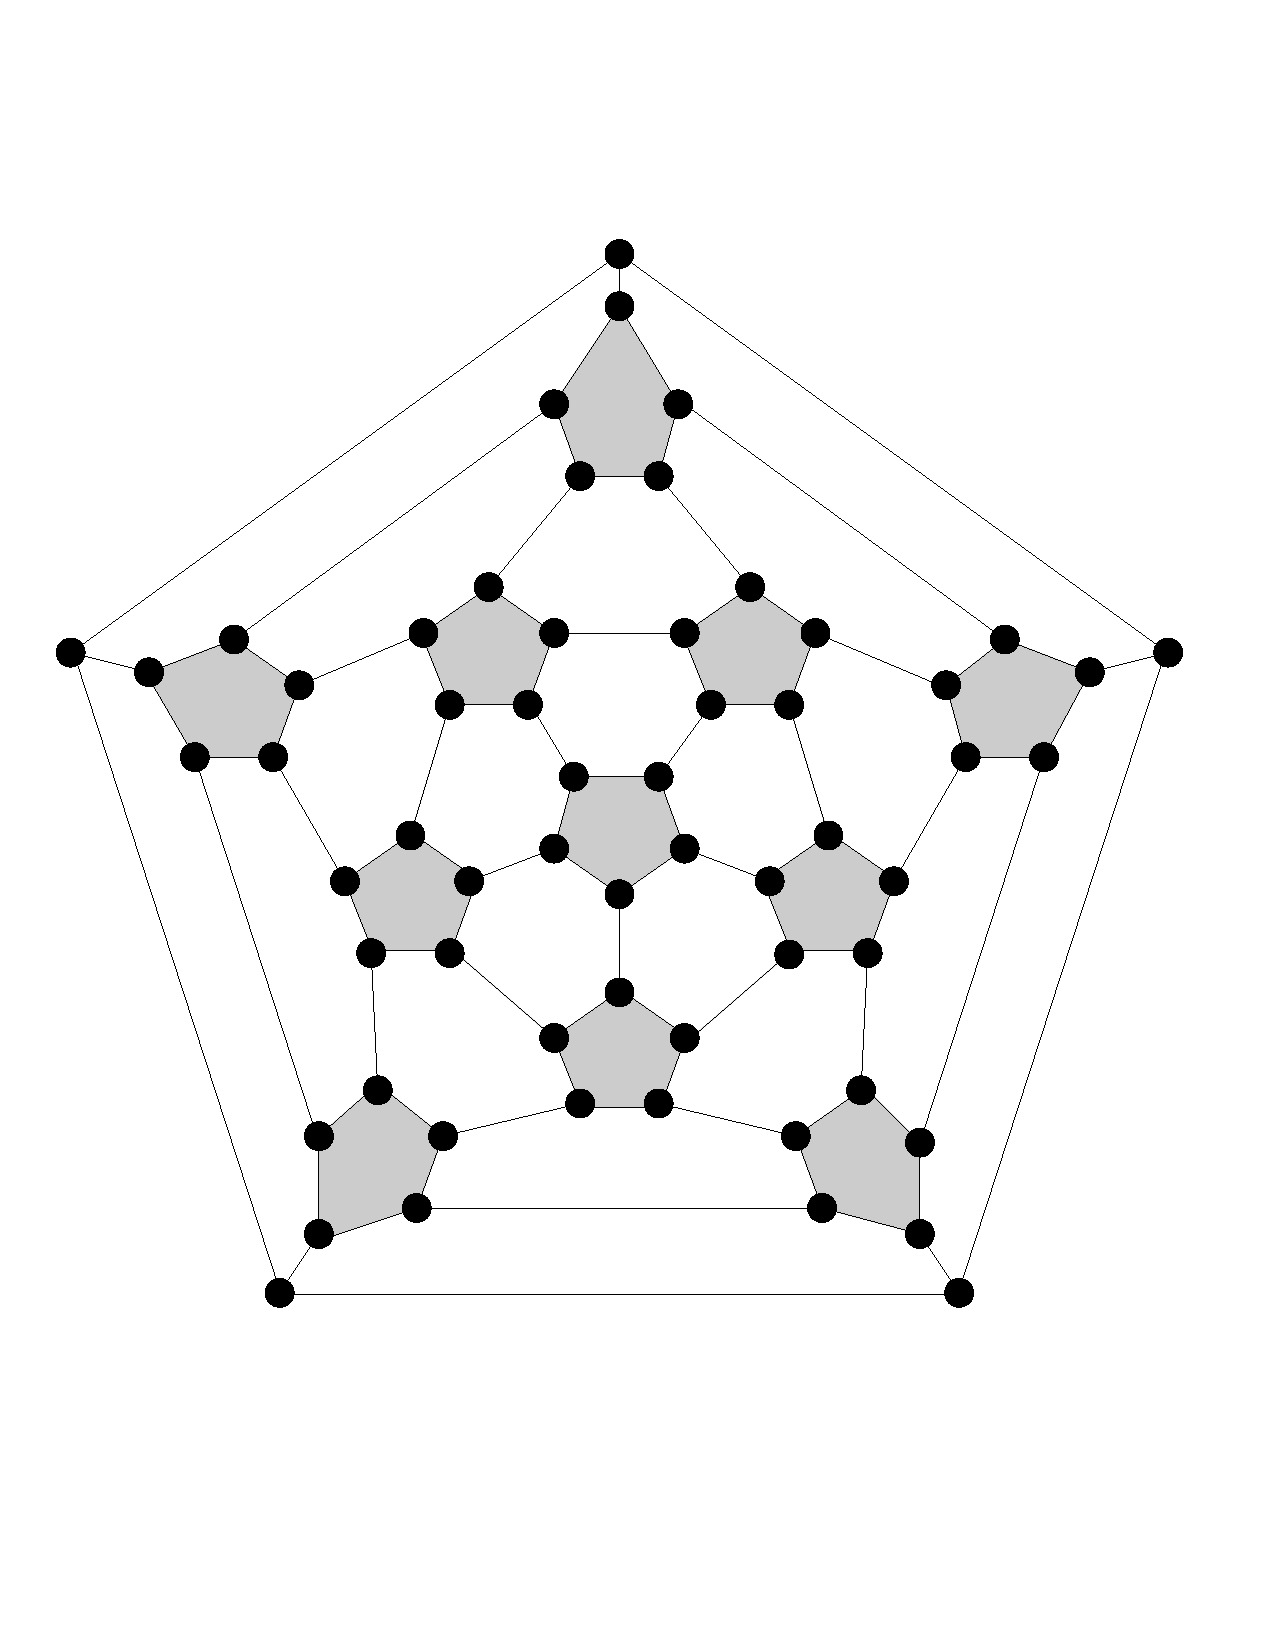
\includegraphics{PicJointSlides/C60.pdf}}
\bigskip
%$C_{60}(I_h)$, $(p,q)$=$(1,1)$\\
%tr, Icosahedron\end{minipage}
\end{minipage}
\begin{minipage}{61mm}
\resizebox{6.1cm}{!}{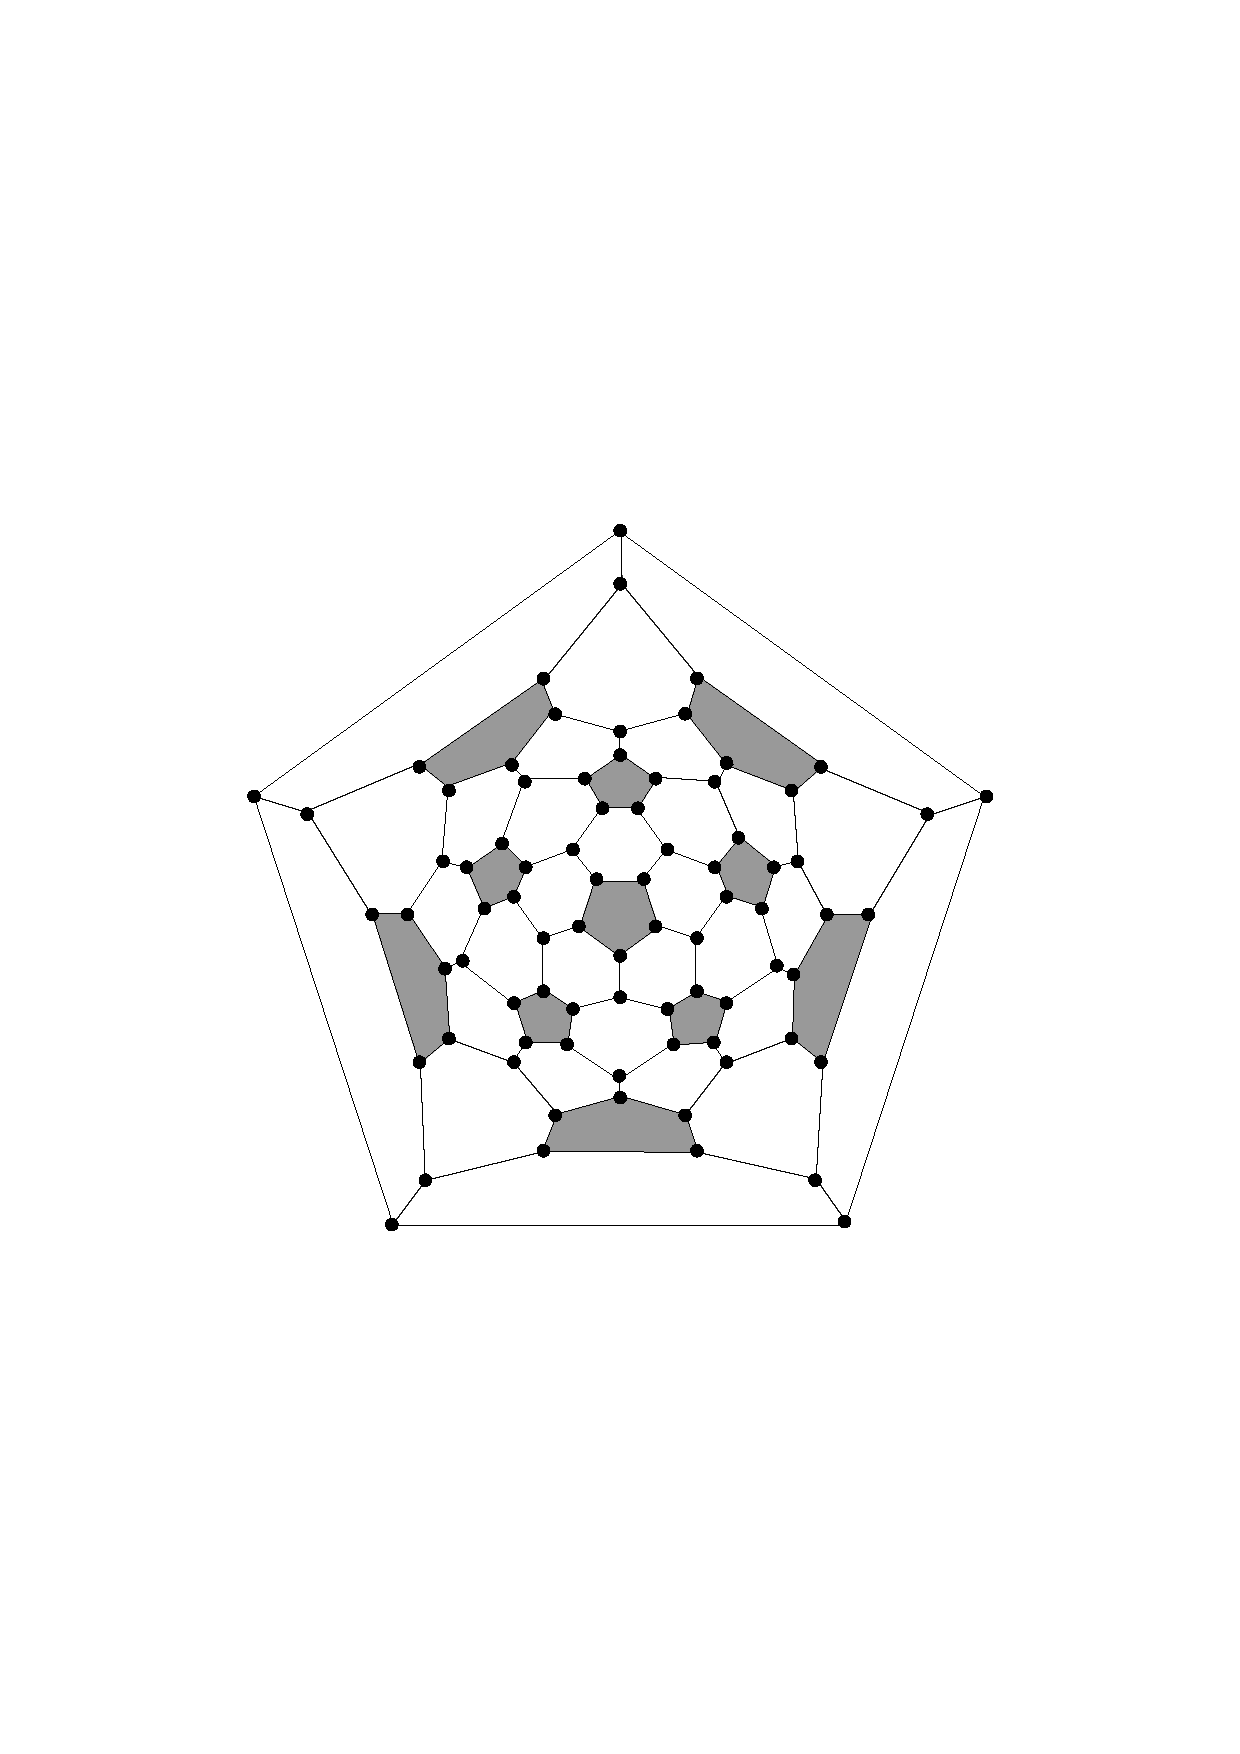
\includegraphics{PicJointSlides/C80.pdf}}
%\vspace{-1cm}
%$C_{80}(I_h)$; $(p,q)$=$(2,0)$\\
% Chamfered $C_{20}(I_h)$


 \end{minipage}\vspace{-13mm}

This construction:
% amounts 
 parameterization by Eisenstein integer $p$+$q\omega$.
\end{center}



\end{frame}





\begin{frame}\frametitle{Extended family 
%Close (i.e., also on $\mathbb{S}^2$) and of interest relatives 
%)Extended family 
of fullerenes; main considered ones are:}
\vspace{-3mm}
%Besides parabolic  
\begin{itemize}
\item 

\textcolor{red}{$(\{a, b\}; k)$} on $\mathbb{S}^2$,  $\mathbb{P}^2$, $\mathbb{T}^2$ or $\mathbb{K}^2$, i.e., $k$-valent maps
with  only $a$- and $b$-gonal faces, of \textcolor{blue}{curvature $1+\frac{i}{k}-\frac{i}{2} 
 %\textcolor{red}{
 \ge 0$} for $i=a,b$.
%($p_c$$=$$1$) and nanocones  $(\{5, 6\}, 3)$-$%\mathbb{E}^2$,

%\begin{itemize}
\item  \textcolor{red}{$b$-icosahedrites}, i.e., $(\{3, b\}, 5)$-$\mathbb{S}^2$ with $b $$\ge $$4$. 
\item  \textcolor{red}{$G$-fulleroids}, i.e., $(\{5, b\}, 3)$-$\mathbb{S}^2$ with $b $$> $$6$ and symmetry $G$.

\item  \textcolor{red}{$c$-disk-fullerenes}, i.e.,   $(\{5, 6, c\}, 3)$-$\mathbb{S}^2$ with $p_c=1$.

\item  \textcolor{red}{$c$-near-fullerenes} $(\{5, 6, c\}, 3)$-$\mathbb{S}^2$, 
%($c$$>$$6$), 
 with all $5$- and $c$-gons forming $\min (12,p_c)$ \textcolor{blue}{lego}  
 (isomorphic  disjoint clusters of faces)
 
 especially,  \textcolor{red}{lego-like fullerenes} $(\{5, 6\}, 3)$-$\mathbb{S}^2$, 
%($c$$>$$6$), 
 with all faces forming $\min (p_5,p_6)= \min (12,p_6)$ %\textcolor{blue}{
 legos. 
 %(isomorphic  disjoint clusters of faces). \pause 

%Haeckel, 1887: $(\{5, 6, 7\}, 3)$- and $(\{5,6, 8\}, 3)$-$\mathbb{S}^2$
%representing skeletons of radiolarian zooplankton {\em Aulonia hexagona}.

%\item  \textcolor{red}{$c$-disk-fullerenes}, i.e.,   $(\{5, 6, c\}, 3)$-$\mathbb{S}^2$ with $p_c=1$.\pause
\item \textcolor{red}{Azulenoids}, i.e., $(\{5,6,7\},3)$-$\mathbb{T}^2$; such tori have $p_5 = p_7$.
\item \textcolor{red}{Schwartzits}, i.e., $(\{ 6, 7\}, 3)$- and 
$(\{ 6, 8\}, 3)$-maps of genus $g \ge 2$
on minimal surfaces of constant negative curvature.
\item \textcolor{red}{Plane fullerenes}, i.e., 
 $(\{5, 6\}, 3)$-$\mathbb{E}^2$; such planes have $p_5\le 6$. 
 
\item Also, \textcolor{red}{space fullerenes} ($\mathbb{E}^3$-tilings by fullerenes) and
%, most general,   
\textcolor{red}{fullerene manifolds} (manifolds whose
$2$-faces are only  $5$- or $6$-gonal).

\end{itemize} 
\end{frame}


\begin{frame}\frametitle{Main considered properties of those maps} 
\vspace{-2mm}
\begin{itemize}

\item Usual ones: 
symmetries, computer enumeration (when feasible), generation, connectivity and so on.
%\vspace{5mm}
\item  Parameterization by complex numbers, esp.   Goldberg--Coxeter construction ($1$-parameter case) using 
%Plane tilings $\{4^4\}$, $\{3^6\}$ and 
 %complex 
 rings 
$\mathbb{Z}[\omega]$ and 
$\mathbb{Z}[i]$.
%\vspace{5mm}

\item
By analogy with $v$-, $p$-vectors enumerating map's vertices and faces, edges are represented by \textcolor{blue}{
$z$-vector} enumerating \textcolor{blue}{zigzags} (left-right circuits  doubly covering  edge-set). Main interesting  cases: \textcolor{red}{knot} (unique zigzag),
 \textcolor{red}{pure} (no zigzag self-intersects) and  \textcolor{red}{tight} (no \textcolor{blue}{railroad}, i.e. pair of "parallel" zigzags) maps. Similar 
 theory is build for \textcolor{blue}{central circuits} of even-valent 
 %Eulerian 
  maps. 
 \end{itemize} 
%\vspace{5mm}
%Besides lego-like and near-parabolic maps,
%relevant papers, 
This material, except lego-like and near-parabolic maps, to appear,
 is presented  in
  our  books:
%which complemented previous book: 
M.Deza and M.Dutour Sikiri\'{c}, {\em Geometry of Chemical Graphs}, Cambridge University Press, 2008, and 
%its follow-up 

M.Deza, M.Dutour Sikiri\'{c} and M.Shtogrin, {\em Geometric Structure of Chemistry-relevant Graphs},
%: zigzags and central circuits Structure Theory}, 
Springer, 2015.
\end{frame}

\section[General]{$8$  families of parabolic $(\{a,b\};k)$-spheres}



%\textcolor{red}{Fullerene manifolds}}
%\\[4mm]{\Huge \textcolor{red}{surfaces}
%}








\frame{
\begin{center}
\begin{tabular*}{7cm}{c}
\\[-0.5cm]\\
{\Huge 
%\textcolor{blue}{I. }
\textcolor{red}{Fullerenes 
and other $7$}}\\
%$8$  families of parabolic}}
[0.5mm]
{\Huge \textcolor{red}{families of parabolic}}\\
%$(\{a,b\};k)$-spheres}}\\
[0.5mm]{\Huge \textcolor{red}{$(\{a,b\};k)$-spheres}}

%[2mm]{fullerenes 
%$(\{5,6\},3)$-$\mathbb{S}^2$}\\ 
%${and $7$ brotherly tribes} 

\end{tabular*}
\end{center}}


%\\[4mm]{\Huge \textcolor{red}{
%with small $p_b$: listings} }
%\end{tabular*}\end{center}}








\begin{frame}\frametitle{$(R,k)$-spheres:  
 \textcolor{red}{curvature} $\kappa_i$=$1$+$\frac{i}{k}-\frac{i}{2}$
%+2k$-$i(k$-$2)$
of  $i$-gons}
\vspace{-2mm}
\begin{itemize}
\item Fix $R\subset \mathbb{N}$. An  \textcolor{red}{$(R,k)$-sphere}  is 
a $k$-regular, $k\ge 3$,  map on 
%the sphere 
$\mathbb{S}^2$ 
whose faces are $i$-gons,
%have {\em gonalities} 
%(numbers of sides) 
$i\in R$. Let $m$=$\min$
%\{i\in R\}$
 and $M$=$\max_{i\in R}i$.
 
%A  \textcolor{red}{$(\{a,b\};k)$-sphere} is an $(R,k)$-sphere 
%with $R=\{a,b\}$.

\item Let $v,e$ and $f=\sum_{i}p_i$ be the map's numbers of 
vertices, edges and faces, where $p_i$ is the number 
of $i$-gonal faces. 
%Clearly,
%$k$-regularity implies 
So, $kv$=$2e$=$\sum_{i}ip_i$ and  
 %\textcolor{blue}
 {\em Euler formula $v-e+f=2$}
%=$\frac{2e}{k}$-$e$+$f$=$\frac{2-k}{k}e$+$\sum_ip_i$
%=
%$\sum_{i}p_i\left(\frac{i(2-k)}{2k}+1\right)$
become   \textcolor{blue}{$2$=$\sum_{i}p_i\kappa_i$}, where 
$\kappa_i$=$1$+$\frac{i}{k}-\frac{i}{2}$ is 
%$C_i$=$\frac{1}{k}$+$\frac{1}{i}-\frac{1}{2}$ is  
the \textcolor{red}{curvature} of $i$-gons.

\item $\kappa_m$$\ge $$0$ implies $m$$<$$\frac{2k}{k-2}$; so, 
 $m$$\ge$$3$, 
%$2k$-$m(k$-$2)>0$ 
 implies $3\le m,k\le 5$,
%So, $m$$<$$\frac{2k}{k-2}$.For $m$$\ge$$3$, 
%$2k$-$m(k$-$2)>0$ it implies $3\le m,k\le 5$,
i.e.  $5$ Platonic 
%pairs of 
parameters
% pairs
%Besides the cases  $k$=$2$ ($m$-cycle) and $m$=$1,2$, it holds
%$\frac{2k}{k-2}>m>2<k<\frac{2a}{a-2}$, i.e.,
$(m,k)$=$(3,3)$, $(4,3)$, $(3,4)$, $(5,3)$, $(3,5)$.
\pause

\item $(R,k)$-sphere is \textcolor{red}{elliptic} if 
%\item If 
\textcolor{blue}{$M$$<$$\frac{2k}{k-2}$}, i.e., $\min_{i\in 
R}\kappa_i>0$;  then 

either  
1) $k=3$, $M\le 5$,  or 2) $k\in \{4,5\}$,  $M\le 3$.
%$(M,k)$=$(\le 5,3),\,(\le 3,4),\,(\le 3,5)$. 

So, for $m\ge 3$, such are only 
Octahedron, 
Icosahedron and 

$10$ $(\{3,4,5\},3)$-spheres: $8$ dual 
 \textcolor{blue}{deltahedra} and the Cube's  truncations on $1$ or $2$ 
opposite vertices (\textcolor{blue}{D\"{u}rer octahedron}).

In other words, five Platonic  and seven $(\{3,4,5\},3)$-spheres.
\end{itemize}

\end{frame}

\begin{frame}\frametitle{Parabolic $(R,k)$-spheres}

\begin{itemize}

\item $(R,k)$-sphere is \textcolor{red}{parabolic} if 
 \textcolor{blue}{$M$=$\frac{2k}{k-2}$}, i.e. $\min_{i\in 
R}\kappa_i$\textcolor{red}{=$0$}.  

So, 
$(M,k)$=$(6,3),\,(4,4),\,(3,6)$ (Euclidean parameter pairs).
% of parameters.  

Exclusion
of
$i$-faces with $\kappa_i$$<$$0$ simplifies enumeration, while
 number $p_M$
of {\em flat} ($\kappa_M$=$0$) $M$-gonal faces not being
restricted, there is an infinity of such $(R,k)$-spheres.
% Clearly, all  possible $(M,k)$ are then $(6,3),\,(4,4),\,(3,6)$.
 
%\item Let us see $C_i$=$2k$-$i(k$-$2)$  as the  \textcolor{red}{curvature} 
%of $i$-gonal faces and 
%Euler formula as equality of the total curvature to $4k$.

\item The number of such $v$-vertex $(R,k)$-spheres with 
$|R|$=$2$ increases polynomially with $v$.
%; their set is countable.

Such spheres admit parametrization and description in terms of 
rings of ({\em Gaussian}
if $k$=$4$ and {\em Eisenstein} if $k$=$3,6$) {\em integers}.

%All eight series of such spheres will be considered in detail.\pause

%\item Remaining $(R,k)$-spheres (with 
\item $(R,k)$-sphere is \textcolor{red}{hyperbolic} if 
\textcolor{blue}{$M$$>$$\frac{2k}{k-2}$}, i.e. $\min_{i\in 
R}\kappa_i$\textcolor{red}{$<0$}; it do not 
admit above, in 
general. We  considered only simplest cases, say: \textcolor{blue}{icosahedrites}, i.e. $(\{3,4\},5)$-spheres,
% (number  of such $v$-vertex  spheres  grows at least exponentially with $v$) 
and  special $(\{a,b,c\};k)$-spheres: those
%with $c\ge 7$
 with $p_b=0$  \textcolor{blue}{or}
 $p_c=0, p_b\le 3$ 
 \textcolor{blue}{or} 
$p_c=1$  \textcolor{blue}{or}  $a$- and $c$-gons forming  disjoint isomorphic clusters).
%)\textcolor{blue}{fulleroids}, i.e. $(\{5,b\},3)$-spheres with $b\ge 7$.

%; their set is a continuum.  
 
\end{itemize}\end{frame}

\begin{frame}\frametitle{ $(R,k)$-maps on general surface $\mathbb{F}^2$
}
\vspace{-1mm}
\begin{itemize}

\item Given $R\subset \mathbb{N}$ and a surface $\mathbb{F}^2$, an
\textcolor{red}{$(R,k)$-$\mathbb{F}^2$} is
a $k$-regular map  on surface $\mathbb{F}^2$
whose faces have gonalities $i\in R$.

\item
The \textcolor{red}{Euler characteristic $\chi ({\mathbb{F}^2})$} is $v$-$e$+$f$=
%$, where $v,e$ and $f=\sum_{i}p_i$ are the numbers of its vertices, edges and faces.
%\item Since   $kv$=$2e$=$\sum_{i}ip_i$,   Euler formula \textcolor{blue}{$\chi=v-e+f$}
 % becomes Gauss-Bonnet-like one
$\textcolor{blue}{\sum_{i}p_i\kappa_i}$, 
where $\kappa_i$=$1$+$\frac{i}{k}-\frac{i}{2}$ and $p_i$ is the number of $i$-gons. So, elliptic and, with $|R|$$>$$1$,
 parabolic $(R,k)$-maps exist only on $\mathbb{S}^2$ and $\mathbb{P}^2$.
%\pause

\item In fact, all connected {\em closed} (compact and without boundary) irreducible 
surfaces $\mathbb{F}^2$ with \textcolor{blue}{$\chi ({\mathbb{F}^2})$$\ge$$ 0$}
are (with $\chi=2,0,1,0$, 
respectively):
\textcolor{blue}{orientable}: sphere $\mathbb{S}^2$, torus $\mathbb{T}^2$ 
 and 
 
 \textcolor{blue}{non-orientable}:
real projective 
%(elliptic) 
 plane
 $\mathbb{P}^2$ and Klein bottle $\mathbb{K}^2$.
\pause

\item
Again, let our $(R,k)$-maps be
\textcolor{red}{parabolic}, i.e.,
$\min_{i\in R}\kappa_i=0$.

Then  \textcolor{blue}{$M$=:$\max\{i\in R\}$=$\frac{2k}{k-2}$}, 
and $(M,k)$=\textcolor{blue}{$(6,3),\,(4,4),\,(3,6)$}.


\item Also, there are infinity of parabolic maps $(R,k)$-$\mathbb{F}^2$, since the number
$p_M$ of {\em flat} ($\kappa_M$=$0$) faces is not restricted.

\item  %So, \textcolor{blue}{$\chi ({\mathbb{F}^2})$$\ge$$ 0$} with $\chi ({\mathbb{F}^2})$=$0$ iff 
Also, if $\chi ({\mathbb{F}^2})$=${\sum_{i}p_i\kappa_i}$=
$0$, i.e.  ${\mathbb{F}^2}$ is $\mathbb{T}^2$ or $\mathbb{K}^2$, then $R$=$\{M\}$ 
\end{itemize}\end{frame}

\begin{frame}\frametitle{$8$ families of parabolic $(\{a,b\};k)$-\textcolor{red}{spheres}}



\begin{itemize}

\item An \textcolor{red}{$(\{a,b\};k)$-sphere} is an  $(R,k)$-sphere
with $R=\{a,b\}$, $1\le a < b$. $\,$ 
It has  \textcolor{blue}{$v$$=$$\frac{1}{k}(ap_a+bp_b)$} vertices.
\item 
%Parabolicity implies 
Such parabolic sphere has $b=\frac{2k}{k-2}$;$\,$
%, $r=\frac{2k}{k-2}$
 so, $(b,k)$=
\textcolor{blue}{$(6,3),\,(4,4),\,(3,6)$} 
and
Euler formula become

$2=\kappa_ap_a$=$(1+\frac{a}{k}-\frac{a}{2})p_a$=$(1-\frac{a}{b})p_a$.


\item So, \textcolor{blue}{$p_a=\frac{2b}{b-a}$}
%, $v=\frac{1}{k}(ap_a+bp_b)$ 
and all possible
$(a,p_a)$ are:

 $(5,12),\, (4,6),\, (3,4),\, (2,3)$ for 
$(b,k)$=\textcolor{blue}{$(6,3)$};
         
$(3,8),\, (2,4)$ for $(b,k)$=\textcolor{blue}{$(4,4)$}; $\,\,$

$(2,6),\, (1,3)$ for $(b,k)$=\textcolor{blue}{$(3,6)$}.

\item Those $8$ families can be seen  as spheric analogs of the 
regular plane partitions $\{6^3\},\,\{4^4\},\,\{3^6\}$ with $p_a$ 
{\em disclinations} ("defects") $\kappa_a$   added to get the 
curvature $2$
of the sphere.
% $\mathbb{S}^2$.


 \end{itemize}\end{frame}

\begin{frame}\frametitle{$8$ parabolic families: existence criterions}
\vspace{-3mm}
\textcolor{blue}{Gr\H{u}nbaum--Motzkin, 1963}: criterion for $k$=$3\le a$;

\textcolor{blue}{Gr\H{u}nbaum, 1967}:
 for $(\{3,4\},4)$-spheres;

\textcolor{blue}{Gr\H{u}nbaum--Zaks, 1974}: for $a=1,2$.

\hspace{-2cm}{\scriptsize
\begin{center}
\begin{tabular}{||c|c||c|c|c|c||c|c||}
\hline
\hline
$k$ & $(a,b)$ & smallest one & it exists if and only if & $p_a$ & $v$&Ord&Gr\\
\hline\hline
$3$ & $(5,6)$ & Dodecahedron & $p_{6} \neq 1$ & $12$
&$20$$+$$2p_6$&$v^9$&28\\  \hline
$3$ & $(4,6)$ & Cube & $p_{6} \neq 1$ & $6$ &$8$$+$$2p_6$&$v^3$&16\\ \hline
$4$ & $(3,4)$ & Octahedron & $p_{4} \neq 1$ &
$8$ &$6$$+$$p_4$&$v^5$&18\\ \hline
$6$ & $(2,3)$ &Bundle$_6$=$6$$\times$$ K_2$ & $p_3$ is even&
$6$ &$2$$+$$\frac{p_3}{2}$&$v^4$&22\\ \hline \hline
$3$ & $(3,6)$ &Tetrahedron  & $p_6$ is even&
$4$ &$4$$+$$2p_6$&$v$&5\\ \hline
%$3$ & $(2,6)$ &$3\times K_2$  & $p_6$=$(k^2+kl+l^2)-1$&
%$3$ &$2+2p_6$\\ \hline \hline
%$4$ & $(3,4)$ & Octahedron & $p_{4} \neq 1$ &
%$8$ &$6+p_4$\\ \hlinehline
$4$ & $(2,4)$ &Bundle$_4$=
 $4$$\times$$ K_2$ & $p_4$ is even&
$4$ &$2$$+$$p_4$&$v$&5\\ \hline \hline
%$6$ & $(2,3)$ & $6\times K_2$ & $p_3$ is even&
%$6$ &$2+\frac{p_3}{2}$\\ \hline
$3$ & $(2,6)$ &Bundle$_3$=$3$$\times$$ K_2$  & $p_6$=$(k^2$$+$$kl+$$l^2)$$-$$1$&
$3$ &$2$$+$$2p_6$&$v$&2\\ \hline
$6$ & $(1,3)$ &Trifolium  & $p_3$=$2(k^2$$+$$kl+$$l^2)$$-$$1$&
$3$ &$\frac{1+p_3}{2}$&$v$&3\\ \hline\hline\hline\hline
$5$ & $(3,4)$ &Icosahedron  & $p_4\neq 1$&
$2p_4$+$20$ &$2p_4$+$12$&exp&38\\ \hline\hline
\end{tabular}
\end{center}
}
%\pause

%$(\{3,6\},3)$- (\textcolor{blue}{Gr\H{u}nbaum-Motzkin, 1963}) and
%$(\{2,4\},4)$-spheres (\textcolor{blue}{Deza-Shtogrin, 2003})
%admit a simple $2$-parametric description.
\end{frame}


\begin{frame}\frametitle{$8$ families of parabolic $(\{a,b\};k)$-spheres}
%\vspace{-3mm}
 \begin{itemize}

\item Let us denote $(\{a,b\};k)$-sphere with $v$ vertices by
\textcolor{red}{$\{a,b\}_v$}.
\bigskip
%\item Euler formula $2=v-e+f=v-\frac{vk}{2}+(p_a+p_b)$ 

%implies also  $v=\frac{a(b-2)}{b-a}+\frac{b-2}{2}p_b=\frac{4a}{2k-a(k-2)}+\frac{2}{k-2}p_b$.

%The members $\{5,6\}_v$ of the family of 
\item $(\{5,6\},3)$- and $(\{4,6\},3)$-spheres are  models of molecules of 
(chemical) \textcolor{blue}{fullerenes} and \textcolor{blue}{boron nitrides}., respectively.
%important in Chemistry.
%of great practical interest.
%$\{5,6\}_{60}(I_h)$: a new  {\em carbon allotrope} $C_{60}$.
%$\{5,6\}_{620}(I)$=$GC_{5,1}(\{5,6\}_{20})$ $\approx$ {\em Callaway 
%golf ball} $\{5,6\}_{660}$.

\item $(\{a,b\},4)$-spheres are minimal projections of  
\textcolor{blue}{alternating links}, 
whose
components are their  {\em central circuits} 
 (those going only ahead) and crossings are the vertices.
%\pause
\bigskip
%\item Let us denote $(\{a,b\};k)$-sphere with $v$ vertices by
%\textcolor{red}{$\{a,b\}_v$}.

%\item By smallest member, Dodecahedron $\{5,6\}_{20}$, Cube 
%$\{4,6\}_8$, 
%Tetrahedron $\{3,6\}_4$,   Octahedron 
%$\{3,4\}_6$ and   $3$$\times $$K_2$ $\{2,6\}_2$, $4$$\times$$K_2$ 
%$\{2,4\}_2$, 
%$6$$\times $$K_2$ $\{2,3\}_2$,
\item \textcolor{red}{Bundle$_m$} is $m\times K_2$. 
\textcolor{red}{Trifolium}  $\{1,3\}_1$ is the {\em $3$-rose} $3\times (aa)$. 
\bigskip


\item \textcolor{red}{$b$-icosahedrites} ($(\{3,b\},5)$-spheres) \textcolor{blue}
%, starting from Icosahedron, 
{are hypebolic} if $b$$>$$3$, $p_b$$>$$0$, since $p_3$=$p_b(3b$-$10)$+$20$ and 
%$b$-gons are hyperbolic. 
$\kappa_b=\frac{10-3b}{10b}<0$.
\end{itemize}
\end{frame}





\begin{frame}\frametitle{Generation of $4$ simplest parabolic $(\{a,b\};k)$-spheres}
\vspace{-2mm}
\begin{itemize}
\item
$(\{3,6\},3)$- (\textcolor{blue}{Gr\H{u}nbaum--Motzkin, 1963}) and
$(\{2,4\},4)$-spheres (\textcolor{blue}{Deza--Shtogrin, 2003})
admit a 
%simple 
 $2$-parametric
 description (by $2$ complex numbers) and also a description by $3$ integers.
\bigskip


\item $1$-parametric description: $(\{2,6\},3)$-spheres are given by the {\em Goldberg--Coxeter
construction}
from  \textcolor{red}{Bundle$_3$} $\{2,6\}_{2}$=$3$$\times$$ K_2$.
\item
$(\{1,3\},6)$-spheres come by this
% {\em Goldberg--Coxeter
construction (extended  on $6$-regular spheres)
from
 \textcolor{red}{Trifolium} $\{1,3\}_{1}$=$3$$\times $$(aa)$.


\bigskip



\item $(\{2,3\},6)$-spheres, except of $6\times K_2$ and $3\times K_3$, are
the duals of  $(\{3,4,5,6\},3)$-spheres with six new
vertices put on  edges.
Example: $(\{5, 6\},3)$-spheres
with $5$-gons organized in 
%six $
$6$ pairs.

\item 
$(\{1,2,3\},6)$-spheres with $v$$>$$3$, except of $5$ infinite series, are
 the duals of  $(\{3,4,5,6\},3)$-$\mathbb{S}^2$ 
 with  splitting (into a $2$-gon or into a $2$-gon, enclosing a $1$-gon) of some edges. 
%With the exception of the following graphs T1, T2 and the spheres of the infinite series depicted in Figures 1, 2, 3 and 4, any ({1, 2, 3}, 6)-sphere with at least one 1-gon is obtained from a ({3, 4, 5, 6}, 3)-sphere by taking the dual and then splitting some edges 
%according to following two schemes:



 \end{itemize}



\end{frame}

%\frame{
%\begin{center}
%\begin{tabular*}{7cm}{c}
%\\[-0.5cm]
%{\Huge 
%%\textcolor{blue}{IV. }
%\textcolor{red}{
%$8$ parabolic families:}}
%%$8$ families:}}
%\\[4mm]{\Huge \textcolor{red}{
%$4$ smallest members}
%}
%\end{tabular*}
%\end{center}
%}



\begin{frame}\frametitle{First four $(\{4,6\},3)$- and
$(\{5,6\},3)$-spheres (fullerenes)}
\vspace{-1.5mm}

\begin{center}
\begin{minipage}[b]{24mm}
\centering
%\resizebox{20mm}{!}{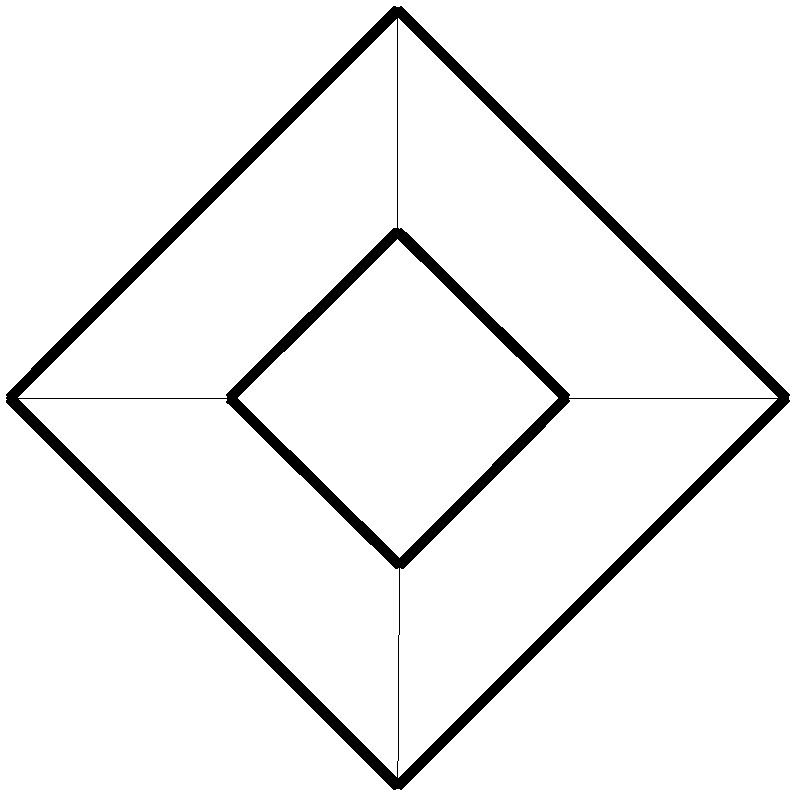
\includegraphics{PicJointSlides/Prism4.pdf}}\par
\resizebox{20mm}{!}{\rotatebox{90}{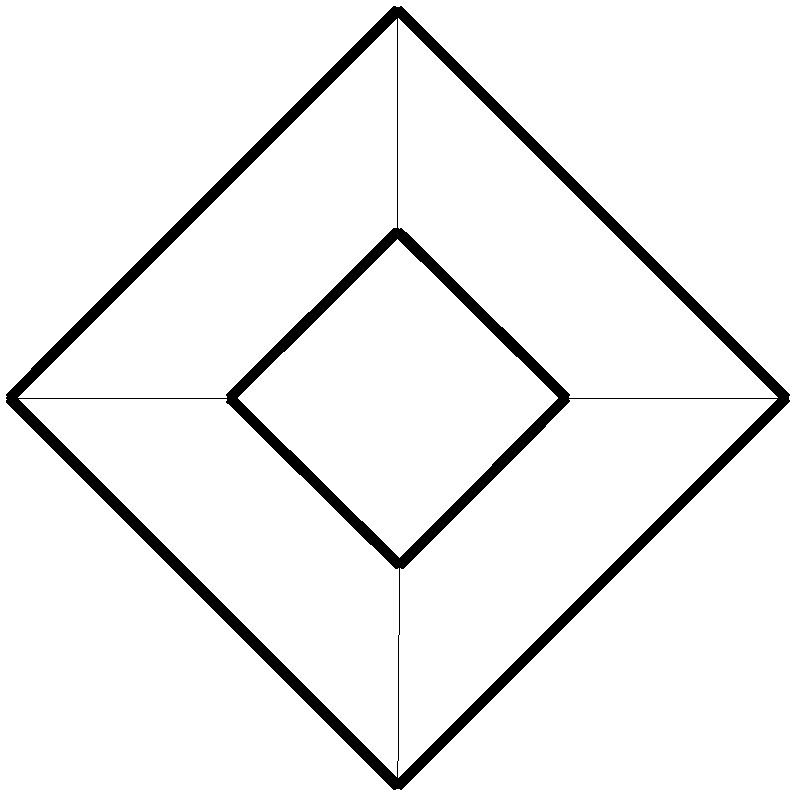
\includegraphics{PicJointSlides/Prism4.pdf}}}\par
$O_h$ ($6^4$)
\end{minipage}
\begin{minipage}[b]{25mm}
\centering
\resizebox{21mm}{!}{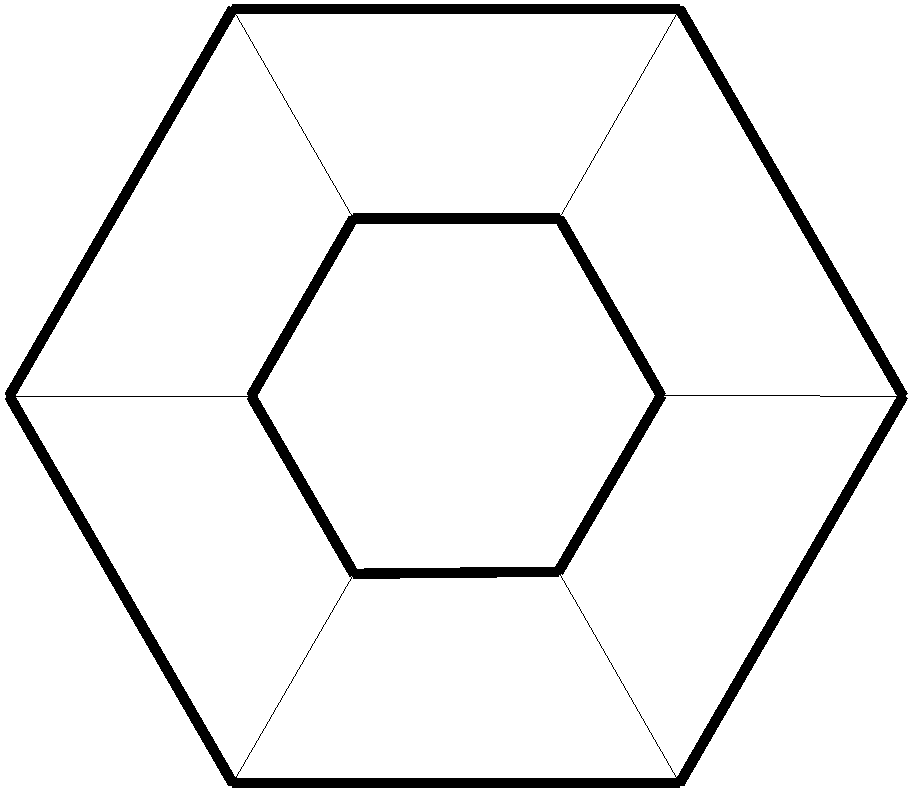
\includegraphics{PicJointSlides/Prism6.pdf}}\par
$D_{6h}$ ($18^2$)
\end{minipage}
\begin{minipage}[b]{24mm}
\centering
%\resizebox{20mm}{!}{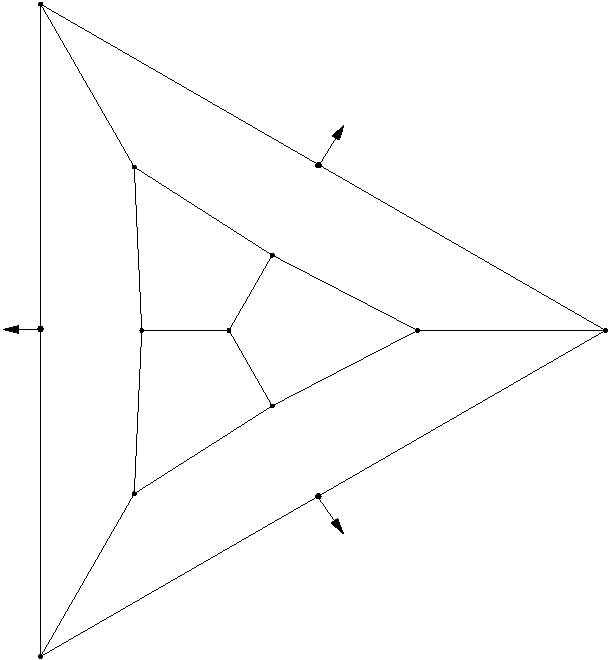
\includegraphics{PicJointSlides/First4nD3hthi.pdf}}\par
\resizebox{20mm}{!}{\rotatebox{90}{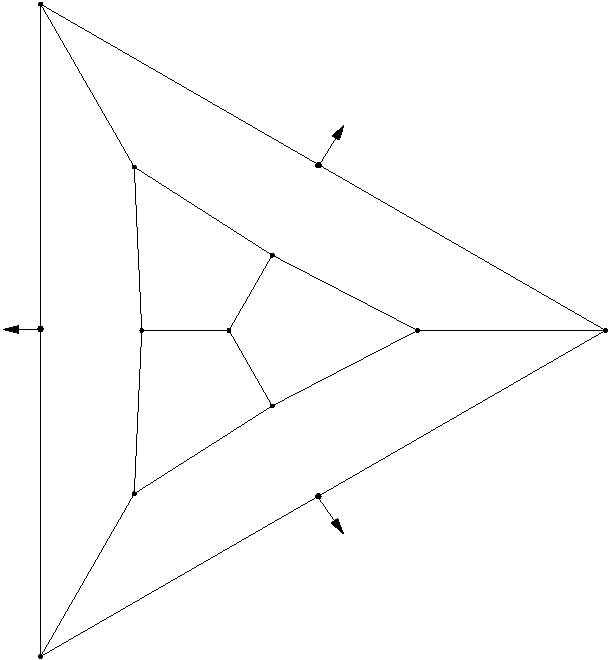
\includegraphics{PicJointSlides/First4nD3hthi.pdf}}}\par
$D_{3h}$ ($6^2;30$)
\end{minipage}
\begin{minipage}[b]{23mm}
\centering
\resizebox{19mm}{!}{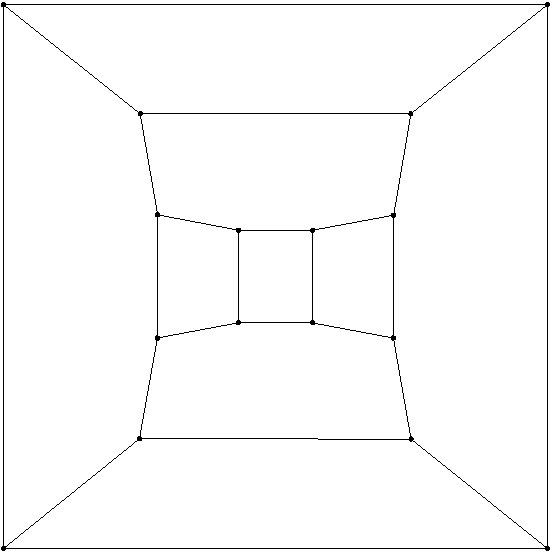
\includegraphics{PicJointSlides/First4nD2dthi.pdf}}\par
$D_{2d}$ ($24^2$)
\end{minipage}
\end{center}


\begin{center}
\begin{minipage}[b]{24mm}
\centering
\resizebox{20mm}{!}{\rotatebox{90}{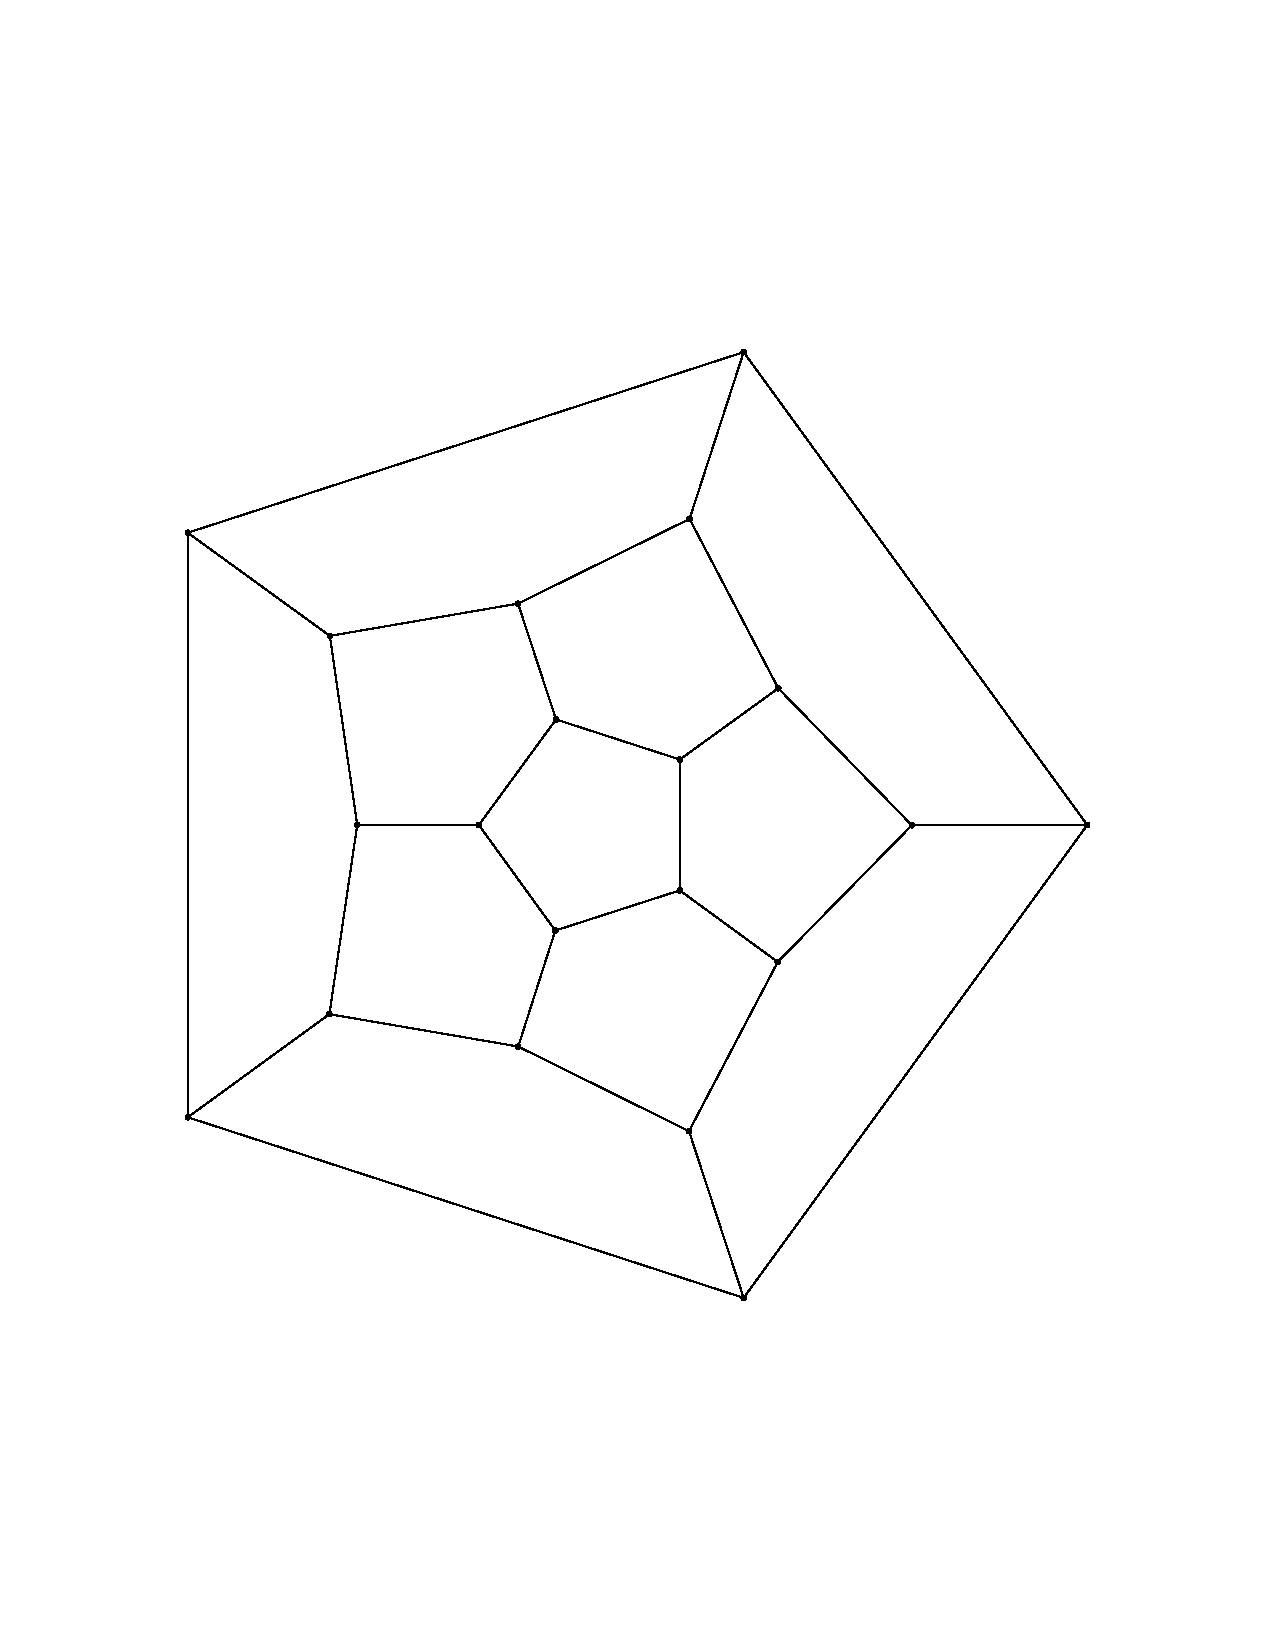
\includegraphics{PicJointSlides/F1.pdf}}}\par
%\resizebox{20mm}{!}{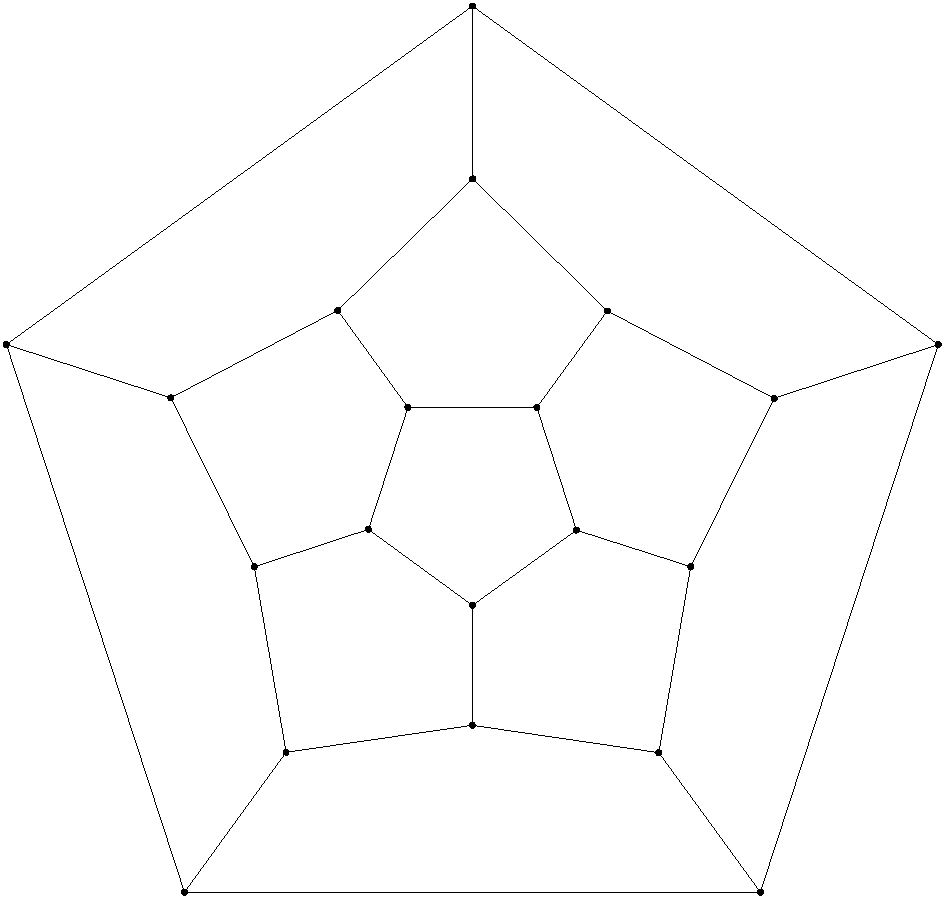
\includegraphics[bb=1 1 440 381,
%clip]{PicJointSlides/Dodecahedron.pdf}}\par
 $I_h$ ($10^6$)
\end{minipage}
\begin{minipage}[b]{24mm}
\centering
\resizebox{20mm}{!}{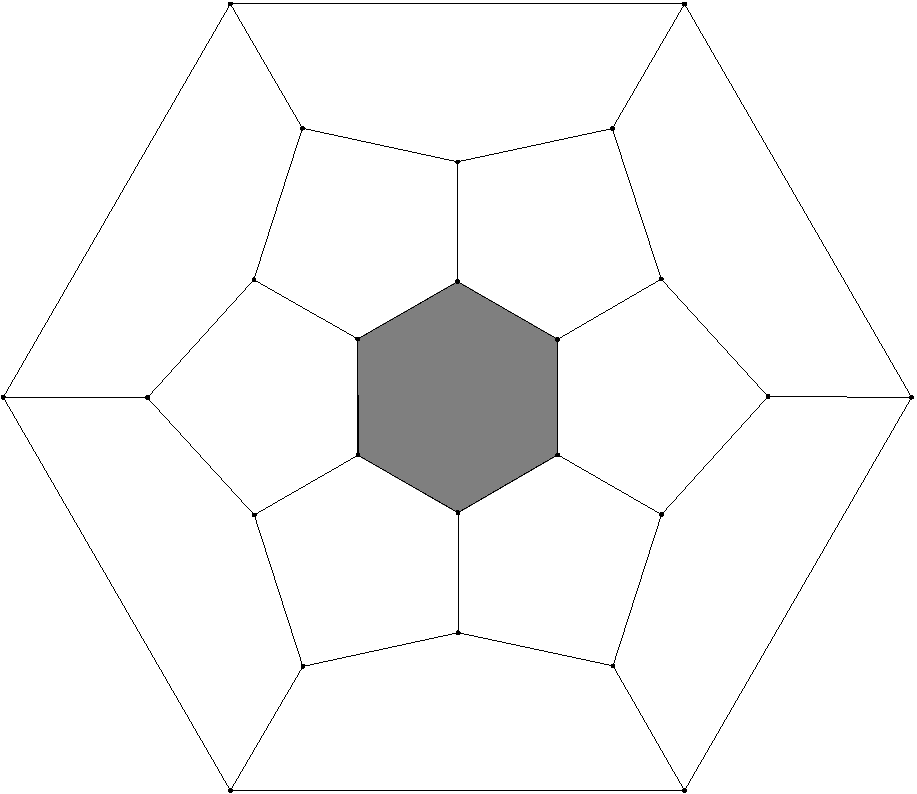
\includegraphics[bb=1 1 440 381,
clip]{PicJointSlides/F2sec.pdf}}\par
 $D_{6d}$ ($12;60$)
%($12;60_{12,12}$)
\end{minipage}
\begin{minipage}[b]{24mm}
\centering
\resizebox{20mm}{!}{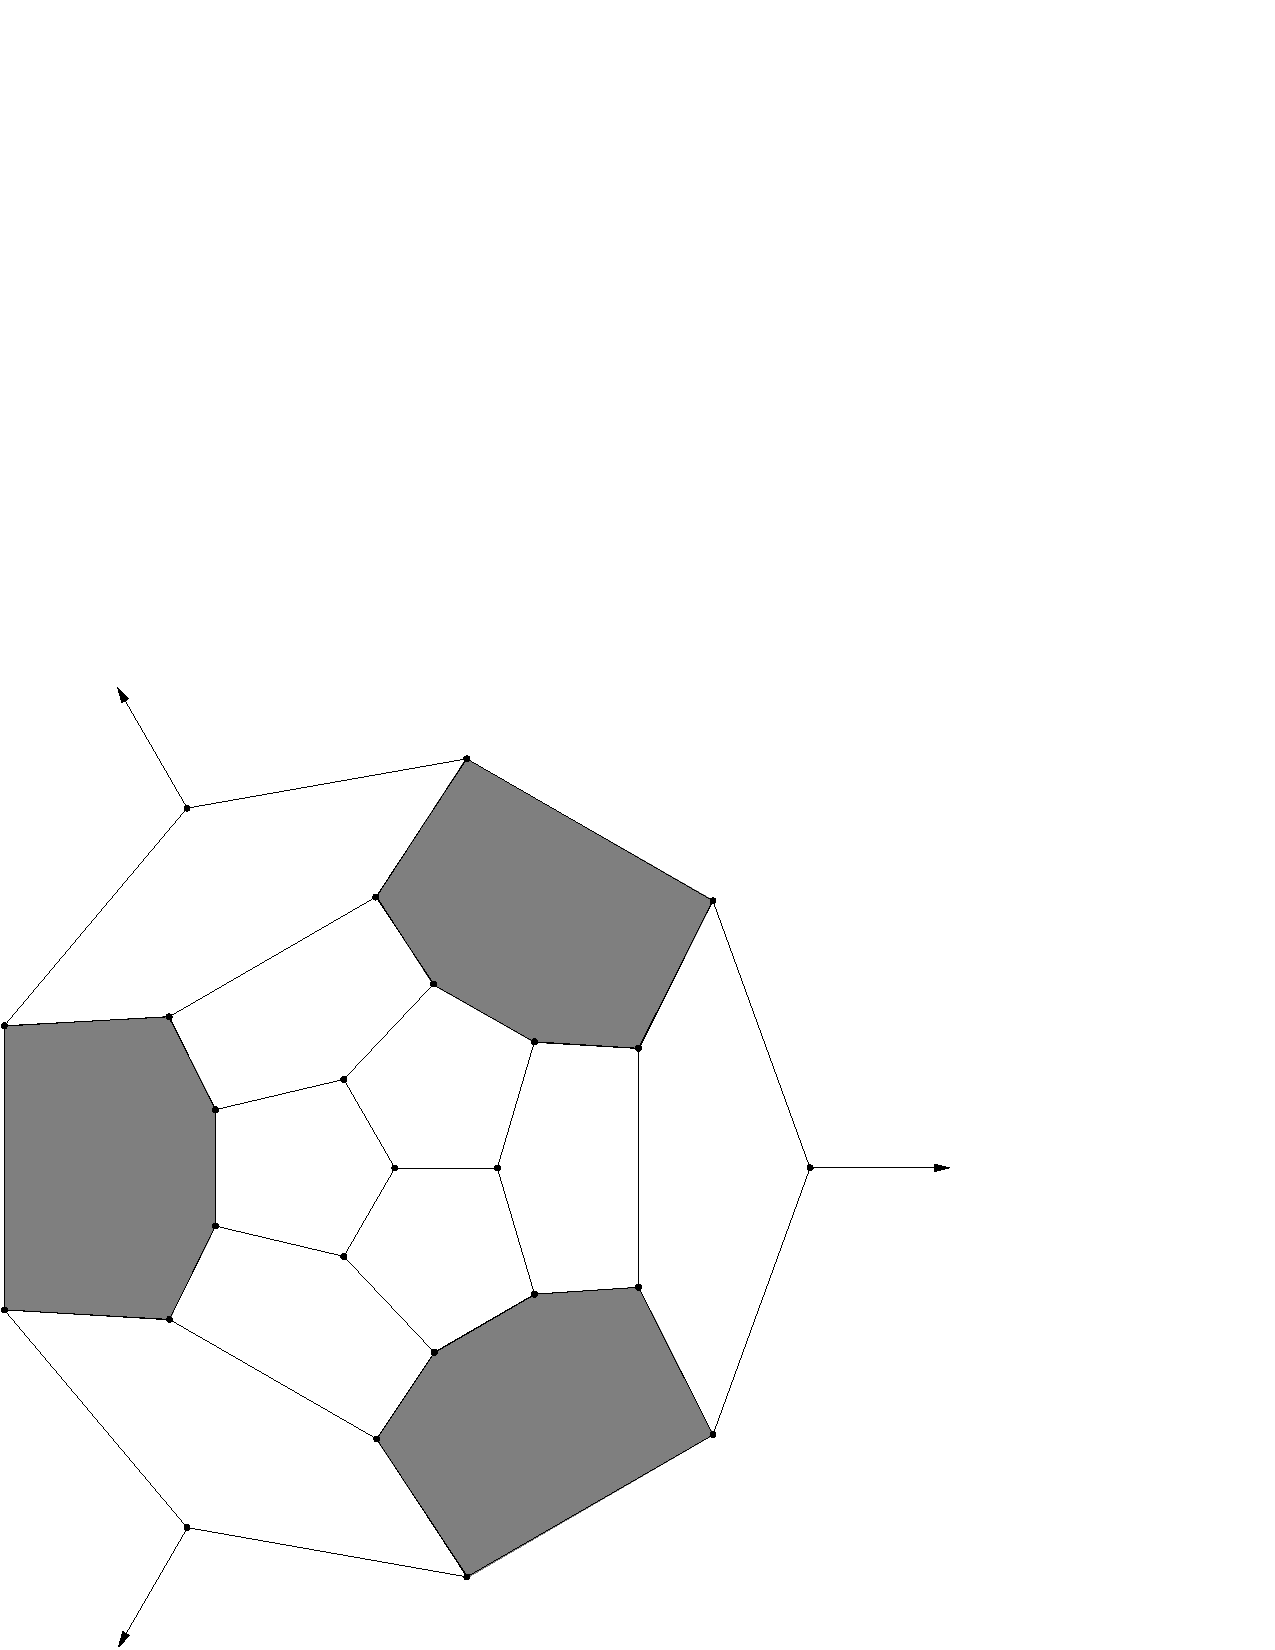
\includegraphics[bb=1 1 457 464,
clip]{PicJointSlides/Picture2.pdf}}\par
 $D_{3h}$ ($12^3;42$)
%($12^3;42_{0,9}$)
\end{minipage}
\begin{minipage}[b]{24mm}
\centering
\resizebox{20mm}{!}{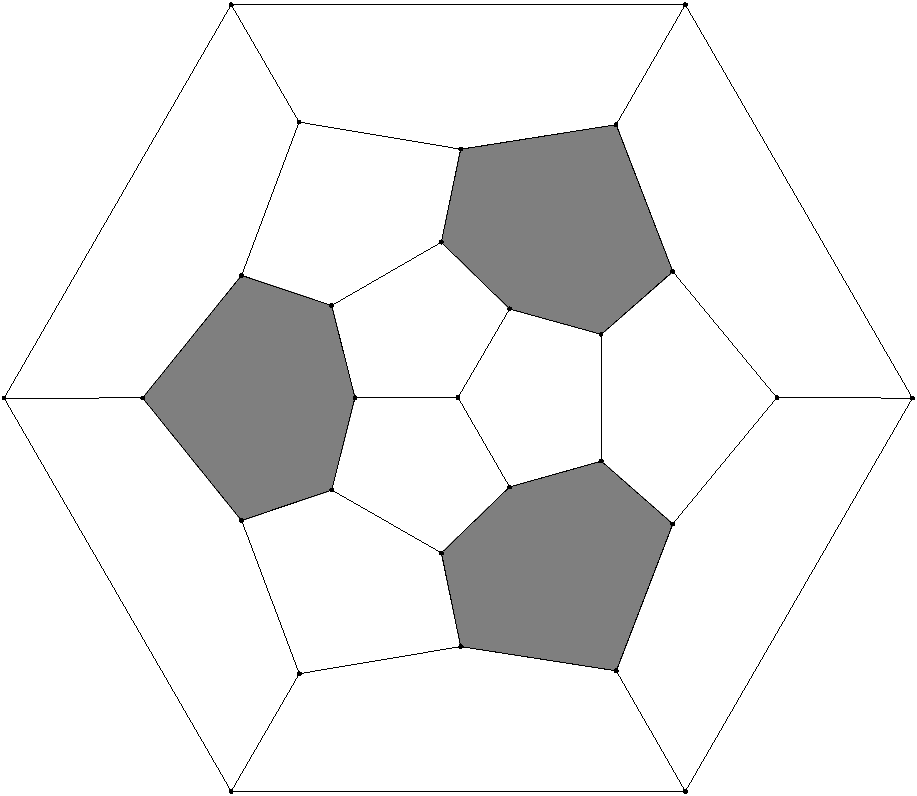
\includegraphics[bb=1 1 439 380,
clip]{PicJointSlides/F4sec.pdf}}\par
 $T_{d}$ ($12^7$)
\end{minipage}\end{center}
\end{frame}

\begin{frame}\frametitle{First four $(\{2,6\},3)$- and
$(\{3,6\},3)$-spheres}
\vspace{-1.5mm}
 Number  of $(\{2,6\}_v$'s is nr. of representations $v$=$2(k^2+kl+l^2)$,
$0\le l\le k$ ($GC_{k,l}(\{2,6\}_2)$). It become $2$ for
$v$=$7^2$=$5^2$+$15$+$3^2$.

\begin{center}
\begin{minipage}[b]{25mm}
\centering
\resizebox{21mm}{!}{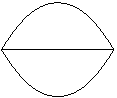
\includegraphics{PicJointSlides/First2nD3h.pdf}}\par
$D_{3h}$ ($6$)
\end{minipage}
\begin{minipage}[b]{23mm}
\centering
\resizebox{19mm}{!}{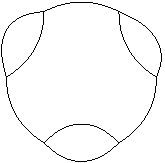
\includegraphics{PicJointSlides/GC11Bundle.pdf}}\par
$D_{3h}$ ($6^3$)
\end{minipage}
\begin{minipage}[b]{18mm}
\centering
\resizebox{16mm}{!}{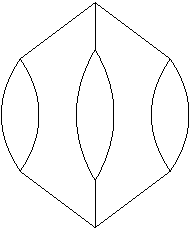
\includegraphics{PicJointSlides/GC20Bundle.pdf}}\par
$D_{3h}$  ($12^2$)
\end{minipage}
\begin{minipage}[b]{28mm}
\centering
\resizebox{22mm}{!}{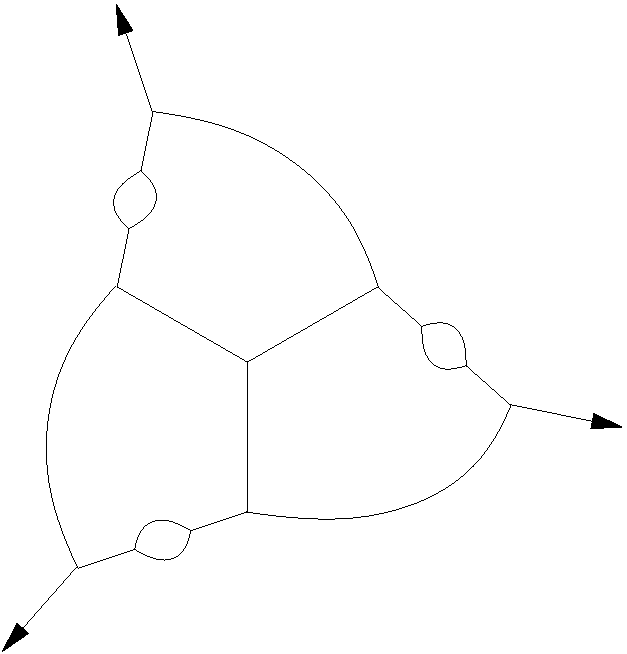
\includegraphics{PicJointSlides/FirstClass2nD3.pdf}}\par
%\resizebox{20mm}{!}{\rotatebox{90}{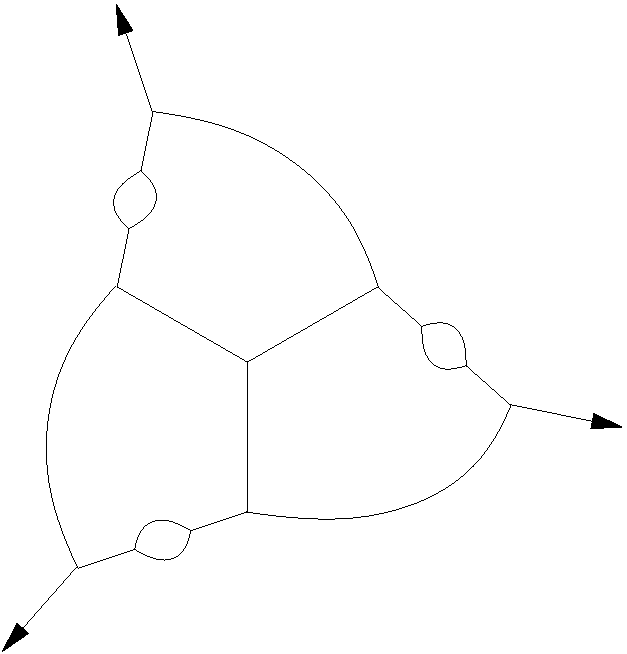
\includegraphics{PicJointSlides/FirstClass2nD3.pdf}}}\par 
$D_{3}$ ($42$)
\end{minipage}
\end{center}

\begin{center}
\begin{minipage}[b]{20mm}
\centering
\resizebox{20mm}{!}{\rotatebox{90}{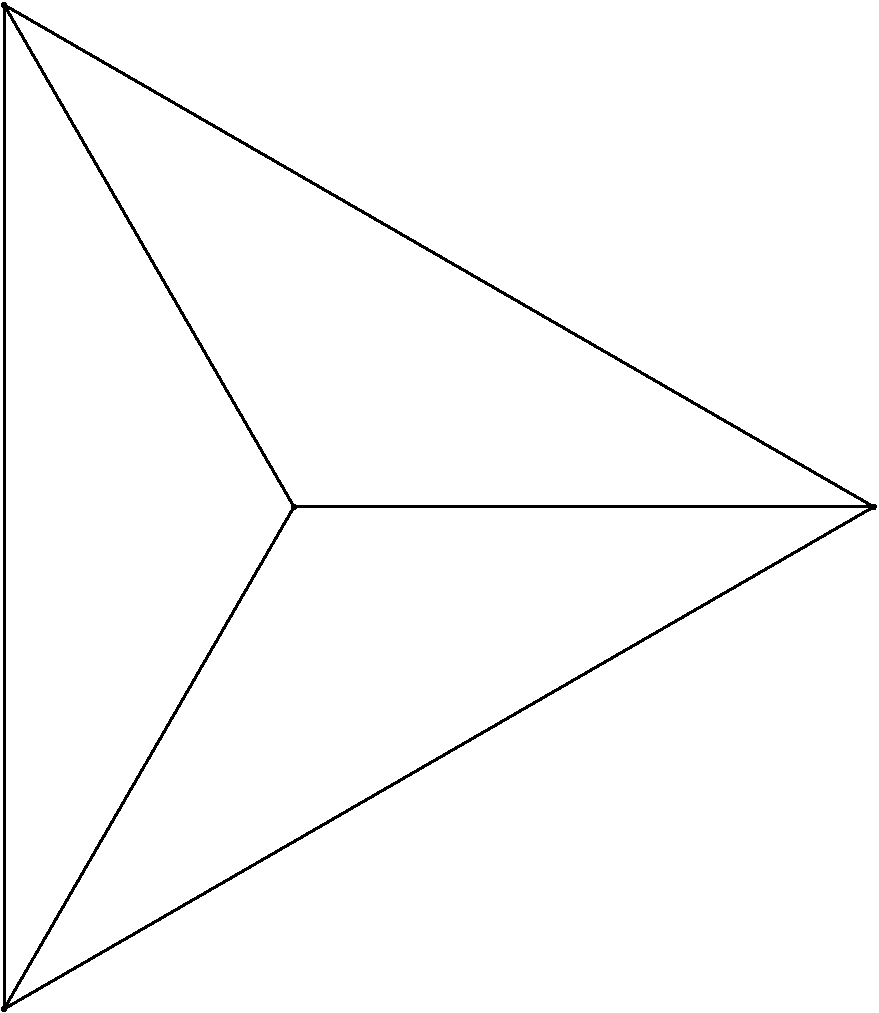
\includegraphics{PicJointSlides/TetrahedronH.pdf}}}\par
$T_d$ ($4^3$)
\end{minipage}
\begin{minipage}[b]{29mm}
\centering
\resizebox{24mm}{!}{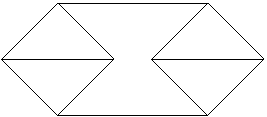
\includegraphics{PicJointSlides/SeqG1.pdf}}\par
$D_{2h}$ ($8^2,4^2$)
\end{minipage}
\begin{minipage}[b]{20mm}
\centering
\resizebox{20mm}{!}{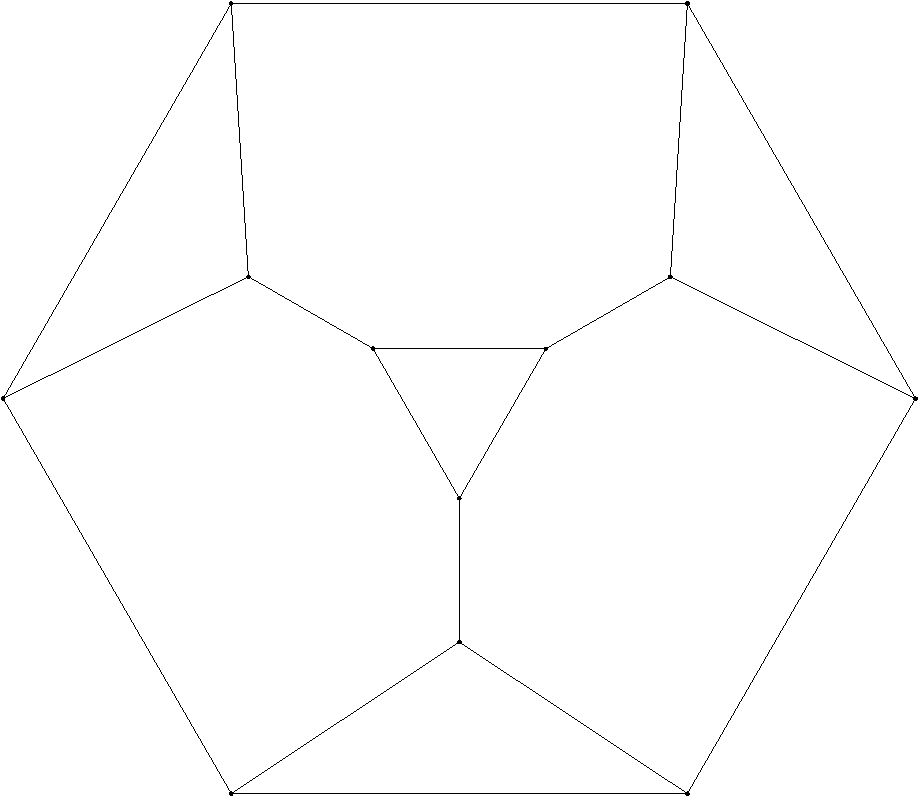
\includegraphics{PicJointSlides/TruncatedTetrahedronNaked.pdf}}\par
$T_d$ ($12^3$)
\end{minipage}
\begin{minipage}[b]{24mm}
\centering
\resizebox{20mm}{!}{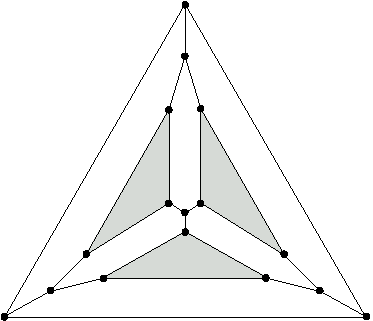
\includegraphics{PicJointSlides/ebe1.pdf}}\par
 $T_d$ $(8^6)$
\end{minipage}
\end{center}
\end{frame}

\begin{frame}\frametitle{First four $(\{2,4\},4)$- and  $(\{3,4\},4)$-spheres}
\vspace{-4mm}
\begin{center}
\begin{minipage}[b]{24mm}
\centering
\resizebox{20mm}{!}{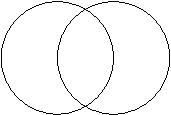
\includegraphics{PicJointSlides/4-hedrite2_1.pdf}}\par
$D_{4h}$ \textcolor{blue}{$2^2_1$} $(2^2)$
\end{minipage}
\begin{minipage}[b]{21mm}
\centering
\resizebox{18mm}{!}{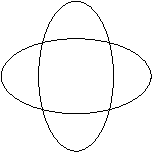
\includegraphics{PicJointSlides/4-hedrite4_1.pdf}}\par
$D_{4h}$ \textcolor{blue}{$4^2_1$}  $(4^2)$
\end{minipage}
\begin{minipage}[b]{29mm}
\centering
\resizebox{24mm}{!}{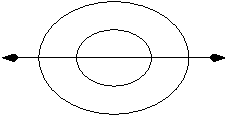
\includegraphics{PicJointSlides/4-hedrite4-2.pdf}}\par
$D_{2h}$ 
\textcolor{blue}{$2$$\times$$ 2^2_1$} 
 $(2^2,4)$ 
\end{minipage}
\begin{minipage}[b]{24mm}
\centering
\resizebox{20mm}{!}{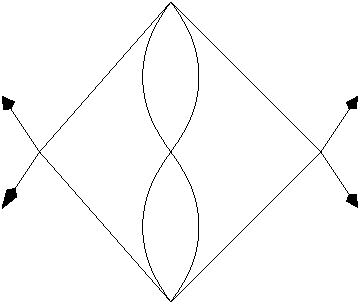
\includegraphics{PicJointSlides/4-hedrite6_1sec.pdf}}\par
%\textcolor{blue}{$6^2_2$}  
$D_{2d}$ \textcolor{blue}{$6^2_2$}  $(6^2)$
\end{minipage}
\end{center}

\begin{center}
\begin{minipage}[b]{24mm}
\centering     
\resizebox{20mm}{!}{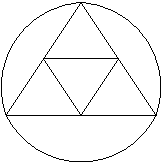
\includegraphics{PicJointSlides/8-hedrite6-1.pdf}}\par
$O_h$ \textcolor{blue}{$6^3_2$} $(4^3)$\\
Borr. rings
\end{minipage}
\begin{minipage}[b]{24mm}
\centering
\resizebox{20mm}{!}{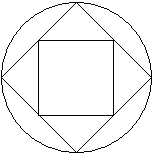
\includegraphics{PicJointSlides/8-hedrite8-1.pdf}}\par
$D_{4d}$ \textcolor{blue}{$8_{18}$} $(16)$
\end{minipage}
\begin{minipage}[b]{23mm}
\centering
\resizebox{19mm}{!}{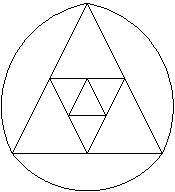
\includegraphics{PicJointSlides/8-hedrite9_1.pdf}}\par
$D_{3h}$ \textcolor{blue}{$9_{40}$} $(18)$\\
(Herschel)$^{*}$
\end{minipage}
\begin{minipage}[b]{23mm}
\centering
\resizebox{19mm}{!}{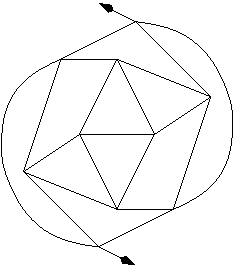
\includegraphics{PicJointSlides/8-hedrite10_1sec.pdf}}\par
%\resizebox{19mm}{!}{\rotatebox{90}{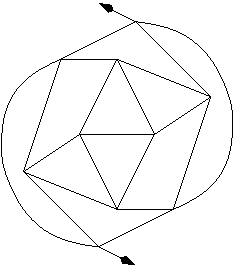
\includegraphics{PicJointSlides/8-hedrite10_1sec.pdf}}}\par
$D_{2}$ 
\textcolor{blue}{$10^2_{56}$} 
 $(6;14)$
\end{minipage}
\end{center}
Above links/knots  are given in \textcolor{blue}{Rolfsen, 1976 and 1990}, 
 notation.

Herschel graph:
% $APrism_3^2$:  
smallest non-Hamiltonian polyhedral 
 graph.
\end{frame}

\begin{frame}\frametitle{First four $(\{2,3\},6)$- and
$(\{1, 3\},6)$-spheres}
\vspace{-2.5mm}

\begin{center}
\begin{minipage}[b]{26mm}
\centering
\resizebox{22mm}{!}{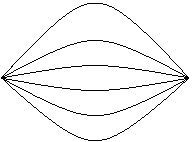
\includegraphics{PicJointSlides/Bundle6.pdf}}\par
$D_{6h}$ ($2^3$)
\end{minipage}  
\begin{minipage}[b]{23mm}
\centering
\resizebox{19mm}{!}{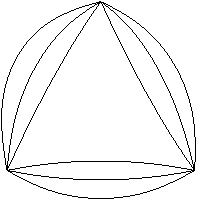
\includegraphics{PicJointSlides/Example23_6val_1.pdf}}\par
$D_{3h}$ ($3;6$)
\end{minipage}
\begin{minipage}[b]{24mm}
\centering
\resizebox{20mm}{!}{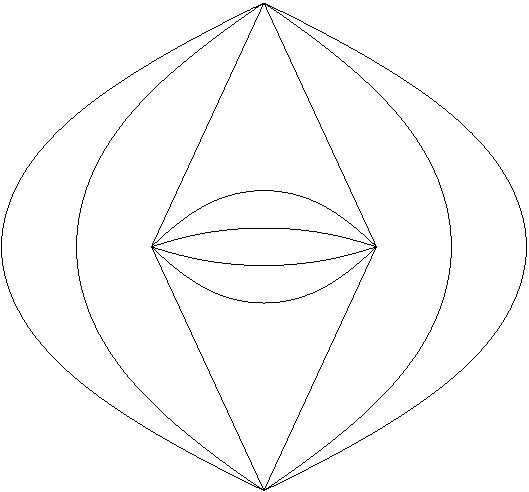
\includegraphics{PicJointSlides/23graph_3R2_2.pdf}}\par
$D_{2d}$ ($2^2;8$)
\end{minipage}
\begin{minipage}[b]{23mm}
\centering
\resizebox{19mm}{!}{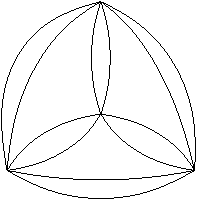
\includegraphics{PicJointSlides/Example23_6val_2.pdf}}\par
$T_{d}$ ($3^4$)
\end{minipage}
\end{center}



\begin{center}
\begin{minipage}[b]{25mm}
\centering
\resizebox{20mm}{!}{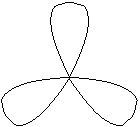
\includegraphics{PicJointSlides/Class_C3_C3vB.pdf}}\par
$C_{3v}$  ($3$)
\end{minipage} 
\begin{minipage}[b]{25mm}
\centering
\resizebox{17mm}{!}{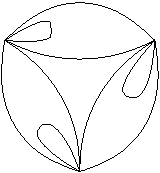
\includegraphics{PicJointSlides/Singular13_3vert.pdf}}\par
$C_{3h}$ ($3;6$)
\end{minipage}
\begin{minipage}[b]{25mm}
\centering
\resizebox{18mm}{!}{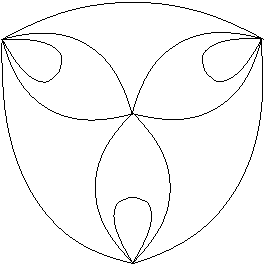
\includegraphics{PicJointSlides/Class_C3_C3v.pdf}}\par
%\resizebox{20mm}{!}{\rotatebox{90}{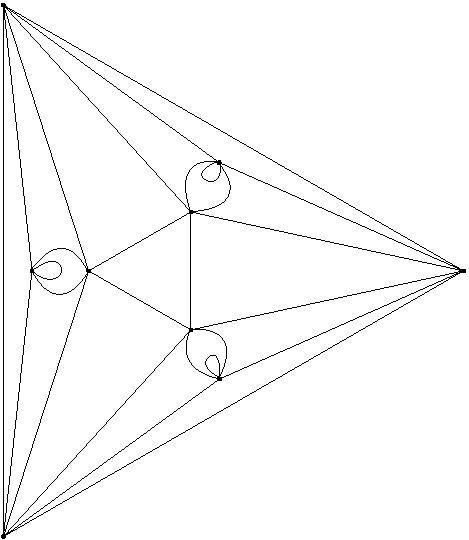
\includegraphics{PicJointSlides/PLdual9_sec.pdf}}}\par
$C_{3v}$ ($6^2$)
\end{minipage}
\begin{minipage}[b]{25mm}
\centering
%\resizebox{18mm}{!}{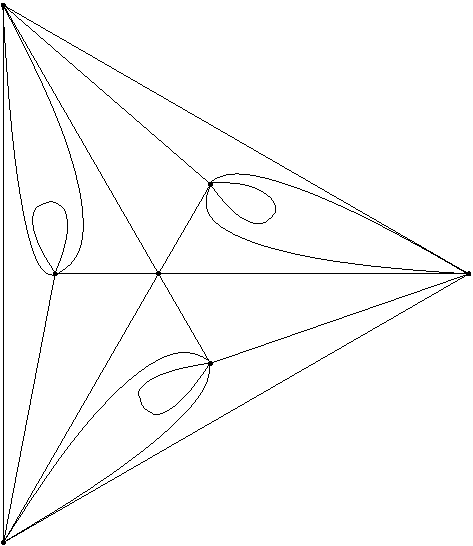
\includegraphics{PicJointSlides/Class_C3_C3_sec.pdf}}\par
\resizebox{20mm}{!}{\rotatebox{90}{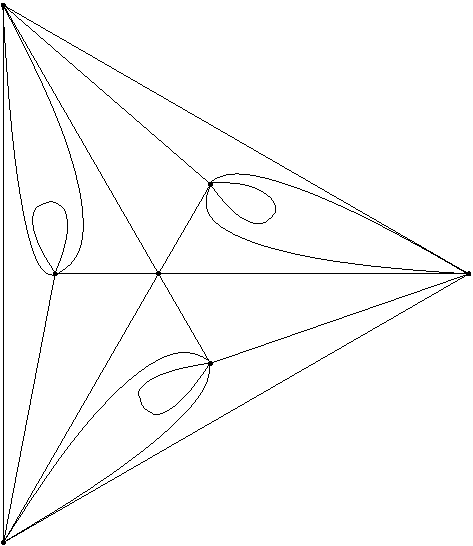
\includegraphics{PicJointSlides/Class_C3_C3_sec.pdf}}}\par
$C_{3}$  ($21$)
\end{minipage} 
\end{center}


%\textcolor{blue}{Gr\H{u}nbaum-Zaks, 1974}: $\{1,3\}_v$ exists iff
%$v=k^2+kl+l^2$ for integers $0\le l\le k$.We show that the number of
 % $\{1,3\}_v$'s is the number  of such representations of $v$, i.e. found
 %$GC_{k,l}(\{1,3\}_1)$.
\end{frame}


\section[]{Listing of $(\{a,b\};k)$-spheres with small $p_b$}

\frame{
\begin{center}
\begin{tabular*}{7cm}{c}
\\[-0.5cm]
{\Huge 
%\textcolor{blue}{III. }
\textcolor{red}{ 
$(\{a,b\};k)$-spheres}}
\\[4mm]{\Huge \textcolor{red}{
with  $p_b\le 3$: listings} }
\end{tabular*}
\end{center}}


\begin{frame}\frametitle{$(\{a,b\};k)$-spheres with  
\textcolor{red}{$p_b\le 2$}$<a<b$}
\vspace{-3.5mm}

\begin{itemize}
\item 
Remind:
$(a,k)$=$(3,3),(4,3),(3,4),(5,3), (3,5)$ if $k,a\ge 3$.

\item 
The only $(\{a,b\};k)$-spheres with \textcolor{red}{$p_b\le 1$} are 
$5$  \textcolor{blue}{Platonic $(a^k)$}:

Tetrahedron, Cube ($Prism_4$), Octahedron ($APrism_3$), Dodecahedron (snub 
$Prism_5$), Icosahedron (snub $APrism_3$). 

\item  
There exists unique \textcolor{blue}{trivial}
$3$-connected $(\{a,b\};k)$-sphere with \textcolor{red}{$p_b$=$2$} 
for
$(\{4,b\},3)$-, $(\{3,b\},4)$-,  $(\{5,b\},3)$-,
$(\{3,b\},5)$-:

$D_{bh}$ \textcolor{blue}{$Prism_b$}  and $D_{bd}$  
\textcolor{blue}{$APrism_b$}, 
\textcolor{blue}{snub $Prism_b$}, \textcolor{blue}{snub $APrism_b$}:   

two
$b$-gons separated by $b$-ring
of $4$-gons, $2b$-ring
of $3$-gons, 

two $b$-rings of $5$-gons, two $3b$-rings of $3$-gons.
%Doubled $b$-gon $D_{bh}$ is such $(\{2,b\},4)$-sphere.


\item 
Also, for $t$$\ge$$2$, 
 $10$ 
\textcolor{blue}{non-trivial}  $(\{a,at\};k)$-spheres with 
\textcolor{red}{$p_{at}$=$2$}:
%See below all such $(\{a,2a\},3)$-spheres, each 
%of symmetry $D_{2h}$.
%$(a,k)$=$(3,3),(3,4),(4,3),(3,5),(5,3)$,
%there is unique only $2$-connected such sphere ($D_{2h}$) 
%iff $b\equiv 0\,(mod\,a)$.
%divides $b$.
%\pause

$5$ 
%$2$-edge-connected 
$(\{a,ta\};k)$-spheres are ($D_{th}$)
\textcolor{red}{necklaces} of polycycles $\{a^k\}$-$e$;

 $3$ are ($D_{th}$)  \textcolor{red}{necklaces} of $t$ $v$-split
$\{3^4\}$ and $e$-split
 $\{5^3\}$, $\{3^5\}$;                              

 $(\{3,3t\},5)$-spheres $C_{th}$, $D_t$
are \textcolor{red}{necklaces} of $t$ $v$-, $f$-split $\{3^5\}$.
\end{itemize}
\end{frame}

\begin{frame}\frametitle{$(\{a,b$=$ta\};k)$-spheres with
\textcolor{red}{$p_{b}$=$2$}$<a$, $k$=$3,4,5$; case $t$=$2$}
\vspace{-3.5mm}
\begin{center}
%\hspace{-5mm}
\begin{minipage}[b]{16mm}
\centering
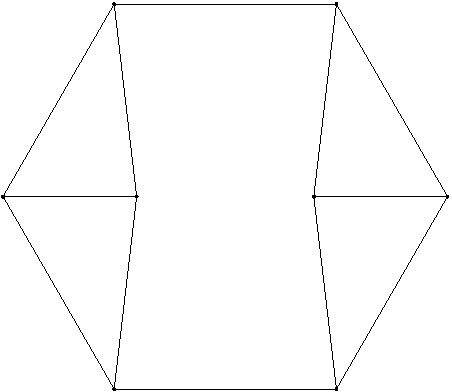
\epsfig{height=15mm, file=NanodiskPicture/3reg_PB2/3reg_a3_b6_sec.pdf}\par
$D_{2h}$: $a$=$3$
\end{minipage}
\hspace{1mm}
\begin{minipage}[b]{16mm}
\centering
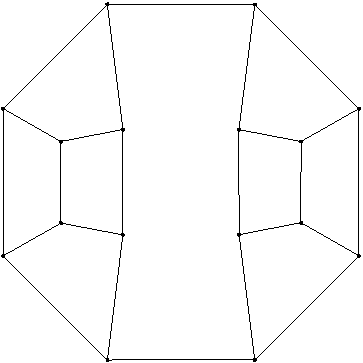
\epsfig{height=16mm, file=NanodiskPicture/3reg_PB2/3reg_a4_b8_sec.pdf}\par
 $a$=$4$
\end{minipage}  
\begin{minipage}[b]{16mm}
\centering
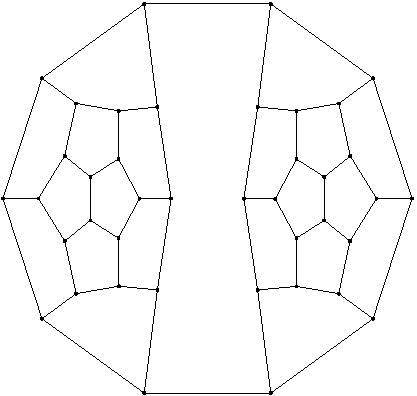
\epsfig{height=16mm, 
file=NanodiskPicture/3reg_PB2/3reg_a5_b10_b_sec.pdf}\par
$a$=$5$
\end{minipage}
\begin{minipage}[b]{16mm}
\centering
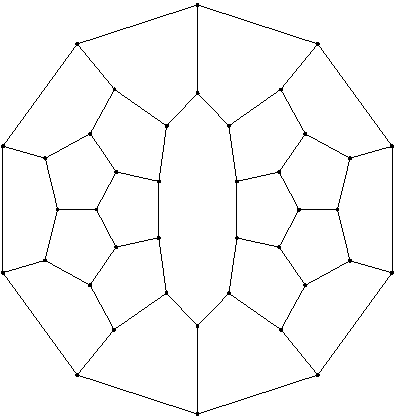
\epsfig{height=16mm, 
file=NanodiskPicture/3reg_PB2/3reg_a5_b10_a_sec.pdf}\par
$a$=$5$
\end{minipage}
\end{center}


\begin{center}
\begin{minipage}[b]{17mm}
\centering
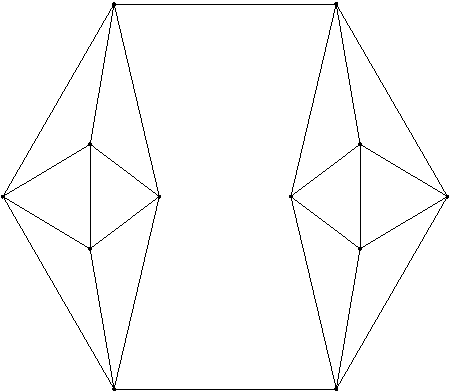
\epsfig{height=16mm, file=NanodiskPicture/4reg_PB2/4reg_a3_b6_aSec.pdf}\par
$a$=$3$ $D_{2h}$
\end{minipage}
\begin{minipage}[b]{17mm}
\centering
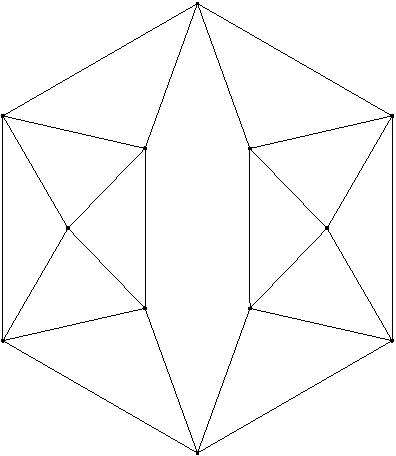
\epsfig{height=17mm, file=NanodiskPicture/4reg_PB2/4reg_a3_b6_bSec.pdf}\par
%$k$=$4$, 
$a$=$3$ $D_{2h}$
\end{minipage}  
\end{center}
%\vspace{-2mm}
%\end{frame}

\begin{center}
\begin{minipage}[b]{17mm}
\centering
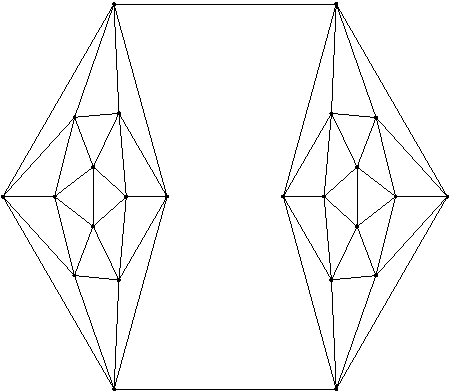
\epsfig{height=15mm, file=NanodiskPicture/5reg_PB2/PL3b_sec.pdf}\par
$a$=$3$ $D_{2h}$
\end{minipage}
\begin{minipage}[b]{17mm}
\centering
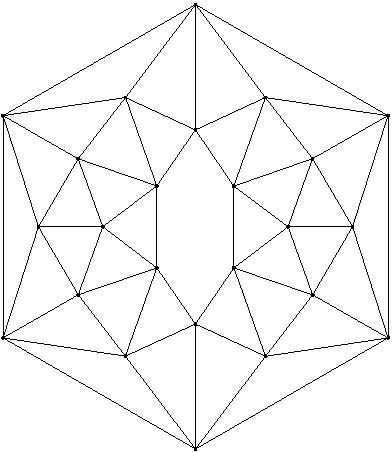
\epsfig{height=16mm, file=NanodiskPicture/5reg_PB2/PL_D2h_b2_sec.pdf}\par
%$k$=$5$ 
$a$=$3$ $D_{2h}$
\end{minipage}  
\begin{minipage}[b]{17mm}
\centering
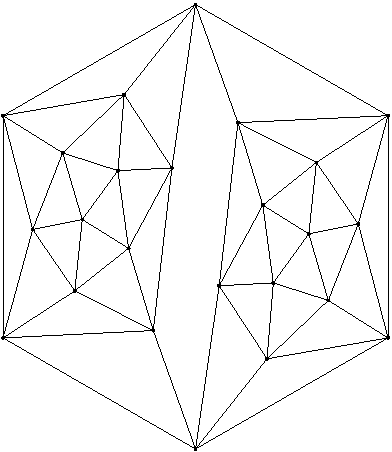
\epsfig{height=16mm, file=NanodiskPicture/5reg_PB2/PL10_sec.pdf}\par
%$k$=$5$ 
$a$=$3$ $C_{2h}$
\end{minipage}
\begin{minipage}[b]{17mm}
\centering
\epsfig{height=16mm, file=NanodiskPicture/5reg_PB2/PL_dcdSec.pdf}\par
$a$=$3$ $D_{2}$
\end{minipage}
\end{center}
\end{frame}

\begin{frame}\frametitle{Proof method: elementary $(a,k)$-polycycles}
\vspace{-3.5mm}
\begin{itemize}
\item A \textcolor{red}{$(a,k)$-polycycle} is a
$2$-connected plane graph with faces partitioned
in  $a$-gonal
%two families: $F_1$  (
\textcolor{blue}{proper  faces} and 
%$F_2$ 
%(pairwisely disjoint 
\textcolor{blue}{holes}, exterior face among them, 
so that
vertex degrees are  in $\{2,\dots ,k\}$ and  can be  $<k$
only for a  vertex lying on the
boundary of a hole.
\item Any $(a,k)$-polycycle \textcolor{red}{decomposes uniquely} along 
its \textcolor{blue}{bridges} (non-boundary  going   
hole-to-hole, possibly, same, edges)

into  \textcolor{red}{elementary} ones. Cf. integer factorisation into 
primes.  
\item We listed them for $\kappa_a$=$1$+$\frac{a}{k}-\frac{a}{2}$$\ge$$0$. Othervise, 
continuum.
\end{itemize}

\begin{center}
\hspace{-26mm}
\begin{minipage}[b]{20mm}
\centering
\epsfig{height=19mm, file=PicJointSlides/PL5_15_5_Cs_exmpB.pdf}\par
\end{minipage}
\end{center} 
This $(\{5,15\},3)$-sphere with $p_{15}$=$3$ 
is a $3$-holes $(\{5\},3)$-polycycle 

It decomposes into five
$1$-hole elementary $(\{5\};k)$-polycycles.

\end{frame} 



\begin{frame}\frametitle{$(\{a,b\},3)$-spheres with
$\textcolor{red}{p_b=3}$$\le a$}
\vspace{3mm}
\begin{itemize}

\item   $(\{a,b\};k)$-sphere with \textcolor{red}{$p_b=3$}$\le a$ exists
if and only if
$b\equiv 2,a,2a-2 \pmod{2a}$ and  $b\equiv 4,6 \pmod{10}$
if $a$=$5$.
 

\item There are $7$ such spheres with $t$=$\lfloor{\frac{b}{6}}\rfloor$=$0$
and 

$3$+$4$+$5$+$17$ of them for any $t\ge 1$.
\item  Such sphere are unique if $b$ is not
$\equiv a \pmod{2a}$ and then their symmetry is $D_{3h}$, except
%D_3$ if 
% when
$(a,k)=(3,5)$,
 when it is $D_3$.
 



\end{itemize}

\begin{center}
\begin{minipage}[b]{19mm}
\centering
\resizebox{16mm}{!}{\includegraphics{PicJointSlides/GC20Bundle.pdf}}\par
8, $D_{3h}$\\
$(\{2,6\};3)$-
$\vec{p}$=$(3,3)$
\end{minipage}
\begin{minipage}[b]{19mm}
\centering
%\resizebox{20mm}{!}{\includegraphics{PicJointSlides/First4nD3hthi.pdf}}\par
\resizebox{19mm}{!}{\rotatebox{90}{\includegraphics{PicJointSlides/First4nD3hthi.pdf}}}\par
14, $D_{3h}$\\
 $(\{4,6\};3)$-
  $\vec{p}$=$(6,3)$ 
 \end{minipage}
 \begin{minipage}[b]{19mm}
\centering
\resizebox{19mm}{!}{\includegraphics[bb=1 1 457 464,
clip]{PicJointSlides/Picture2.pdf}}\par
26,  $D_{3h}$\\ $(\{5,6\};3)$- 
%($12^3;42_{0,9}$)
$\vec{p}$=$(12,3)$\end{minipage}
\begin{minipage}[b]{19mm}
\centering
\resizebox{19mm}{!}{\includegraphics{PicJointSlides/8-hedrite9_1.pdf}}\par
9, $D_{3h}$ \\
 $(\{3,4\};4)$-
 $\vec{p}$=$(8,3)$\end{minipage}
  %\end{center}
\begin{minipage}[b]{20mm}
\centering
\epsfig{height=20mm, file=PicJointSlides//PLico_exp.pdf}\par
 18, $D_{3}$\par
 $(\{3,4\};5)$-
 $\vec{p}$=$(26,3)$ \end{minipage} 
 
 
 \end{center}
 \end{frame}     


\begin{frame}\frametitle{$(\{a,b\},k)$-spheres with $a=1,2$ and 
$p_b=1$}
%\vspace{-3mm}
\begin{itemize}

\item
There are no
 %the inequality $p_a,p_b\neq 1$ holds for any  
 $(\{a,b\};k)$-spheres
 %$\mathbb{S}^2$ 
 with $a\ge 2$, having  $p_b= 1$.
 \item  
The only  $(\{1,b\};k)$-spheres
%$\mathbb{S}^2$ 
 with $p_b$=$1$ are:
 
$1$-vertex \textcolor{red}{$b$-foliums} ($K_1$ with $b$ $1$-gons); so,  $k$=$2b$$\ge$$ 4$, $p_1$=$b$ and

$2$-vertex \textcolor{red}{$b$-dumbbells} ($K_2$ with $\frac{b-2}{2}$ $1$-gons on each vertex); so,
having  odd $k$=$b-1$$\ge$$ 3$ and  $p_1$=$b-2$.

 $2$-folium and  $4$-dumbbell are  elliptic,   $3$-folium is 
parabolic. 
%Others: hyperbolic
\end{itemize}

\begin{center}
\begin{minipage}[b]{25mm}
\centering
\resizebox{20mm}{!}{\includegraphics{PicJointSlides/Class_C3_C3vB.pdf}}\par
%$C_{3v}$  
$3$-folium
\end{minipage} 

\end{center}

\end{frame}  

\begin{frame}\frametitle{$(\{a,b\},k)$-spheres with $a=1,2$ and 
$p_b= 2$}
\vspace{-3mm}
\begin{itemize}

\item

%(2) and (1) imply that a
An $(\{2,b\};k)$-$\mathbb{S}^2$ with $p_b$=$2$ exists if and only if $bk$ is even, and then it has  
%$b$ vertices, $b\ge 3\le k$ and $p_2=\frac{b(k-2)}{2}$. Such spheres exist for any integers
 %$b,k\ge 3$ with 
% integer 
$\vec{p}$=$(\frac{b(k-2)}{2},2)$ and $v$=$b$ vertices. It is either,
%It is lego-like if and only if it is lego-admissible, i.e., $p_2$ is even.
%All $(\{2,b\};k)$-$\mathbb{S}^2$ with $p_b=2$ are: 

\textcolor{blue}{for odd $b$}, $b$-cycle with edges repeated $\frac{k}{2}$ times; 

or, \textcolor{blue}{for even $b$}  and any integer $m\in [1,\frac{k}{2}]$,
$b$-cycle with edges repeated, alternatively, $m$ and $k-m$ times.

 
\item
 %(2) and (1) imply that a
 An $(\{1,b\};k)$-sphere with $p_b$=$2$ exists iff  $v$=$\frac{4b}{k+2}$$\in $$\mathbb{N}$, and then it has
  %$\frac{4b}{k+2}$ vertices, $b\ge 2< k$ and integer 
  $v$ vertices and
$\vec{p}$=$(2(b-v),2)$. It is either,
%It is  lego-admissible and, among all with given $(b,k)$, there exists a lego-like one. 
  %All $(\{1,b\};k)$-$\mathbb{S}^2$ with $p_b=2$  are: 
 

\textcolor{blue}{for $k=3$},  a $\frac{2b}{5}$-cycle with  matches from  each cycle's vertex, 
so that
the same  number of them
%$1$-gons 
goes inside and outside.
%going inside for the half of them
%and outside for other half;

or, \textcolor{blue}{for $k\ge 4$},  a $\frac{4b}{k+2}$-cycle with  $\frac{k-2}{2}$ $1$-gons  from each  vertex, so that
the same  number of them
%$1$-gons 
goes inside and outside.


\end{itemize}
\small
\begin{center}
\begin{minipage}[b]{19mm}
\centering
\resizebox{13mm}{!}{\includegraphics{PicJointSlides/4-hedrite4_1.pdf}}\par
4, $D_{4h}$ 
$(\{2, 4\};4)$-
$\vec{p}$=$(4,2)$
\end{minipage}
\begin{minipage}[b]{20mm}
\centering
\resizebox{20mm}{!}{\includegraphics{PicJointSlides/4-hedrite4-2.pdf}}\par
4, $D_{2h}$ 
$(\{2, 4\};4)$-
$\vec{p}$=$(4,2)$
\end{minipage}
\hspace{1mm}
\begin{minipage}[b]{19mm}\centering
\epsfig{height=13mm, file=Map15_3_22.eps}\par
4, $C_{2h}$
%$D_{2d}$
$(\{1, 5\};3)$-
$\vec{p}$=$(2,2)$
\end{minipage}
\hspace{8mm}
\begin{minipage}[b]{19mm}\centering
\epsfig{height=13mm, file=Map13_4_22.eps}\par
2, $C_{2h}$
%$D_{2d}$\\
$(\{1, 3\};4)$-
$\vec{p}$=$(2,2)$
\end{minipage}
%\hspace{3mm}
\end{center}


\end{frame}  

\section[]{Symmetry groups of $(\{a,b\};k)$-spheres}

\frame{
\begin{center}
\begin{tabular*}{7cm}{c}
\\[-0.5cm]
{\Huge 
%\textcolor{blue}{V. }
\textcolor{red}{Symmetry groups  of}}
\\[4mm]{\Huge \textcolor{red}{$(\{a,b\};k)$-spheres}
}
\end{tabular*}
\end{center}
}



\begin{frame}\frametitle{Finite isometry groups}
\vspace{-1mm}


All finite groups of isometries of $3$-space $\mathbb{E}^3$ are 
classified. 

In Schoenflies notations, they are:
\begin{itemize}
\item $C_1$ is the \textcolor{blue}{trivial} group
\item $C_s$ is the group generated by a \textcolor{blue}{plane reflexion}
\item $C_i=\{I_3, -I_3\}$ is the \textcolor{blue}{inversion} group
\item $C_m$ is the group generated by a \textcolor{blue}{rotation} of 
order 
$m$ of axis $\Delta$
\item $C_{mv}$ ($\simeq$ dihedral group) is the group generated by $C_m$ 
and $m$ \textcolor{blue}{reflexion containing} $\Delta$
\item $C_{mh}=C_m\times C_s$ is the group generated by $C_m$ and the 
\textcolor{blue}{symmetry by the plane orthogonal} to $\Delta$
\item $S_{2m}$ is the group of order $2m$ generated by an 
\textcolor{blue}{antirotation}, i.e. commuting composition of a rotation
and a plane symmetry
\end{itemize}
\end{frame}





\begin{frame}\frametitle{Finite isometry groups $D_m$, $D_{mh}$, $D_{md}$}

\begin{itemize}
\item $D_m$ ($\simeq$ dihedral group) is the group generated of $C_m$ and 
$m$ \textcolor{blue}{rotations of order $2$
with axis orthogonal} to $\Delta$
\item $D_{mh}$ is the group generated by $D_m$ and a 
\textcolor{blue}{plane symmetry orthogonal} to
$\Delta$
\item $D_{md}$ is the group generated by $D_m$ and $m$ 
\textcolor{blue}{symmetry planes containing}
$\Delta$ and which \textcolor{blue}{does not contain} axis of order $2$
\end{itemize}
%\pause

\begin{center}
\begin{minipage}{3.9cm}
\centering
\resizebox{3.8cm}{!}{\includegraphics{PicJointSlides/D2h.pdf}}\par
$D_{2h}$
\end{minipage}
\begin{minipage}{3cm}
\centering
\resizebox{2.7cm}{!}{\includegraphics{PicJointSlides/D2d.pdf}}\par
$D_{2d}$
\end{minipage}
\end{center}    


\end{frame}





\begin{frame}\frametitle{Remaining $7$ finite isometry groups}
\vspace{-1mm}
\begin{itemize} 
\item $I_h=H_3$ is the group of
\textcolor{blue}{isometries} of \textcolor{blue}{Dodecahedron};
$I_h\simeq Alt_5\times C_2$ 
\item $I\simeq Alt_5$ is the group of \textcolor{blue}{rotations} of 
Dodecahedron
\item $O_h=B_3$ is the group of \textcolor{blue}{isometries} of 
\textcolor{blue}{Cube}
\item $O\simeq Sym(4)$ is the group of \textcolor{blue}{rotations} of Cube
\item $T_d=A_3\simeq Sym(4)$ is the group of \textcolor{blue}{isometries}
of  \textcolor{blue}{Tetrahedron}
\item $T\simeq Alt(4)$ is the group of \textcolor{blue}{rotations} of Tetrahedron
\item $T_h=T\cup -T$
\end{itemize}
\vspace{1.5mm}
%\pause 

While 
(point group) $Isom(P)\subset Aut(G(P))$ (combinatorial group),
%{\em {\bf Theorem} (
\textcolor{blue}{Mani, 1971}:
for any  $3$-polytope $P$, there is a map-isomorphic $3$-polytope $P'$ 
(so, with the same 
skeleton $G(P')=G(P)$), such that the    
group $Isom(P')$ of its isometries  is isomorphic to $Aut(G)$.
\end{frame}





\begin{frame}\frametitle{$8$ parabolic families: symmetry  groups}
\vspace{-2mm}

\begin{enumerate}
\item
%[\ding{108}] 
$28$ for \textcolor{red}{$\{5,6\}_v$}:  
$C_1$, $C_s$, $C_i$; $C_2$, $C_{2v}$, $C_{2h}$, $S_4$; $C_3$,
$C_{3v}$, $C_{3h}$, $S_6$; $D_2$, $D_{2h}$, $D_{2d}$; $D_3$,  
$D_{3h}$, $D_{3d}$; $D_5$, $D_{5h}$, $D_{5d}$; $D_6$, $D_{6h}$,
$D_{6d}$; $T$, $T_d$, $T_h$; $I$, $I_h$ 
(\textcolor{blue}{Fowler--Manolopoulos, 1995})
\item
%[\ding{108}]  
$16$ for \textcolor{red}{$\{4,6\}_v$}: $C_1$, $C_s$,
$C_{i}$; $C_2$, $C_{2v}$, $C_{2h}$; $D_2$, $D_{2h}$, $D_{2d}$; $D_3$,
$D_{3h}$, $D_{3d}$; $D_6$, $D_{6h}$; $O$, $O_h$
(\textcolor{blue}{Deza--Dutour,  2005})
\item
%[\ding{108}]  
$5$ for \textcolor{red}{$\{3,6\}_v$}: $D_{2}$,
$D_{2h}$, $D_{2d}$; $T$, $T_d$ (\textcolor{blue}{Fowler--Cremona,1997})
\item
%[\ding{108}]  
$2$ for \textcolor{red}{$\{2, 6\}_v$}: $D_3$, $D_{3h}$ 
(\textcolor{blue}{Gr\H{u}nbaum--Zaks, 1974})
%\pause
\item
%[\ding{108}]  
$18$ for \textcolor{red}{$\{3, 4\}_v$}: $C_{1}$, $C_s$,
$C_i$; $C_2$, $C_{2v}$, $C_{2h}$, $S_4$; $D_2$, $D_{2h}$, $D_{2d}$;
$D_3$, $D_{3h}$, $D_{3d}$; $D_4$,
$D_{4h}$, $D_{4d}$; $O$, $O_h$   
(\textcolor{blue}{Deza-Dutour-Shtogrin, 2003})
\item
%[\ding{108}]  
$5$ for \textcolor{red}{$\{2, 4\}_v$}: $D_2$, $D_{2h}$, 
$D_{2d}$; $D_4$, $D_{4h}$, all in $[D_2,D_{4h}]$ (\textcolor{blue}{same})
%\pause
\item
%[\ding{108}] 
$3$ for \textcolor{red}{$\{1, 3\}_v$}:  $C_3$,
$C_{3v}$,  $C_{3h}$ (\textcolor{blue}{Deza--Dutour,  2010})
\item
%[\ding{108}]  
$22$ for \textcolor{red}{$\{2, 3\}_v$}: $C_1$, 
$C_s$, $C_i$; $C_2$, $C_{2v}$, $C_{2h}$,  $S_4$; $C_3$,
$C_{3v}$, $C_{3h}$, $S_6$; $D_2$, $D_{2h}$, $D_{2d}$; $D_3$,
$D_{3h}$, $D_{3d}$; $D_6$, $D_{6h}$; $T$, $T_d$, $T_h$ 
(\textcolor{blue}{same}) 
%\item 
\end{enumerate}
$38$ for  \textcolor{red}{icosahedrites $(\{3,4\},5)$-} 
(\textcolor{blue}{same, 2011}).
%\end{enumerate}
\end{frame}



\begin{frame}\frametitle{$8$ families: 
Goldberg--Coxeter construction  $GC_{k,l}(.)$}
\vspace{-2mm}
With
%Agregating  groups 
\textcolor{red}{${\bf T}$}=$\{T,T_d,T_h\}$, \textcolor{red}{${\bf O}$}=$\{O,O_h\}$,
\textcolor{red}{${\bf I}$}=$\{I,I_h\}$,
\textcolor{red}{${\bf C_1}$}=$\{C_1,C_s,C_i\}$,  
\textcolor{red}{${\bf C_m}$}=$\{C_m,C_{mv},C_{mh},S_{2m}\}$, 
 \textcolor{red}{${\bf D_m}$}=$\{D_m,D_{mh},D_{md}\}$,  
we get
\begin{enumerate}
\item
%[\ding{108}] 
for \textcolor{red}{$(\{5,6\},3)$-}:
${\bf C_1}$,  ${\bf C_2}$, ${\bf C_3}$,  ${\bf D_2}$,  ${\bf D_3}$, ${\bf 
D_5}$,  ${\bf D_6}$, ${\bf T}$,  \textcolor{blue}{${\bf I}$}
\item
%[\ding{108}]   
for \textcolor{red}{$(\{2, 3\},6)$-}: ${\bf C_1}$,
${\bf C_2}$, ${\bf C_3}$, ${\bf D_2}$, ${\bf D_3}$,
\textcolor{blue}{$\{D_6,D_{6h}\}$}, \textcolor{blue}{${\bf T}$}
\item
%[\ding{108}]   
for \textcolor{red}{$(\{4,6\},3)$-}: ${\bf C_1}$, 
${\bf C_2}$$\setminus$$ S_{4}$, ${\bf D_2}$, ${\bf 
D_3}$,  \textcolor{blue}{$\{D_6,D_{6h}\}$}, \textcolor{blue}{${\bf O}$}
\item
%[\ding{108}]  
for \textcolor{red}{$(\{3, 4\},4)$-}: ${\bf C_{1}}$,
${\bf C_2}$,  ${\bf D_2}$,
${\bf D_3}$, ${\bf D_4}$, \textcolor{blue}{${\bf O}$}
\item
%[\ding{108}]  
for \textcolor{red}{$(\{3,6\},3$-}: ${\bf D_{2}}$, 
\textcolor{blue}{$\{T,T_d\}$} 
%\item[\ding{108}]  for \textcolor{red}{$(\{2, 6\},3)$-}: 
\textcolor{blue}{$\{D_3,D_{3h}\}$}
%\item[\ding{108}]  for \textcolor{red}{$(\{3, 4\},4)$-}: ${\bf C_{1}}$, 
%${\bf C_2}$,  ${\bf D_2}$, ${\bf D_3}$, ${\bf D_4}$, \textcolor{blue}{${\bf O}$}
\item
%[\ding{108}]  
for \textcolor{red}{$(\{2, 4\},4)$-}: ${\bf D_2}$,  
\textcolor{blue}{$\{D_4,D_{4h}\}$}
%\item[\ding{108}]   for \textcolor{red}{$(\{2, 3\},6)$-}: ${\bf C_1}$,
%${\bf C_2}$, ${\bf C_3}$, ${\bf D_2}$, ${\bf D_3}$, 
%\textcolor{blue}{$\{D_6,D_{6h}\}$}, \textcolor{blue}{${\bf T}$}
\item
%[\ding{108}]  
for \textcolor{red}{$(\{2, 6\},3)$-}: 
${\bf D_3}$$\setminus$$ D_{3d}$=
\textcolor{blue}{$\{D_3,D_{3h}\}$}
\item
%[\ding{108}] 
for \textcolor{red}{$(\{1, 3\},6)$-}:
${\bf C_3}$$\setminus$$ S_{6}$=\textcolor{blue}{$\{C_3,
C_{3v},C_{3h}\}$}
%\item 
\end{enumerate}
if  \textcolor{red}{$(\{3,4\},5)$-}:
${\bf C_1}$,  ${\bf C_2}$, ${\bf C_3}$,  ${\bf C_4}$, ${\bf C_5}$, ${\bf D_2}$,  
${\bf D_3}$, ${\bf
D_4}$,  ${\bf D_5}$, ${\bf T}$,  ${\bf O}$, ${\bf I}$.


%\end{enumerate}
%\vspace{1mm}
\pause

Spheres of blue symmetry  are  $GC_{k,l}$ from 1st such; so, given
 by one complex (Gaussian for $k$=$4$, Eisenstein for $k$=$3,6$) 
parameter.

%There are $O(v)$ of  such  $1$-parametrized  $\le v$-vertex spheres.

\textcolor{blue}{Goldberg, 1937} and \textcolor{blue}{Coxeter, 1971}: 
$\{5,6\}_v(I,I_h)$, $\{4,6\}_v(O,O_h)$,  
$\{3,6\}_v(T,T_d)$. 
\textcolor{blue}{Dutour-Deza, 2004 and  2010}: for other cases.
\end{frame}

\section[]{Goldberg--Coxeter construction
and parameterizing}

\frame{
\begin{center}
\begin{tabular*}{7cm}{c}
\\[-0.5cm]
{\Huge 
%\textcolor{blue}{VI. }
\textcolor{red}{Goldberg--Coxeter}}
\\[4mm]{\Huge \textcolor{red}{construction and}}
\\[4mm]{\Huge \textcolor{red}{parameterizing}
}
\end{tabular*}
\end{center}
}




\begin{frame}\frametitle{Goldberg--Coxeter ($1$ parameter) construction $GC_{k,l}(.)$}
\vspace{-2.5mm}
\begin{itemize}
\item Take a $3$- or $4$-regular plane graph $G$. The faces of dual graph 
$G^{*}$ are triangles or squares, respectively.
\item Break each face
% triangles or squares 
into pieces according to parameter 
$(k,l)$.

{\em Master polygons}
below have area $\cal{A}$$(k^2$+$kl$+$l^2)$ or $\cal{A}$$(k^2$+$l^2)$, where  $\cal{A}$ is the area of 
 a small 
polygon.
\end{itemize}
\begin{center}
\resizebox{9.0cm}{!}{\includegraphics{PicJointSlides/GoldbergBreakdown.pdf}}
\end{center}

\end{frame}
\begin{frame}\frametitle{Gluing the pieces together in a coherent way}
\vspace{-2.5mm}
\begin{itemize}
\item Gluing the pieces so that, say, $2$ non-triangles, coming from  
subdivision 
of neighboring triangles, form a small triangle,
%\item 
we obtain 
another \textcolor{blue}{triangulation} or 
\textcolor{blue}{quadrangulation} of the plane.
\end{itemize}
\begin{center}
\centering
\resizebox{3.8cm}{!}{\includegraphics{PicJointSlides/MergingBreakdown2.pdf}}
\end{center}   
\begin{itemize} 
\item The dual is  a $3$- or $4$-regular plane graph,  
 denoted $GC_{k,l}(G)$; we call it \textcolor{red}{Goldberg--Coxeter construction}.
\item It 
%The construction 
works for \textcolor{blue}{any} $3$- or $4$-regular  map on 
\textcolor{blue}{oriented surface}.
\end{itemize}  
\end{frame}

\begin{frame}\frametitle{$GC_{k,l}(Cube)$ for $(k,l)=(1,0),(1,1),(2,0),(2,1)$}
\vspace{-2.5mm}
\begin{center}
\begin{minipage}{3.8cm}
\centering
\resizebox{3.6cm}{!}{\includegraphics{PicJointSlides/Cube1_0-sec.pdf}}
\end{minipage}
\begin{minipage}{3.8cm}
\centering
\resizebox{3.6cm}{!}{\includegraphics{PicJointSlides/Cube1_1-sec.pdf}}
\end{minipage}
\begin{minipage}{3.8cm}
\centering
\resizebox{3.6cm}{!}{\includegraphics{PicJointSlides/Cube2_0-sec.pdf}}
\end{minipage}
\begin{minipage}{3.8cm}
\centering
\resizebox{3.6cm}{!}{\includegraphics{PicJointSlides/Cube2_1-sec.pdf}}
\end{minipage}
\end{center}
\end{frame}

\begin{frame}\frametitle{Goldberg--Coxeter construction from Octahedron}
\vspace{-2.5mm}
\begin{center}
\begin{minipage}{3.5cm}
\centering
\resizebox{3.1cm}{!}{\includegraphics{PicJointSlides/Octahedron1_0sec.pdf}}
\end{minipage}
\begin{minipage}{3.5cm}
\centering
\resizebox{3.1cm}{!}{\includegraphics{PicJointSlides/Octahedron1_1sec.pdf}}
\end{minipage}
\begin{minipage}{3.5cm}
\centering
\resizebox{3.1cm}{!}{\includegraphics{PicJointSlides/Octahedron2_0sec.pdf}}
\end{minipage}
\begin{minipage}{3.5cm}
\centering
\resizebox{3.1cm}{!}{\includegraphics{PicJointSlides/Octahedron2_1sec.pdf}}
\end{minipage}
\end{center}
\end{frame}

\begin{frame}\frametitle{The case $(k,l)$=$(1,1)$ of $GC_{k,l}(G)$}

\begin{center}
\begin{minipage}{4.6cm}
\centering
\resizebox{3.8cm}{!}{\includegraphics{PicJointSlides/ExampleLeapFrog3.pdf}}\par
For $3$-regular $G$=$(V,E)$, \par
$GC_{1,1}$ is called \textcolor{red}{leapfrog}
($\frac{1}{3}$-truncation of the dual),\par
$3|V|$ vertices.\\
Truncated Octahedron
\end{minipage}
\begin{minipage}{4.6cm}
\centering
\resizebox{3.8cm}{!}{\includegraphics{PicJointSlides/ExampleMedial3.pdf}}\par
\vspace{0.6cm} 
For  $4$-regular $G$=$(V,E)$, \par
$GC_{1,1}$ is called \textcolor{red}{medial}\par
($\frac{1}{2}$-truncation),\par
$|E|$ vertices\\
 Cuboctahedron
\end{minipage} 
\end{center} 

\end{frame}

\begin{frame}\frametitle{The case $(k,l)$=$(k,0)$ of $GC_{k,l}(G)$: $k$-inflation}
\vspace{-2.5mm}

%If  ZC-vector of $G$ is $\dots,c_i^{l_i},\dots$, then  ZC-vector
%of $GC_{k,0}(G)$ is $\dots,kc_i^{kl_i},\dots$. The case $(2,0)$ is 
 \textcolor{red}{Chamfering} ({\em quadrupling}) $GC_{2,0}(G)$  of smallest
 %$8$ 1st 
  $(\{a,b\};k)$-spheres,  
 $(a,b)$=$(2,6),(3,6),(4,6),(5,6)$ and $(2,4),(3,4),(1,3),(2,3)$,  are: 
\begin{center}
\begin{minipage}[b]{18mm}
\centering
\resizebox{16mm}{!}{\includegraphics{PicJointSlides/GC20Bundle.pdf}}\par
$D_{3h}$  ($12^2$)
\end{minipage}
\begin{minipage}[b]{26mm}
\centering
\resizebox{22mm}{!}{\includegraphics{PicJointSlides/ebe1.pdf}}\par
 $T_d$ $(8^6)$
\end{minipage}
\begin{minipage}[b]{23mm}
\centering
\resizebox{19mm}{!}{\includegraphics{PicJointSlides/ebe2.pdf}}\par
 $O_h$ $(12^8)$
\end{minipage}
\begin{minipage}[b]{25mm}
\centering
\resizebox{21mm}{!}{\includegraphics{PicJointSlides/C80Sec.pdf}}\par
 $I_h$ $(20^{12})$
\end{minipage}
\begin{minipage}[b]{26mm}
\centering
\resizebox{22mm}{!}{\includegraphics{PicJointSlides/4-hedrite8_3.pdf}}\par
 $D_{4h}$ $(4^{4})$
\end{minipage}
\begin{minipage}[b]{20mm}
\centering
\resizebox{16mm}{!}{\includegraphics{PicJointSlides/WCube02.pdf}}\par
 $O_h$ $(8^6)$
\end{minipage}
\begin{minipage}[b]{23mm}
\centering
\resizebox{16mm}{!}{\includegraphics{PicJointSlides/Class_C3_C3v.pdf}}\par
$C_{3v}$  ($6^2$)
\end{minipage}
\begin{minipage}[b]{20mm}
\centering
\resizebox{18mm}{!}{\includegraphics{PicJointSlides/23graph_3R2_1.pdf}}\par
$D_{6h}$  ($4^3,6^2$)
\end{minipage}


\end{center}  
%For $4$-regular $G$,   \textcolor{blue}{$GC_{2k^2,0}(G)$=$GC_{k,k}(GC_{k,k}(G))$} 
 %by $(k$+$ki)^2$=$2k^2i$.
\end{frame}

\begin{frame}\frametitle{First four $GC_{k,l}(4$$\times $$K_2)$ and   
$GC_{k,l}(6$$\times $$K_2)$}
\vspace{-2.5mm}


\begin{center}
\begin{minipage}[b]{25mm}
\centering
\resizebox{24mm}{!}{\includegraphics{PicJointSlides/4-hedrite2_1.pdf}}\par
$D_{4h}\,$ 
\textcolor{red}{$4$$\times $$K_2$}
\end{minipage}
\begin{minipage}[b]{23mm}
\centering
\resizebox{19mm}{!}{\includegraphics{PicJointSlides/4-hedrite4_1.pdf}}\par
$D_{4h}$ 
 \textcolor{blue}{medial} 
%$G_{1,1}$
\end{minipage}
\begin{minipage}[b]{21mm}
\centering
\resizebox{21mm}{!}{\includegraphics{PicJointSlides/4-hedrite8_3.pdf}}\par
$D_{4h}$  $G_{2,0}$
\end{minipage}
\begin{minipage}[b]{28mm}
\centering
\resizebox{22mm}{!}{\includegraphics{PicJointSlides/4-hedrite10_1sec.pdf}}\par
$D_{4}$ $G_{2,1}$
\end{minipage}   
\end{center}


\begin{center}
\begin{minipage}[b]{25mm}
\centering
\resizebox{21mm}{!}{\includegraphics{PicJointSlides/Bundle6.pdf}}\par
$D_{6h}\,$ \textcolor{red}{$6$$\times $$K_2$}
%($2^3$)
\end{minipage}
\begin{minipage}[b]{23mm}
\centering
%\resizebox{19mm}{!}{\includegraphics{PicJointSlides/SmallOcta_D3d}}\par
%\resizebox{18mm}{!}{\includegraphics{PicJointSlides/IcosahedronTh.pdf}}\par
\resizebox{19mm}{!}{\rotatebox{90}{\includegraphics{PicJointSlides/SmallOcta_D3d.pdf}}}\par
$D_{3d}$  $G_{1,1}$ 
%($3^2,4^3$)
\end{minipage}
\begin{minipage}[b]{21mm}
\centering
\resizebox{19mm}{!}{\includegraphics{PicJointSlides/23graph_3R2_1.pdf}}\par
$D_{6h}$  $G_{2,0}$ 
%($4^3,6^2$)
\end{minipage}
\begin{minipage}[b]{28mm}
\centering
\resizebox{22mm}{!}{\includegraphics{PicJointSlides/SmallestD6sec.pdf}}\par
$D_{6}$ $G_{2,1}$ 
%($14^3$)
\end{minipage}
\end{center}





\end{frame}
\begin{frame}\frametitle{First four $GC_{k,l}(3$$\times$$ K_2)$ and $GC_{k,l}(Trifolium =3$$\times$$(aa))$} 
%$GC_{kl}(\{1,3\}_1)$ for $(k,l)=(1,0)$,$(1,1)(2,0),(2,1)$}




All $(\{2,6\},3)$-spheres are $G_{k,l}(3$$\times$$ K_2)$:  $D_{3h}$, 
$D_{3h}$, $D_3$ if $l$=$0,k$, else.
\begin{center}
\begin{minipage}[b]{25mm}
\centering
\resizebox{21mm}{!}{\includegraphics{PicJointSlides/First2nD3h.pdf}}\par
$D_{3h}\,$ \textcolor{red}{$3$$\times$$K_2$}
\end{minipage}
\begin{minipage}[b]{23mm}
\centering
\resizebox{19mm}{!}{\includegraphics{PicJointSlides/GC11Bundle.pdf}}\par
$D_{3h}$ \textcolor{blue}{leapfrog} 
%$G_{1,1}$
\end{minipage}
\begin{minipage}[b]{18mm}
\centering
\resizebox{16mm}{!}{\includegraphics{PicJointSlides/GC20Bundle.pdf}}\par
$D_{3h}$  $G_{2,0}$
\end{minipage} 
\begin{minipage}[b]{28mm}
\centering
\resizebox{22mm}{!}{\includegraphics{PicJointSlides/FirstClass2nD3.pdf}}\par
$D_{3}$ $G_{2,1}$
\end{minipage}
\end{center}






\begin{center}
\begin{minipage}[b]{25mm}
\centering
\resizebox{20mm}{!}{\includegraphics{PicJointSlides/Class_C3_C3vB.pdf}}\par
$C_{3v}\,$  \textcolor{red}{$3$$\times$$ (aa)$} 
%($3$)
\end{minipage}
\begin{minipage}[b]{25mm}
\centering
\resizebox{17mm}{!}{\includegraphics{PicJointSlides/Singular13_3vert.pdf}}\par
$C_{3h}$ $G_{1,1}$ 
%($3;6$)
\end{minipage}
\begin{minipage}[b]{25mm}
\centering
\resizebox{18mm}{!}{\includegraphics{PicJointSlides/Class_C3_C3v.pdf}}\par
%\resizebox{20mm}{!}{\rotatebox{90}{\includegraphics{PicJointSlides/PLdual9_sec.pdf}}}\par
$C_{3v}$ $G_{2,0}$ 
%($6^2$)
\end{minipage}
\begin{minipage}[b]{25mm}
\centering
%\resizebox{18mm}{!}{\includegraphics{PicJointSlides/Class_C3_C3_sec.pdf}}\par
\resizebox{20mm}{!}{\rotatebox{90}{\includegraphics{PicJointSlides/Class_C3_C3_sec.pdf}}}\par
$C_{3}$  $G_{2,1}$ 
%($21$)
\end{minipage}
%\begin{minipage}[b]{25mm}
%\centering
%%\resizebox{18mm}{!}{\includegraphics{PicJointSlides/PLdual9_sec.pdf}}\par
%\resizebox{20mm}{!}{\rotatebox{90}{\includegraphics{PicJointSlides/PLdual9_sec.pdf}}}\par
%$C_{3v}$ ($9^3$)
%\end{minipage}
\end{center}
All $(\{1,3\},6)$-spheres are $G_{k,l}(3$$\times$$ (aa))$:  $C_{3v}$, 
$C_{3h}$, $C_3$ if $l$=$0,k$, else
%\begin{center}
%\begin{minipage}[b]{22mm}
%\centering
%\resizebox{18mm}{!}{\includegraphics{PicJointSlides/Example23_6val_2.pdf}}\par
%$T_{d}$ $2 $$\times $$ K_4$
%\end{minipage}
%\begin{minipage}[b]{23mm}
%\centering
%\resizebox{21mm}{!}{\rotatebox{90}{\includegraphics{PicJointSlides/IcosahedronTh.pdf}}}\par
%$T_h$   $G_{1,1}$    
%\end{minipage}
%\begin{minipage}[b]{21mm}
%\centering
%$T_{d}$  $G_{2,0}$
%\end{minipage}
%\begin{minipage}[b]{23mm}
%\centering
%\resizebox{21mm}{!}{\rotatebox{90}{\includegraphics{PicJointSlides/PL_Tsec.pdf}}}\par
%$T$ $G_{2,1}$
%\end{minipage}
%\end{center}  



\end{frame}




\begin{frame}\frametitle{Plane tilings $\{4^4\}$, $\{3^6\}$ and 
 complex rings 
$\mathbb{Z}[i]$,
$\mathbb{Z}[\omega]$}
\vspace{-3mm}
\begin{itemize}
\item
The vertices of regular plane tilings $\{4^4\}$  and
$\{3^6\}$ form each,  convenient  algebraic structures: lattice and  ring.
Path-metrics of those graphs are {\em $l_1$- $4$-metric} and {\em 
hexagonal  
$6$-metric}, resp.
\item $\{4^4\}$:
\textcolor{blue}{square lattice $\mathbb{Z}_2$} and  ring
$\mathbb{Z}[i]$=$\{z$=$k$+$li: k,l \in \mathbb{Z}\}$ of
\textcolor{red}{Gaussian integers} with norm
$N(z)$=$z\overline{z}$=$k^2$+$l^2$=$||(k,l)||^2$.
\item $\{3^6\}$:  \textcolor{blue}{hexagonal lattice $A_2$}=$\{x\in 
\mathbb{Z}_3:
x_0$+$x_1$+$x_2$=$0\}$  and  ring
$\mathbb{Z}[\omega]$=$\{z$=$k$+$lw: k,l \in \mathbb{Z}\}$, where
$\omega$=$e^{i\frac{\pi}{3}}$=$\frac{1}{2}(1$+$i\sqrt{3})$,  of
\textcolor{red}{Eisenstein integers}
with norm   
$N(z)$=$z\overline{z}$=$k^2$+$kl$+$l^2$=$||(k,l)||^2$.
%=$\frac{1}{2}||x||^2$

We identify  points $x$=$(x_0,x_1,x_2)\in A_2$ with 
$x_0$+$x_1\omega\in \mathbb{Z}[\omega]$.
%\pause

\item Both,  $\ZZ[i]$
 and  $\ZZ[\omega]$ are \textcolor{blue}{unique factorization}
%orization} 
rings. 


\item A natural number  $n= \prod_{i}p_i^{\alpha_i}$ is of form
% admits a representation
$n$=$k^2$+$l^2$ iff any $\alpha_i$ is even,
whenever $p_i \equiv 3\pmod4$ (\textcolor{blue}{Fermat Theorem}).

It is of form 
$n=k^2+kl+l^2$ if and only if 
$p_i\equiv 2\pmod 3$.

\item The first cases of non-unicity with 
$gcd(k,l)$=$gcd(k_1,l_1)$=$1$ are $91$=$9^2$+$9$+$1^2$=$6^2$+$30$+$5^2$  
and $65$=$8^2$+$1^2$=$7^2$+$4^2$. 

The first cases with $l$=$0$ are 
 $7^2$=$5^2$+$15$+$3^2$ and $5^2$=$4^2$+$3^2$.
\end{itemize}
\end{frame}
\begin{frame}{The bilattice of vertices of hexagonal plane tiling 
$\{6^3\}$}
\vspace{-2.5mm}  
\begin{itemize}
\item We  identify again the {\em hexagonal lattice}  \textcolor{red}{$A_2$} 
%(or  {\em equilateral triangular lattice} 
of the 
vertices of the
%the {\em regular 
plane 
tiling  \textcolor{red}{$\{3^6\}$}
with {\em Eisenstein ring} 
%(of Eisenstein integers)  
\textcolor{red}{$\mathbb{Z}[\omega]$}.
\item The hexagon centers of
\textcolor{red}{$\{6^3\}$}
form  $\{3^6\}$. Also,
with vertices of $\{6^3\}$, they form $\{3^6\}$, rotated by
 $90^{\circ}$ and scaled by $\frac{1}{3}\sqrt{3}$.



\item The complex coordinates of vertices of $\{6^3\}$ are given by vectors $v_1$=$1$
and $v_2$=$\omega$.
The
lattice $L$=$\mathbb{Z}v_1$+$\mathbb{Z}v_2$ is
%the {\em Eisenstein ring}
$\mathbb{Z}[\omega]$.
\item
%Let $A$ be the origin and $B(k,l)$ denote $=k+lw$. Their bipartite complements, $L_A=(1*w)L$ and
%$L_B=1+(1*w)L$, are stable under multiplication.
The vertices of $\{6^3\}$ form \textcolor{red}{bilattice} $L_1\cup L_2$, 
where
the bipartite complements, $L_1$=$(1$+$\omega )L$ and
$L_2$=$1$+$(1$+$\omega)L$, are stable under multiplication. Using this,
\end{itemize}

\textcolor{blue}{$GC_{k,l}(G)$ for $6$-regular graph $G$}
can be  defined similarly to $3$- and $4$-regular case, but only for \textcolor{blue}{$z$=$k$+$l \omega$$\in$$ L_2$}, i.e. 
$k\equiv l\pm 
1 \pmod3$.

If  \textcolor{blue}{$z\in L_1$},
%$$k\equiv l\,(mod\,3)$, 
then $z$=$(1+\omega )s(k'$+$l'\omega) \omega   $, where  
$k'\equiv l\pm 
1' \pmod3$ and $s$$\ge$$ 0$.
 Then 
%it holds reduction 
$GC_{k,l}(G)$:=$G_{k',l'}(Or^s(G))$ via  \textcolor{blue}{oriented tripling} $Or(G)$:=$GC_{1,1}$,
defined using vertex 2-coloring of bipartition of $G^{*}$.
%$Or^s$.



%\end{itemize}  
\end{frame}

\begin{frame}\frametitle{Goldberg--Coxeter operation in ring terms}
%Ring formalism}
%$\ZZ[i]$ (
%\textcolor{red}{Gaussian integers} $\ZZ[i]$
% and
%$\ZZ[\omega]$ (
%\textcolor{red}{Eisenstein integers} $\ZZ[\omega]$ are \textcolor{blue}{unique fact.}
%orization} 
%rings with    $N(z$=$k$+$li)$=$k^2$+$l^2$ and
%$N(z$=$k$+$lw)$=$k^2$+$kl$+$l^2$.
%, resp.

%\begin{center}
%\textcolor{red}{Dictionary}
%\end{center}
\begin{center}
{\small
\begin{tabular}{||c|c|c|c||}
\hline\hline
   &$3$-regular $G$& $4$-regular
$G$ &$6$-regular $G$\\\hline
the  tiling& $\{3^6\}$&  $\{4^4\}$&$\{6^3\}$\\
the lattice& $A_2$& $Z_2$&bilattice $L_1\cup L_2$\\
the ring           &Eisenstein
$\ZZ[\omega]$ &Gaussian
$\ZZ[i]$&Eisenstein
$\ZZ[\omega]$\\
%lattice, tiling& $A_2$, $\{3^6\}$& $Z_2$, $\{4^4\}$&bilattice $\{6^3\}$\\
%$z$=&$k+lw$&$k+li$&$k+lw$\\
%$N(z)$&$k^2+kl+l^2$&$k^2+l^2$&$k^2+kl+l^2$\\
Euler formula  &$\sum_{i} (6-i)p_i$=$12$
&$\sum_{i}
(4-i)p_i$=$8$&$\sum_{i} (3-i)p_i$=$6$\\
curvature $0$&hexagons
&quadrangles&triangles\\
%ZC-circuits    &zigzags &central circuits& both\\
$GC_{11}(G)$      &leapfrog graph
    &medial graph& oriented tripling\\
\hline\hline\end{tabular}
}
\end{center}\pause

\begin{itemize}
\item If \textcolor{red}{$GC_{z}(G)$}:=$GC_{k,l}(G)$, then
%\begin{equation*}
%\begin{array}{rcl}
\textcolor{blue}{$GC_{z}(GC_{z'}(G))$}=\textcolor{blue}{$GC_{zz'}(G)$}, i.e. in
ring terms, 
$GC_{z}(G)$ corresponds to scalar 
multiplication by 
$z$.

%For $4$-regular $G$,   
Example: 
%\textcolor{blue}{
$GC_{2k^2,0}(G)$=$GC_{k,k}(GC_{k,k}(G))$
 by
$(k$+$ki)^2$=$2k^2i$.

\item  $G$ has $v$ vertices, then $GC_{k,l}(G)$ has
$vN(z)$ vertices.
\item 
$GC_{z}(G)$ has all \textcolor{blue}{rotational} symmetries of 
$G$ in $3$- and $4$-regular case, and \textcolor{blue}{all} 
symmetries 
if $l$=$0,k$ in general case.
\item \textcolor{blue}{$GC_{z}(G)$=$GC_{\overline{z}}(\overline{G})$}, where $\overline{G}$ 
differs by a plane symmetry only. 
%from $G$. 


\end{itemize}
  %\end{array}
%\end{equation*}
\end{frame} 

%\begin{frame}\frametitle{$GC_{k,l}(G)$ for $6$-regular plane
%graph $G$ and {\em any} $k,l$}
%\vspace{-2.5mm} \begin{itemize}\item
%Bipartition of  $G^{*}$ gives vertex $2$-coloring, say, red/blue of $G$.
%\item  \textcolor{blue}{Truncation} $Tr(G)$ of $\{1,2,3\}_v$ is a
%$3$-regular  $\{2,4,6\}_{6v}$.
%\item Coloring white vertices of $G$ gives face $3$-coloring of $Tr(G)$.
%White faces in  $Tr(G)$  correspond to such in $GC_{k,l}(Tr(G))$.
%\item For  $k\equiv l\pm 1\,(mod\,3)$, i.e. $k+lw\in L_2$, define \textcolor{red}{$GC_{k,l}(G)$}
%as $GC_{k.l}(Tr(G))$ with all white faces shrinked.
%\item If $k$ $\equiv $ $ l \,((mod\,3)$, faces of   $Tr(G)$ are  white in  $GC_{k,l}(Tr(G))$.
%Among $3$ faces around each vertex, one is white. Coloring other red gives  unique $3$-coloring of 
%$GC_{k,l}(Tr(G))$. Define \textcolor{red}{$GC_{k,l}(G)$}as  pair $G_1,G_2$ with
%$Tr(G_1)$=$Tr(G_2)$=$GC_{k,l}(Tr(G))$ obtained  from it by
%shrinking all red or blue faces.\item $GC_{1,0}(G)=G$ and 
% $GC_{1,1}(G)$ is \textcolor{red}{oriented tripling}. \end{itemize}\end{frame}

%\begin{frame}\frametitle{Oriented tripling $GC_{1,1}(G)$ of $6$-regular planegraph $G$}
%\vspace{-3.5mm}\begin{itemize}\item
%Let  $C_1,C_2$ be bipartite classes of  $G^{*}$.
%For each  $C_i$, \textcolor{red}{oriented tripling}   
% $GC_{1,1}(G)$ is $6$-regular plane graph $Or_{C_i}(G)$ coming by
%each vertex of $G$ $\to$$3$ vertices
%and $4$ $3$-gonal faces of $Or_{C_i}(G)$.
%Symmetries of $Or_{C_i}(G)$ are symmetries of $G$ preserving $C_i$.\item 
%Orient edges of $C_i$ clockwise. Select $3$ of $6$
%neighbors of each vertex $v$: $\{2,4,6\}$ are those with  
%directed edge going to $v$; for $\{1,5,5\}$, edges go  to them.\end{itemize}

%\begin{center}
%\begin{minipage}[b]{45mm}\centering
%\resizebox{45mm}{!}{\includegraphics{PicJointSlides/LocalConfigurationTripling.pdf}}\par
%\end{minipage}\end{center}


%\begin{itemize}  \item Any $z$=$k$+$l w$$\not=$$0$ with  
%$k$$\equiv $$l\pmod 3$ can be written as  $(1$+$w)^s(k'$+$l'w)w$, 
%where $s$$\geq $$0$ and $k'$$\equiv $$l'\pm 1$$ \pmod 3$.

%So, it holds reduction 
%\textcolor{blue}{$GC_{k,l}(G)$=$G_{k',l'}(Or^s(G))$}.
%\end{itemize}\end{frame}

%\begin{frame}\frametitle{Examples of oriented tripling $GC_{1,1}(G)$} 
%\vspace{-3mm}
%Below: $\{2,3\}_2$ and $\{2,3\}_4$ have {\em unique} oriented tripling.
%\begin{center}
%\begin{minipage}[b]{24mm}\centering
%\resizebox{22mm}{!}{\includegraphics{PicJointSlides/Bundle6.pdf}}\par
%{\bf 2} $D_{6h}$\end{minipage}
%\begin{minipage}[b]{22mm}\centering
%\resizebox{20mm}{!}{\includegraphics{PicJointSlides/SmallOcta_D3d.pdf}}\par
%{\bf 6} $D_{3d}$\end{minipage}
%\begin{minipage}[b]{23mm}\centering
%\resizebox{21mm}{!}{\includegraphics{PicJointSlides/Example23_6val_2.pdf}}\par
%{\bf 4} $T_{d}$\end{minipage}
%\begin{minipage}[b]{22mm}\centering
%\resizebox{20mm}{!}{\includegraphics{PicJointSlides/IcosahedronTh.pdf}}\par
%{\bf 12} $T_{h}$\end{minipage}
%\end{center}


%\begin{center}
%\begin{minipage}[b]{22mm}\centering
%\resizebox{20mm}{!}{\includegraphics{PicJointSlides/Class_C3_C3vB.pdf}}\par
%{\bf 1} $C_{3v}$\end{minipage}
%\begin{minipage}[b]{20mm}\centering
%\resizebox{19mm}{!}{\includegraphics{PicJointSlides/Singular13_3vert.pdf}}\par
%{\bf 3} $C_{3h}$\end{minipage}
%\begin{minipage}[b]{20mm}\centering
%\resizebox{19mm}{!}{\includegraphics{PicJointSlides/PLdual9_sec.pdf}}\par
%{\bf 9} $C_{3v}$\end{minipage}
%\begin{minipage}[b]{20mm}\centering
%\resizebox{19mm}{!}{\includegraphics{PicJointSlides/PLdual27_sec.pdf}}\par
%{\bf 27} $C_{3h}$\end{minipage}
%\begin{minipage}[b]{20mm}\centering
%\resizebox{19mm}{!}{\includegraphics{PicJointSlides/PLdual81_sec.pdf}}\par
%{\bf 81} $C_{3v}$\end{minipage}
%Above: first $4$ {\em consecutive} oriented triplings of the Trifolium.
%\end{center}

%\end{frame}




\begin{frame}\frametitle{Parameterizing parabolic ($\kappa_b=0$) 
$(\{a,b\};k)$-spheres}
\vspace{-3mm}

\textcolor{blue}{Thurston, 1993}, implies: $(\{a,b\};k)$-spheres
 have $p_{a}$-$2$ parameters and the number of $v$-vertex ones is
$O(v^{m-1})$ if $m$=$p_a-2\ge 2$.

Idea: since $b$-gons are of zero curvature, 
it suffices to give relative
positions of $a$-gons having curvature $\kappa_i$=$1$+$\frac{a}{k}-\frac{a}{2}$. 
%$2k-a(k-2)>0$.

At most $p_a-1$ vectors will do, since one position can be 
taken 
%to be 
$0$.

But once $p_a-1$ a-gons are specified, the 
last one is constrained.
%; proof use non-divisibility of $a$ by $b$.
The number of $m$-parametrized spheres with at most $v$ vertices is $O(v^m)$ by direct 
integration.
The number of such $v$-vertex spheres is $O(v^{m-1})$ if $m>1$, by 
a \textcolor{blue}{Tauberian theorem}.
 %deducing the convergence of an infinite series.
\pause

\begin{itemize}
\item \textcolor{blue}{Goldberg, 1937}:  $\{a,6\}_v$ (highest $2$ symmetries): $1$ 
parameter
%\item 

\textcolor{blue}{Fowler and al., 1988}: $\{5,6\}_v$ ($D_5$, $D_6$ or $T$): $2$ 
parameters. 

%\item \textcolor{blue}{Gr\H{u}nbaum-Zaks, 1974}: $\{2,6\}_v$: $1$ parameter.

\item \textcolor{blue}{Gr\H{u}nbaum--Motzkin, 1963}: $\{3,6\}_v$: $2$ parameters.
%\item  
 \textcolor{blue}{Deza--Shtogrin, 2003}:
$\{2,4\}_v$; $2$ 
%parameters 
%(also 
(Gaussian int.) parameters.
\item \textcolor{blue}{Thurston, 1993}:  
%\textcolor{red}{all}
$\{5,6\}_v$: $10$ (Eisenstein integers)
%(again complex) 
 parameters 
%\textcolor{blue}{Sah, 1994}: it implies that the Nrs
%of $\{3,6\}_v$, $\{4,6\}_v$, $\{5,6\}_v$  $\sim$ $v$, $v^3$, $v^9$.

\textcolor{blue}{Graver, 1999}: $\{5,6\}_v$: $20$
integer parameters.

\item \textcolor{blue}{Rivin, 1994}: $\{5,6\}_v$: parametrization
% desciption 
by $18$ dihedral angles.
\end{itemize}

\end{frame}
\begin{frame}\frametitle{Parameterizing $(R,k)$-spheres with $\min_{i\in 
R}\kappa_i\ge 0$}

\textcolor{blue}{Thurston, 1998} (actually, 1993)
  parametrized 
  (dually)
  %,  as triangulations) such $(R,3)$-spheres, i.e. 
all
$19$ series of $(\{3,4,5,6\},3)$-spheres.
In general, such $(R,k)$-spheres are given by 
$m$=$\sum_{3\le i<\frac{2k}{k-2}}p_i-2$ complex parameters $z_1,\dots,z_m$.

The number of vertices
is expressed as a non-degenerate Hermitian form $q$=$q(z_1,\dots,z_m)$ of  
 signature $(1,m-1)$. 

Let $H^m$ be the cone of $z$=$(z_1,\dots,z_m)\in \mathbb{C}^m$ with $q(z)>0$.

Given $(R,k)$-sphere is  described by different parameter sets; let 
$M$=$M(\{p_3,\dots,p_m\};k)$ be  the discrete linear group preserving $q$.

For $k$=$3$,  the quotient 
$H^m/(\mathbb{R}_{>0}\times M)$ is of  finite covolume. 
%(\textcolor{blue}{Thurston, 1998}, actually, 1993). 
\textcolor{blue}{Sah, 1994}, deduced:
% from it that 
 the number of
corresp. spheres grows as $O(v^{m-1})$

\textcolor{blue}{Dutour} partially generalized above for other $k$ and surface maps.
\end{frame}

\begin{frame}
\frametitle{$8$ families: number of complex parameters by groups}
\vspace{-1.5mm}

%Let \textcolor{red}{${\bf C_1}$}=$\{C_1,C_s,C_i\}$,
%\textcolor{red}{${\bf C_m}$}=$\{C_m,C_{mv},C_{mh},S_{2m}\}$,
% \textcolor{red}{${\bf D_m}$}=$\{D_m,D_{mh},D_{md}\}$,
%\textcolor{red}{${\bf T}$}=$\{T,T_d,T_h\}$, We get
\begin{enumerate}
\item
%[\ding{108}]  
\textcolor{red}{$\{5,6\}_v$}
${\bf C_1}$(\textcolor{blue}{{\bf $10$}}),  ${\bf C_2}$($6$), ${\bf C_3}$($4$),  ${\bf D_2}$($4$),  
${\bf D_3}$($3$), ${\bf
D_5}$($2$),  ${\bf D_6}$($2$), ${\bf T}$($2$),  $\{I,I_h\}$(\textcolor{blue}{{\bf $1$}})
\item
%[\ding{108}]    
\textcolor{red}{$\{4,6\}_v$} ${\bf 
C_1}$(\textcolor{blue}{{\bf $4$}}),
${\bf C_2}$$\setminus$$ S_{4}$($3$), ${\bf D_2}$($2$), ${\bf D_3}$($2$),  $\{D_6,D_{6h}\}$(\textcolor{blue}{{\bf $1$}}), 
$\{O,O_h\}$(\textcolor{blue}{{\bf $1$}})
\item
%[\ding{108}]  
\textcolor{red}{$\{3, 4\}_v$} ${\bf 
C_{1}}$(\textcolor{blue}{{\bf $6$}}),
${\bf C_2}$($4$),  ${\bf D_2}$($3$),
${\bf D_3}$($2$), ${\bf D_4}$($2$), $\{O,O_h\}$(\textcolor{blue}{{\bf $1$}})
\item
%[\ding{108}]    
\textcolor{red}{$\{2, 3\}_v$}  
${\bf C_1}$(\textcolor{blue}{{\bf $4$}}),
${\bf C_2}$($3$), ${\bf C_3}$($3$), ${\bf D_2}$($2$), ${\bf 
D_3}$($2$), ${\bf T}$(\textcolor{blue}{{\bf $1$}}),  
$\{D_6,D_{6h}\}$(\textcolor{blue}{{\bf $1$}})

\item  
\textcolor{red}{$\{3,6\}_v$} 
${\bf D_{2}}$ (\textcolor{blue}{$2$}) 
(also, $3$ natural parameters),
$\{T,T_d\}$(\textcolor{blue}{{\bf $1$}})
\item  
\textcolor{red}{$\{2, 4\}_v$} ${\bf 
D_2}$(\textcolor{blue}{{\bf $2$}}) (also, $3$ natural parameters),
$\{D_4,D_{4h}\}$(\textcolor{blue}{{\bf $1$}})

\item
%[\ding{108}]  
\textcolor{red}{$\{2, 6\}_v$} 
$\{D_3,D_{3h}\}$(\textcolor{blue}{{\bf $1$}})
\item
%[\ding{108}]  
\textcolor{red}{$\{1, 3\}_v$} 
%${\bf C_3}$$\setminus$$S_{6}$
$\{C_{3},C_{3v},C_{3h}\}$(\textcolor{blue}{{\bf $1$}})

\end{enumerate}
%\pause
\textcolor{blue}{Thurston, 1998} implies: $(\{a,b\};k)$-$\mathbb{S}^2$ 
 have $p_{a}-2$ parameters and the number of $ v$-vertex ones is 
$O(v^{m-1})$ if $m$=$p_a-2>1$.

\end{frame}



















\section[]{
%\textcolor{red}{
LEGO-LIKE $(\{a, b\}; k)$-SHERES AND TORI}%and $c$-near-parabolic
%maps}
 
\frame{
\begin{center}
\begin{tabular*}{7cm}{c}
\\[-5mm]
{\Huge 
%\textcolor{blue}{XI. }
\textcolor{red}{LEGO-LIKE  $(\{a, b\}; k)$-}
}
\\[4mm]{\Huge \textcolor{red}{SPHERES AND TORI}}
%\\[4mm]{\Huge \textcolor{red}{hh}
%$(\{3,4\},5)$-spheres}
%}
\end{tabular*}
\end{center}
}






%\end{frame}

\begin{frame}\frametitle{Let all faces be partitioned into isomorphic clusters}
%$3$ other interesting hyperbolic $(\{a, b, c\}; k)$-spheres}
\vspace{-2mm}
%Besides $c$-disk-fullerenes, 
%%($p_c$$=$$1$) and nanocones  $(\{5, 6\}, 3)$-$%\mathbb{E}^2$,
%are of interest 

\begin{itemize}
\item   \textcolor{red}{lego-like maps}: $(\{a, b\}; k)$-$\mathbb{F}^2$ 
%($c$$\ge$$1$), 
with $1$$\le$$ a$$<$$b$ and 
all  faces partitioned  into  $\min (p_a, p_b)$ \textcolor{blue}{legos} (isomorphic disjoint  clusters
 of faces);
 they are called \textcolor{blue}{$ab^f$ lego-like} or \textcolor{blue}{$a^fb$ lego-like}, resp. 
 
% \end{itemize}

%and  the following fullerene relatives on $\mathbb{S}^2$ with largest faces having negative curvature:
%\begin{itemize}
%\item  \textcolor{red}{$b$-icosahedrites}: $(\{3, b\}, 5)$-$\mathbb{S}^2$ with $b $$>$$3$.

%\item  \textcolor{red}{$G$-fulleroids}: $(\{5, b\}, 3)$-$\mathbb{S}^2$ with $b $$> $$6$ and given symmetry $G$.

%\item \textcolor{red}{$G$-fulleroids} (\textcolor{blue}{Deza-Delgado, 
%2000; Jendrol-Trenkler, 2001} and 

%\textcolor{blue}{Kardos, 2007}): $(\{5,b\},3)$-spheres

\item  \textcolor{red}{$m$-reducible maps}: $(R;k)$-$\mathbb{F}^2$ with all  faces partitioned  into  $m\ge 2$ \textcolor{blue}{legos} (isomorphic disjoint clusters of faces). Clearly,   $m\le \min_{a\in R}p_a$ holds with equality exactly for lego-like maps.

\end{itemize} 


\begin{figure}
\small
{\begin{center}
\begin{minipage}[b]{2.1cm}\centering
\epsfig{height=2.1cm, file=Map14_5_D2h.eps}\par
4, $D_{2h}$\\
%$D_{2d}$
$(\{1, 4\};5)$-\\
$\vec{p}$=$(4,4)$
\end{minipage} 
%\begin{minipage}[b]{2.1cm}
%\centering
%\epsfig{height=21mm, file=
%PL8sec.eps}\par
%8, $D_{2d}$\\
%$(\{2,3\};6)$-\\
%$\vec{p}$=$(6,12)$
%$D_{2d}$, $v=8$\par
%$\vec{cc} = (4, 5^4)$, weakly tight
%\end{minipage}
\begin{minipage}[b]{2.1cm}
\centering
\resizebox{2.1cm}{!}{\includegraphics{67sec.eps}}\par
22, $D_{3d}$\\
$(\{3,4\};4)$-\\
$\vec{p}$=$(8,16)$
\end{minipage}
%
\begin{minipage}[b]{21mm}
\centering
%\resizebox{32mm}{!}{\includegraphics{ebe2.pdf}}\par
%\epsfig{height=3cm, file=56_6R1_2thi.eps}\par
\resizebox{21mm}{!}{\includegraphics{Picture3.eps}}\par
 28, $D_2$\\
 $(\{5,6\};3)$-\\
$\vec{p}$=$(12,4)$
%13 cases
 \end{minipage}
\begin{minipage}[b]{2.2cm}\centering
\resizebox{2.2cm}{!}{\includegraphics{Graph65_3thi.eps}}\par
44, $D_{3d}$\\
$(\{5,6\};3)$-\\
$\vec{p}$=$(12,12)$
 \end{minipage}
%\begin{minipage}[b]{2.3cm}
%\centering
%\resizebox{2.3cm}{!}{\includegraphics{Tight92_Thsec.eps}}\par
%92, $T_h$\\
%$(\{5,6\};3)$-\\
%$\vec{p}$=$(12,36)$
%\end{minipage}
\end{center}}
%Examples of 
\vspace{2mm}

$2$-reducible   $(\{a,b\};k)$-$\mathbb{S}^2$ with
%: the faces partition into 
\textcolor{red}{$2< \min (p_a,p_b)$}.  All but  $1$-st are lego-like
\end{figure}




%\item  Other generalization, \textcolor{red}{$c$-near-parabolic maps}: $(\{a, b, c\}; k)$-$\mathbb{F}^2$ 
%%($c$$\ge$$1$), 
 %with $1$$\le$$ a$$<$$b$=$\frac{2k}{k-2}$ and all $a$- and $c$-gonal faces partitioned  into  $\min (p_c,\frac{b\chi}{b-a})$ 
  %\textcolor{blue}{legos} (isomorphic disjoint clusters of faces); 
 %%forming  $\frac{b\chi}{b-a}$ isomorphic disjoint clusters 

%They are exactly parabolic maps $(\{a, b\}; k)$-$\mathbb{F}^2$ if $c$=$a$ (clusters are $a$-gons)
%and parabolic  lego-like  maps  if $c$=$b$.

 
%\item   \textcolor{red}{lego-like fullerenes}: $(\{5, 6\}, 3)$-$\mathbb{S}^2$ 
%($c$$\ge$$1$), 
%in which all faces are partitioned into  $p_a=12$ or $p_6$ isomorphic clusters of faces.
 
 
 
% \item  \textcolor{red}{$G$-fulleroids}: $(\{5, b\}, 3)$-$\mathbb{S}^2$ with $b $$> $$6$ and given symmetry $G$.
 
 %\item  \textcolor{red}{$b$-icosahedrites}: $(\{3, b\}, 5)$-$\mathbb{S}^2$ with $b $$\ge$$4$.

%In \textcolor{blue}{Haeckel, 1887},
%: $(\{5, 6, 7\}, 3)$- and $(\{5,6, 8\}, 3)$-$\mathbb{S}^2$ representing 
% skeletons of radiolarian zooplankton {\em Aulonia hexagona} are represented by $(\{5, 6, 7\}, 3)$- and $(\{5,6, 8\}, 3)$-$\mathbb{S}^2$
%\end{itemize} 
\end{frame}






\begin{frame}\frametitle{Another generalization: \textcolor{red}{$c$-near-parabolic maps}} 

%$(p_5,p_7)$=$(72,60)$}
%\vspace{-15mm}
\vspace{-2mm}

A \textcolor{red}{$c$-near-parabolic map} is  $(\{a, b, c\}; k)$-$\mathbb{F}^2$ 
%($c$$\ge$$1$), 
 with $1$$\le$$ a$$<$$b$=$\frac{2k}{k-2}$ and all $a$- and $c$-gonal faces partitioned  into  $\min (p_c,\frac{b\chi}{b-a})$ 
  \textcolor{blue}{legos}.
  % (isomorphic disjoint clusters of faces); 
 %forming  $\frac{b\chi}{b-a}$ isomorphic disjoint clusters 

They are exactly parabolic maps $(\{a, b\}; k)$-$\mathbb{F}^2$ if $c$=$a$ (clusters are $a$-gons)
and parabolic  lego-like  maps $(\{a, b\}; k)$-$\mathbb{F}^2$
 if $c=b$. 
 
 They are some hyperbolic maps if $\kappa_c=1+\frac{c}{k}-\frac{c}{2}<0$, i.e.,  
 $c>b $.
\vspace{-19mm}

\begin{center}\begin{minipage}{5.2cm}\centering
\resizebox{5.3cm}{!}{\includegraphics{PicJointSlides/f-05-07a-schlegel.pdf}}
\end{minipage}
\begin{minipage}{3.4cm}
\centering
\resizebox{3.4cm}{!}{\includegraphics{Voronoi001.eps}}
%PicJointSlides/f-05-07b-schlegel.pdf}}
\end{minipage}\end{center}


\begin{center}
\vspace{-17mm}


Each of above two $7$-near-fullerenes $(\{5,6, 7\}, 3)$-$\mathbb{S}^2$ (with $\vec{p}=(
\textcolor{red}{p_5},p_6,
\textcolor{red}{p_7})=(72,0,60)$ and $(72,1460,60)$ has  $12$ legos, consisting of six $5$-gons and five $7$-gons. 
%of each form $12$ disjoint  isomorphic clusters, but 
Only $1$-st is lego-like. 

\end{center}
\end{frame}

\begin{frame}\frametitle{New frontier: to enumerate $c$-near-fullerenes}
\begin{itemize}

\item $c$-near-fullerenes exist iff $c$$\ge $$5$; they are
 %exactly 
 fullerenes (clusters are  $5$-gons) for $c$=$5$ and $56^f$
 lego-like fullerenes for $c$=$6$.

\item  The spherical Voronoi polyhedra of many
%In the range $25 \le n \le 125$,  almost all
 energy potential minimizers
 % \textcolor{blue}{minimizers 
 (say, in \textcolor{blue}{Thomson problem} for
$v$ unit-charged particles on sphere $\mathbb{S}^2$) and 
  %\textcolor{blue}{
  maximizers 
  (say, in \textcolor{blue}{Tammes problem}
of minimum distance between $v$ points on $\mathbb{S}^2$)  are  fullerenes or, for large $v$,  $7$-near-fullerenes.

\item  \textcolor{blue}{Haeckel, 1887}, represented
%: $(\{5, 6, 7\}, 3)$- and $(\{5,6, 8\}, 3)$-$\mathbb{S}^2$ representing 
 skeletons of 
 %radiolarian 
 zooplankton {\em Aulonia}
 % hexagona}  
 by near-fullerene-looking $(\{5, 6, 7\}, 3)$- and $(\{5,6, 8\}, 3)$-$\mathbb{S}^2$.
 Same holds for some basket's patterns.
\item But needed computations are too hard; so, we considered lego-likeness only, but for  \textcolor{blue}{any}
$(\{a,b\}; k)$-spheres and tori.

\end{itemize} 
\end{frame}





\begin{frame}{Enumeration of lego-like fullerenes}
%\begin{itemize}

%\item 
A fullerene  is \textcolor{red}{lego-like} 
%or \textcolor{red}{b-lego-like} 
if
 %$(\{5, 6\}, 3)$-$\mathbb{S}^2$ 
%($c$$\ge$$1$), 
all its $12+p_6$ faces are partitioned into  $\min (p_6,12)$ 
%or, resp., $p_6<12$ 
\textcolor{blue}{legos} (isomorphic clusters). So, 
%the \textcolor{blue}{factor} 
%$f=\frac{p_b}{p_a}= 
  $\frac{12}{p_6}$  or $\frac{p_6}{12}$ is an integer.
 % or, resp., inverse of integer.

\begin{itemize}

\item All $1,1,2,6,89$ of, resp., $24,26,28,32,44$-vertex fullerenes are $5^f6$ lego-like with  $f=\frac{12}{p_6} 
={6},{4},{3},{2},1$, respectively.

\item Larger such fullerenes have $v$=$20$+$2p_6$$\equiv$$ 20\pmod{24}$ vertices.
$4,281$ of $6,332\,\,$ $68$-vertex and  $5,520$ of $126,409\,\,$ 
 $92$-vertex
fullerenes are $56^f$ lego-like with $f$=$\frac{p_6}{12}$=$2,3$, respectively. 

%$5520$ of $126409\,\,$ 
% $92$-vertex ones are lego-like  with $\frac{p_6}{12}=3$. 
% their enumeration for $f=1,2,3,4$ is ongoing (Dutour and Deza).

\item 
Any 
\textcolor{blue}{Goldgerg--Coxeter}  $GC_{s,s-1}(Dodecahedron)$  fullerene
 has 
%$20(k^2$+$k(k$-$1)$+$k-1)^2$=
%20(3k^2-3k+1)=
$v$=$20$+$120 {s\choose 2}$ 
%vertices, 
and it is lego-like.  Its $12$+$60 {s\choose 2}$ faces form
%are partitioned into 
 $12$ legos: $5$-gon surrounded by $s$-$1$ coronas of $6$-gons. 
%\item Examples, besides above infinite series: tight pure $F_{92}(T_h)$ 


\end{itemize}
\end{frame}


\begin{frame}\frametitle{All $11$ possible lego's kinds  in  $28$-vertex fullerenes}
\vspace{-1mm}





\begin{figure}
\small\begin{center}
\begin{minipage}[b]{2.1cm}
\centering
\resizebox{1.7cm}{!}{\includegraphics{Full5556/PL28_Td_S4_1.eps}}\par
\textcolor{red}{28 
 $T_d$}($S_4$) 13
\end{minipage}
\begin{minipage}[b]{2.0cm}
\centering
\resizebox{1.7cm}{!}{\includegraphics{Full5556/PL28_Td_S4_2.eps}}\par
 $T_d$($S_4$) 13
\end{minipage}
%\begin{minipage}[b]{2.2cm}
%\centering
%\resizebox{2.2cm}{!}{\includegraphics{Full5556/PL28_D2_D2_3.eps}}\par
%$28$, $D_2$($D_2$) 25
%\end{minipage}
\begin{minipage}[b]{2.0cm}
\centering
\resizebox{1.7cm}{!}{\includegraphics{Full5556/PL28_Td_S4_4.eps}}\par
 $T_d$($S_4$) 13
\end{minipage}
\begin{minipage}[b]{2.0cm}
\centering
\resizebox{1.7cm}{!}{\includegraphics{Full5556/PL28_Td_D2_5.eps}}\par
%$28$, $T_d$($D_2$) 13
%\resizebox{2.8cm}{!}{\includegraphics{Full5556/PL28_Td_S4_9.eps}}\par
$T_d$($S_4$) 13\end{minipage}

\begin{minipage}[b]{2.0cm}
\centering
\resizebox{1.7cm}{!}{\includegraphics{Full5556/PL28_Td_T_11.eps}}\par
\textcolor{red}{28
 $T_d$}($T$) 13
\end{minipage}
\begin{minipage}[b]{2.0cm}
\centering
\resizebox{1.7cm}{!}{\includegraphics{Full5556/PL28_Td_D2_8.eps}}\par
 $T_d$($D_2$) 13
\end{minipage}
\begin{minipage}[b]{2.0cm}
\centering
%\resizebox{2.8cm}{!}{\includegraphics{Full5556/PL28_Td_S4_9.eps}}\par
%$28$, $T_d$($S_4$) 13
\resizebox{1.7cm}{!}{\includegraphics{Full5556/PL28_Td_D2_5.eps}}\par
 $T_d$($D_2$) 13
\end{minipage}

\begin{minipage}[b]{2.0cm}
\centering
\resizebox{1.7cm}{!}{\includegraphics{Full5556/PL28_D2_D2_3.eps}}\par
\textcolor{red}{28
 $D_2$}($D_2$) 25
\end{minipage}
\begin{minipage}[b]{2.0cm}
\centering
\resizebox{1.7cm}{!}{\includegraphics{Full5556/PL28_D2_D2_6.eps}}\par
 $D_2$($D_2$) 25
\end{minipage}
\begin{minipage}[b]{2.0cm}
\centering
\resizebox{1.7cm}{!}{\includegraphics{Full5556/PL28_D2_D2_7.eps}}\par
 $D_2$($D_2$) 25
\end{minipage}
\begin{minipage}[b]{2.0cm}
\centering
\resizebox{1.7cm}{!}{\includegraphics{Full5556/PL28_D2_D2_10.eps}}\par
 $D_2$($D_2$) 25
\end{minipage}
\end{center}
\vspace{2mm}

Representatives of all 
%realizable 
kinds of lego  tilings in $F_{28}(T_d)$ and $F_{28}(D_{2})$ having
%The group of lego tiling is given in parentheses. 
  
lego-wise, $2,1,1,1,1,4,2,0,1,0,0$  and $3,1,3,3,0,5,5,1,1,2,1$ orbits 
%lego-wise%, respectively

%$5556$-lego on $(\{5,6\};3)$-spheres
 %$F_{28}(D_{2})$ and $F_{28}(T_d))$, given as $7$-th and $8$-th in Fig \ref{fig4}}
%\label{figg}
\end{figure}


\end{frame}








\begin{frame}\frametitle{All possible lego's kinds  in $32$-, $44$-, $68$-vertex fullerenes}
\vspace{-5mm}

%\begin{figure}
\begin{center}
\begin{minipage}[b]{2.0cm}
\centering
\resizebox{1.7cm}{!}{\includegraphics{Full556/PL32_D3d_D3_1.eps}}\par
%$32$, 
\textcolor{red}{32}
$D_{3d}$($D_3$) {\bf 2}+6+1+0
\end{minipage}
\begin{minipage}[b]{1.9cm}
\centering
\resizebox{1.7cm}{!}{\includegraphics{Full556/PL32_D3d_D3_2.eps}}\par
%$32$, 
$D_{3d}$($D_3$) 2+{\bf 6}+1+0
\end{minipage}
\begin{minipage}[b]{1.9cm}
\centering
\resizebox{1.7cm}{!}{\includegraphics{Full556/PL32_D3d_D3d_4.eps}}\par
%$32$ 
$D_{3d}$($D_{3d}$) 2+6+{\bf 1}+0
%\hspace{-1em}
\end{minipage}
\begin{minipage}[b]{1.9cm}
\centering
\resizebox{1.7cm}{!}{\includegraphics{Full556/PL32_D3h_D3_3.eps}}\par
%$32$, 
$D_{3h}$($D_{3}$) 1+4+0+{\bf 1}
\end{minipage}
%\end{center}
%\caption{Representatives of the $4$ possible kinds of $556$-lego on $(\{5,6\},3)$-spheres
%$F_{32}(D_{3d})$ and $F_{32}(D_{3h})$, given as $5$-th and $6$-th on Fig \ref{fig4}}
%\label{figg}
%\end{figure}


%\begin{figure}
%\begin{center}
\begin{minipage}[b]{2.1cm}
\centering
\resizebox{1.7cm}{!}{\includegraphics{Full56/PL44_D3h_D3_1b.eps}}\par
%$44$, 
\textcolor{red}{44}
$D_{3h}$($D_3$) {\bf 69}
\end{minipage}
%\end{center}
%\caption{Representative of the only possible kinds of $56$-lego on $(\{5,6\},3)$-spheres $F_{44}$}
%\label{figg}
%\end{figure}
\vspace{-1mm}


%\begin{figure}\begin{center}
\begin{minipage}[b]{1.9cm}
\centering
\resizebox{1.7cm}{!}{\includegraphics{Full566/PL68_Td_T_1b.eps}}\par
%$68$, 
\textcolor{red}{68}
$T_d$($T$) {\bf 1}+1+40+0
\end{minipage}
\begin{minipage}[b]{1.9cm}
\centering
\resizebox{1.7cm}{!}{\includegraphics{Full566/PL68_Td_T_3b.eps}}\par
%$68$, 
$T_d$($T$) 1+{\bf 1}+40+0
%\resizebox{2.2cm}{!}{\includegraphics{Full566/PL68_Td_T_2b.eps}}\par
%$68$, $T_d$($T$) 1+{\bf 36}+5+0
\end{minipage}
\begin{minipage}[b]{1.9cm}
\centering
\resizebox{1.7cm}{!}{\includegraphics{Full566/PL68_Td_T_2b.eps}}\par
%$68$, 
$T_d$($T$) 1+1+{\bf 40}+0
\end{minipage}
\begin{minipage}[b]{1.9cm}
\centering
\resizebox{1.7cm}{!}{\includegraphics{Full566/PL68_D3d_D3_4b.eps}}\par
%$68$, 
$D_{3d}$($D_3$) 0+0+0+{\bf 1}
\end{minipage}
\end{center}
%  \caption{Representatives of all possible kinds of lego tilings in $32$-, $44$- and $68$-vertex fullerenes.
 %  The  number of orbits of represented tiling is boldfaced}  
  %$566$-legos on $(\{5,6\},3)$-spheres$F_{68}$}
%\label{figg}
%\end{figure}

\end{frame}


\begin{frame}\frametitle{All possible lego's kinds  in $92$-vertex fullerenes}
%vspace{-5mm}


%\begin{figure}
%\scriptsize
\begin{center}
\begin{minipage}[b]{1.9cm}\centering
\epsfig{height=19mm, file=
%\resizebox{2.8cm}{!}{\includegraphics{
PDFdatabase/CASE_g0_k3_n92_-_5_12_-_6_36/PLOT_1_PL_2_Th_1_-_3_T.pdf}
\par$92$,\textcolor{red}{$T_h$($T$)} \end{minipage}
\begin{minipage}[b]{19mm}\centering
\epsfig{height=19mm, file=
%\resizebox{2.8cm}{!}{\includegraphics{
PDFdatabase/CASE_g0_k3_n92_-_5_12_-_6_36/PLOT_8_PL_2_Th_8_-_1_T.pdf}
\par$92$, $T_h$($T$) \end{minipage}
\begin{minipage}[b]{19mm}\centering
\epsfig{height=19mm, file=
%\resizebox{2.8cm}{!}{\includegraphics{
PDFdatabase/CASE_g0_k3_n92_-_5_12_-_6_36/PLOT_7_PL_2_Th_7_-_2_S6.pdf}
\par$92$, \textcolor{red}{$T_h$($S_6$)} \end{minipage}
\begin{minipage}[b]{19mm}\centering
\epsfig{height=19mm, file=
%\resizebox{2.8cm}{!}{\includegraphics{
PDFdatabase/CASE_g0_k3_n92_-_5_12_-_6_36/PLOT_15_PL_2_Th_15_-_2_S6.pdf}
\par$92$, $T_h$($S_6$) \end{minipage}
\begin{minipage}[b]{19mm}\centering
\epsfig{height=19mm, file=
%\resizebox{2.8cm}{!}{\includegraphics{
PDFdatabase/CASE_g0_k3_n92_-_5_12_-_6_36/PLOT_3_PL_1_Td_3_-_1_T.pdf}
\par$92$, \textcolor{red}{$T_d$($T$)} \end{minipage}
\begin{minipage}[b]{19mm}\centering
\epsfig{height=19mm, file=
%\resizebox{2.8cm}{!}{\includegraphics{
PDFdatabase/CASE_g0_k3_n92_-_5_12_-_6_36/PLOT_4_PL_1_Td_4_-_1_T.pdf}
\par$92$, $T_d$($T$) \end{minipage}
\begin{minipage}[b]{19mm}\centering
\epsfig{height=19mm, file=
%\resizebox{2.8cm}{!}{\includegraphics{
PDFdatabase/CASE_g0_k3_n92_-_5_12_-_6_36/PLOT_5_PL_1_Td_5_-_1_T.pdf}
\par$92$, $T_d$($T$) \end{minipage}
\begin{minipage}[b]{19mm}\centering
\epsfig{height=19mm, file=
%\resizebox{2.8cm}{!}{\includegraphics{
PDFdatabase/CASE_g0_k3_n92_-_5_12_-_6_36/PLOT_9_PL_1_Td_9_-_1_T.pdf}
\par$92$, $T_d$($T$) \end{minipage}
\begin{minipage}[b]{19mm}\centering
\epsfig{height=19mm, file=
%\resizebox{2.8cm}{!}{\includegraphics{
PDFdatabase/CASE_g0_k3_n92_-_5_12_-_6_36/PLOT_10_PL_1_Td_10_-_1_T.pdf}
\par$92$, $T_d$($T$) \end{minipage}
\begin{minipage}[b]{19mm}\centering
\epsfig{height=19mm, file=
%\resizebox{2.8cm}{!}{\includegraphics{
PDFdatabase/CASE_g0_k3_n92_-_5_12_-_6_36/PLOT_11_PL_1_Td_11_-_1_T.pdf}
\par$92$, $T_d$($T$) \end{minipage}
\begin{minipage}[b]{19mm}\centering
\epsfig{height=19mm, file=
%\resizebox{2.8cm}{!}{\includegraphics{
PDFdatabase/CASE_g0_k3_n92_-_5_12_-_6_36/PLOT_12_PL_1_Td_12_-_1_T.pdf}
\par$92$, $T_d$($T$) \end{minipage}
\begin{minipage}[b]{19mm}\centering
\epsfig{height=19mm, file=
%\resizebox{2.8cm}{!}{\includegraphics{
PDFdatabase/CASE_g0_k3_n92_-_5_12_-_6_36/PLOT_13_PL_1_Td_13_-_2_T.pdf}
\par$92$, $T_d$($T$) \end{minipage}
\begin{minipage}[b]{19mm}\centering
\epsfig{height=19mm, file=
%\resizebox{2.8cm}{!}{\includegraphics{
PDFdatabase/CASE_g0_k3_n92_-_5_12_-_6_36/PLOT_14_PL_1_Td_14_-_1_T.pdf}
\par$92$, $T_d$($T$) \end{minipage}
\begin{minipage}[b]{19mm}\centering
\epsfig{height=19mm, file=
%\resizebox{2.8cm}{!}{\includegraphics{
PDFdatabase/CASE_g0_k3_n92_-_5_12_-_6_36/PLOT_2_PL_109604_T_2_-_1_T.pdf}
\par$92$, \textcolor{red}{$T$($T$)} \end{minipage}
\begin{minipage}[b]{19mm}\centering
\epsfig{height=19mm, file=
%\resizebox{2.8cm}{!}{\includegraphics{
PDFdatabase/CASE_g0_k3_n92_-_5_12_-_6_36/PLOT_6_PL_109604_T_6_-_1_T.pdf}
\par$92$, $T$($T$) \end{minipage}
\end{center}

%Representatives of all  kinds of lego tilings in $92$-vertex fullerenes
   %The  numbers of orbits for shaded legos are boldfaced}
   %he group of lego tiling is given in parentheses. 
  % Note that $F_{32}(D_{3h})$ is unique admitting the $4$-th kind of lego}  
  %$566$-legos on $(\{5,6\};3)$-spheres$F_{68}$}
%\label{fullerene92}
%\end{figure}
\end{frame}



\begin{frame}\frametitle{Parabolic lego-like   $(\{a,b\}; k)$-$\mathbb{S}^2$: computations}
\vspace{-4mm}
\begin{center}
\tiny
For 
%$(a,b;k)=
 $(3,6;3),(2,6;3),(2,4;4)$, all computed 
 spheres 
 %$(\{a,b\};k)$-$\mathbb{S}^2$
are lego-like.
\begin{tabular}{||c|c|c|c|c|c|c|c|c||}
\hline \hline
k & lego & $(p_a, p_b)$ & v & nbG/real. & nbCases/real. & nbCasesRed/real. & Max./Min. & total\\
\hline
3 & $4^{3}6$ & (6,2) & 12 & $1/1$ & $9/3$ & $7/3$ & $3/3$ & 3\\
3 & $4^{2}6$ & (6,3) & 14 & $1/1$ & $4/2$ & $4/2$ & $2/2$ & 2\\
3 & $46$ & (6,6) & 20 & $3/3$ & $1/1$ & $1/1$ & $9/2$ & 13\\
3 & $46^{2}$ & (6,12) & 32 & $8/8$ & $5/5$ & $4/4$ & $18/3$ & 59\\
\textcolor{red}{3} & $\textcolor{red}{46^{3}}$ &\textcolor{red}{(6,18)} &\textcolor{red}{ 44} & $ \textcolor{red}{ 14/14}$ &
 $21/20$ & $13/13$ & $36/2$ & 132\\
3 & $46^{4}$ & (6,24) & 56 & $23/20$ & $103/86$ & $57/53$ & $60/1$ & 324\\
\hline
3 & $5^{6}6$ & (12,2) & 24 & $1/1$ & $628/31$ & $328/31$ & $31/31$ & 31\\
3 & $5^{4}6$ & (12,3) & 26 & $1/1$ & $62/6$ & $36/6$ & $6/6$ & 6\\
3 & $5^{3}6$ & (12,4) & 28 & $2/2$ & $18/16$ & $11/11$ & $25/13$ & 38\\
3 & $5^{2}6$ & (12,6) & 32 & $6/6$ & $5/5$ & $4/4$ & $13/4$ & 45\\
\textcolor{red}{3} & $\textcolor{red}{56}$ &\textcolor{red}{(12,12)} & \textcolor{red}{44} & $\textcolor{red}{89/89}$ & $1/1$ & $1/1$ & $627/1$ & 11846\\
3 & $56^{2}$ & (12,24) & 68 & $6332/4281$ & $5/5$ & $4/4$ & $128/1$ & 36760\\
3 & $56^{3}$ & (12,36) & 92 & $126409/5520$ & $25/25$ & $15/15$ & $287/1$ & 18691\\
\hline
4 & $3^{4}4$ & (8,2) & 8 & $1/1$ & $20/5$ & $13/5$ & $5/5$ & 5\\
4 & $3^{2}4$ & (8,4) & 10 & $2/2$ & $4/4$ & $3/3$ & $8/4$ & 12\\
\textcolor{red}{4} & $\textcolor{red}{34}$ & \textcolor{red}{(8,8)} & \textcolor{red}{14} & $\textcolor{red}{8/8}$ & $1/1$ & $1/1$ & $11/1$ & 27\\
4 & $34^{2}$ & (8,16) & 22 & $51/43$ & $4/4$ & $3/3$ & $14/1$ & 268\\
4 & $34^{3}$ & (8,24) & 30 & $218/69$ & $16/16$ & $10/10$ & $20/1$ & 311\\
4 & $34^{4}$ & (8,32) & 38 & $650/118$ & $59/54$ & $33/32$ & $30/1$ & 412\\
4 & $34^{5}$ & (8,40) & 46 & $1653/327$ & $229/157$ & $121/94$ & $77/1$ & 1312\\
\hline
6 & $2^{3}3$ & (6,2) & 3 & $1/1$ & $4/2$ & $3/2$ & $2/2$ & 2\\
\textcolor{red}{6} & $\textcolor{red}{23}$ &\textcolor{red}{(6,6)} &\textcolor{red}{ 5} & $\textcolor{red}{2/2}$ & $1/1$ & $1/1$ & $2/1$ & 3\\
6 & $23^{2}$ & (6,12) & 8 & $12/10$ & $3/3$ & $2/2$ & $4/1$ & 22\\
6 & $23^{3}$ & (6,18) & 11 & $16/9$ & $7/6$ & $4/4$ & $5/1$ & 19\\
6 & $23^{4}$ & (6,24) & 14 & $42/18$ & $22/18$ & $12/10$ & $10/1$ & 52\\
6 & $23^{5}$ & (6,30) & 17 & $48/11$ & $61/27$ & $32/17$ & $28/1$ & 55\\
6 & $23^{6}$ & (6,36) & 20 & $100/26$ & $180/89$ & $93/57$ & $29/1$ & 179\\
\hline \hline
\end{tabular}
\end{center}



\end{frame}



\begin{frame}\frametitle{Parabolic lego-like   $(\{a,b\}; k)$-$\mathbb{S}^2$: computations}
\vspace{-4mm}
\begin{itemize}
\item A parabolic $(\{a,b\};k)$-$\mathbb{S}^2$ is  \textcolor{blue}{lego-admissible} if and only if:
 
for fullerenes $(\{5,6\};3)$- $p_6\ |\, 12$ or $12\ |\, p_6$, i.e., either
                      $v=24,26,28,32$, or $v\equiv20 \pmod {24}$;

for $(\{4,6\};3)$- $p_6 \ |\, 6$ or $6\ |\, p_6$:
                      $v$=$12, 14$  or $v\equiv 8 \pmod {12}$;

 for $(\{3,6\};3)$- $p_6\ |\, 4$ or $4\ |\, p_6$:
                      $v=8$  or $v\equiv 4 \pmod 8$;
 
 
 for $(\{2,6\};3)$- $p_6\ |\, 3$, impossible, or $3\ |\, p_6$:
                         $v\equiv 2 \pmod 6$;
                         % (it means $3 \not |\,s-t$, since $p_6=s^2+st+t^2-1$); 
 
 
 for $(\{3,4\};4)$- $p_4\ |\,8$ or $8\ |\, p_4$:
                      $v$=$8, 10$  or $v\equiv 6 \pmod 8$;

for  $(\{2,4\};4)$- $p_4\ |\,4$ or $4\ |\, p_4$:
                      $v=4$  or $v\equiv 2 \pmod 4$;

 for  $(\{2,3\};6)$- $p_3\ |\,6$ or $6\ |\,p_3$:
                      $v=3$  or $v\equiv 2 \pmod 3$;

  for $(\{1,3\};6)$- $p_3\ |\,3$, impossible,  or $3\ |\,p_3$,  
  impossible.
  %, see proof in the beginning of Section 2.







%\item 
%No lego-admissible   $(\{1,3\}, 6)$-$\mathbb{S}^2$ exist.
\item  
 All $126$ lego-admissible  parabolic $(\{a,b\};k)$-$\mathbb{S}^2$ with $p_b\le p_a$ 
(and all $22$ $(\{4,6\};3)$-$\mathbb{S}^2$ with $\frac{p_6}{p_4}=2,3$) are lego-like.
\item
For $(a,b;k)=(4,6;3),(5,6;3),(3,4;4),(2,3;6)$,
 the vertex numbers, for which a lego-admissible, but not lego-like, parabolic $(\{a,b\};k)$-$\mathbb{S}^2$ is known, are all $v$, not 
 as 
 %covered by   
  above.
 %, and for $(a,b;k)=(4,6;3),(5,6;3),(3,4;4),(2,3;6)$ only.
For 
%$(a,b;k)=
 $(3,6;3),(2,6;3),(2,4;4)$, all computed 
 spheres 
 %$(\{a,b\};k)$-$\mathbb{S}^2$
are lego-like.

%\item Each of $7$ (all but  $(\{1,3\}, 6)$-$\mathbb{S}^2$) parabolic families contains  infinite series of lego-like spheres of the %form  $GC_z(G_0)$.
\end{itemize}
\end{frame}




\begin{frame}\frametitle{$(\{4,6\}, 3)$-$\mathbb{S}^2$: all legos for $v$$<$$44$ and $2,3$ for $v$=$44,56$}


\begin{center}
\begin{minipage}[b]{21mm}\centering
\epsfig{height=18mm, file=
%\resizebox{2.8cm}{!}{\includegraphics{
PDFdatabase/CASE_g0_k3_n12_-_4_6_-_6_2/PLOT_1_PL_1_D6h_2_-_1_C2h.pdf}
\par \textcolor{red}{$12$} $D_{6h}$($C_{2h}$) \end{minipage}
\begin{minipage}[b]{20mm}\centering
\epsfig{height=18mm, file=
%\resizebox{2.8cm}{!}{\includegraphics{
PDFdatabase/CASE_g0_k3_n12_-_4_6_-_6_2/PLOT_2_PL_1_D6h_3_-_1_C2.pdf}
\par$12$ $D_{6h}$($C_2$) \end{minipage}
\begin{minipage}[b]{21mm}\centering
\epsfig{height=18mm, file=
%\resizebox{2.8cm}{!}{\includegraphics{
PDFdatabase/CASE_g0_k3_n12_-_4_6_-_6_2/PLOT_3_PL_1_D6h_7_-_1_D3d.pdf}
\par$12$ $D_{6h}$($D_{3d}$) \end{minipage}
\begin{minipage}[b]{21mm}\centering
\epsfig{height=18mm, file=
%\resizebox{2.8cm}{!}{\includegraphics{
PDFdatabase/CASE_g0_k3_n14_-_4_6_-_6_3/PLOT_1_PL_1_D3h_3_-_1_C3h.pdf}
\par  \textcolor{red}{$14$}  $D_{3h}$($C_{3h}$) \end{minipage}
\begin{minipage}[b]{20mm}\centering
\epsfig{height=18mm, file=
%\resizebox{2.8cm}{!}{\includegraphics{
PDFdatabase/CASE_g0_k3_n14_-_4_6_-_6_3/PLOT_2_PL_1_D3h_4_-_1_D3.pdf}
\par$14$ $D_{3h}$($D_{3}$) \end{minipage}
\begin{minipage}[b]{19mm}\centering
\epsfig{height=18mm, file=
%\resizebox{2.8cm}{!}{\includegraphics{
PDFdatabase/CASE_g0_k3_n20_-_4_6_-_6_6/PLOT_1_PL_3_D3d_1_-_1_S6.pdf}
\par  \textcolor{red}{$20$} $D_{3d}$($S_6$) \end{minipage}
\begin{minipage}[b]{18mm}\centering
\epsfig{height=18mm, file=
%\resizebox{2.8cm}{!}{\includegraphics{
PDFdatabase/CASE_g0_k3_n32_-_4_6_-_6_12/PLOT_1_PL_1_Oh_1_-_1_S6.pdf}
\par  \textcolor{red}{$32$} $O_{h}$($S_{6}$) \end{minipage}
\begin{minipage}[b]{18mm}\centering
\epsfig{height=18mm, file=
%\resizebox{2.8cm}{!}{\includegraphics{
PDFdatabase/CASE_g0_k3_n32_-_4_6_-_6_12/PLOT_3_PL_1_Oh_3_-_1_S6.pdf}
\par$32$ $O_{h}$($S_6$) \end{minipage}
\begin{minipage}[b]{18mm}\centering
\epsfig{height=18mm, file=
%\resizebox{2.8cm}{!}{\includegraphics{
PDFdatabase/CASE_g0_k3_n32_-_4_6_-_6_12/PLOT_2_PL_1_Oh_2_-_1_Th.pdf}
\par$32$ $O_{h}$($T_{h}$) \end{minipage}
\begin{minipage}[b]{19mm}\centering
\epsfig{height=19mm, file=
%\resizebox{2.8cm}{!}{\includegraphics{
PDFdatabase/CASE_g0_k3_n32_-_4_6_-_6_12/PLOT_4_PL_5_D3h_4_-_1_D3.pdf}
\par$32$ $D_{3h}$($D_3$) \end{minipage}
\begin{minipage}[b]{19mm}\centering
\epsfig{height=19mm, file=
%\resizebox{2.8cm}{!}{\includegraphics{
PDFdatabase/CASE_g0_k3_n44_-_4_6_-_6_18/PLOT_1_PL_2_D3_1_-_1_D3.pdf}
\par   \textcolor{red}{$44$}, $D_{3}$($D_3$) \end{minipage}
\begin{minipage}[b]{19mm}\centering
\epsfig{height=19mm, file=
%\resizebox{2.8cm}{!}{\includegraphics{
PDFdatabase/CASE_g0_k3_n44_-_4_6_-_6_18/PLOT_2_PL_9_D3h_2_-_1_D3.pdf}
\par$44$ $D_{3h}$($D_3$) \end{minipage}
\begin{minipage}[b]{19mm}\centering
\epsfig{height=19mm, file=
%\resizebox{2.8cm}{!}{\includegraphics{
PDFdatabase/CASE_g0_k3_n56_-_4_6_-_6_24/PLOT_23_PL_23_D3_24_-_1_D3.pdf}
\par  \textcolor{red}{$56$}, $D_{3}$($D_3$) \end{minipage}
\begin{minipage}[b]{19mm}\centering
\epsfig{height=19mm, file=
%\resizebox{2.8cm}{!}{\includegraphics{
PDFdatabase/CASE_g0_k3_n56_-_4_6_-_6_24/PLOT_26_PL_2_D3d_28_-_1_S6.pdf}
\par$56$ $D_{3d}$($S_6$) \end{minipage}
\begin{minipage}[b]{19mm}\centering
\epsfig{height=18mm, file=
%\resizebox{2.8cm}{!}{\includegraphics{
PDFdatabase/CASE_g0_k3_n56_-_4_6_-_6_24/PLOT_20_PL_17_O_21_-_1_T.pdf}
\par$56$ $O$($T$) \end{minipage}

\end{center}
\end{frame}






\begin{frame}\frametitle{$(\{3,4\}, 4)$-$\mathbb{S}^2$: all legos for $v$$<$$30$ and $1$ for $v$=$30,38,46$}


\begin{center}\begin{minipage}[b]{19mm}\centering
\epsfig{height=19mm, file=
%\resizebox{2.8cm}{!}{\includegraphics{
PDFdatabase/CASE_g0_k4_n8_-_3_8_-_4_2/PLOT_1_PL_1_D4d_2_-_1_C2.pdf}
\par  \textcolor{red}{$8$} $D_{4d}$($C_2$) \end{minipage}
\begin{minipage}[b]{19mm}\centering
\epsfig{height=19mm, file=
%\resizebox{2.8cm}{!}{\includegraphics{
PDFdatabase/CASE_g0_k4_n8_-_3_8_-_4_2/PLOT_2_PL_1_D4d_8_-_1_C2.pdf}
\par$8$ $D_{4d}$($C_2$) \end{minipage}
\begin{minipage}[b]{21mm}\centering
\epsfig{height=18mm, file=
%\resizebox{2.8cm}{!}{\includegraphics{
PDFdatabase/CASE_g0_k4_n8_-_3_8_-_4_2/PLOT_3_PL_1_D4d_9_-_1_C2.pdf}
\par$8$ $D_{4d}$($C_2$) \end{minipage}
\begin{minipage}[b]{19mm}\centering
\epsfig{height=19mm, file=
%\resizebox{2.8cm}{!}{\includegraphics{
PDFdatabase/CASE_g0_k4_n8_-_3_8_-_4_2/PLOT_4_PL_1_D4d_11_-_1_D2.pdf}
\par$8$ $D_{4d}$($D_2$) \end{minipage}
\begin{minipage}[b]{20mm}\centering
\epsfig{height=19mm, file=
%\resizebox{2.8cm}{!}{\includegraphics{
PDFdatabase/CASE_g0_k4_n8_-_3_8_-_4_2/PLOT_5_PL_1_D4d_13_-_1_D4d.pdf}
\par$8$ $D_{4d}$($D_{4d}$) \end{minipage}
\begin{minipage}[b]{19mm}\centering
\epsfig{height=20mm, file=
%\resizebox{2.8cm}{!}{\includegraphics{
PDFdatabase/CASE_g0_k4_n10_-_3_8_-_4_4/PLOT_2_PL_1_D2_2_-_1_D2.pdf}
\par  \textcolor{red}{$10$} $D_{2}$($D_2$) \end{minipage}
\begin{minipage}[b]{19mm}\centering
\epsfig{height=19mm, file=
%\resizebox{2.8cm}{!}{\includegraphics{
PDFdatabase/CASE_g0_k4_n10_-_3_8_-_4_4/PLOT_1_PL_2_D4h_1_-_1_D2.pdf}
\par$10$ $D_{4h}$($D_2$) \end{minipage}
\begin{minipage}[b]{21mm}\centering
\epsfig{height=19mm, file=
%\resizebox{2.8cm}{!}{\includegraphics{
PDFdatabase/CASE_g0_k4_n10_-_3_8_-_4_4/PLOT_3_PL_2_D4h_3_-_1_D4h.pdf}
\par$10$ $D_{4h}$($D_{4h}$) \end{minipage}
\begin{minipage}[b]{21mm}\centering
\epsfig{height=19mm, file=
%\resizebox{2.8cm}{!}{\includegraphics{
PDFdatabase/CASE_g0_k4_n14_-_3_8_-_4_8/PLOT_1_PL_7_D4h_1_-_3_D2d.pdf}
\par   \textcolor{red}{$14$} $D_{4h}$($D_{2d}$) \end{minipage}
\begin{minipage}[b]{19mm}\centering
\epsfig{height=19mm, file=
%\resizebox{2.8cm}{!}{\includegraphics{
PDFdatabase/CASE_g0_k4_n22_-_3_8_-_4_16/PLOT_1_PL_44_D4_1_-_5_D4.pdf}
\par  \textcolor{red}{$22$} $D_{4}$($D_4$) \end{minipage}
\begin{minipage}[b]{19mm}\centering
\epsfig{height=19mm, file=
%\resizebox{2.8cm}{!}{\includegraphics{
PDFdatabase/CASE_g0_k4_n22_-_3_8_-_4_16/PLOT_2_PL_29_D2d_2_-_1_D2.pdf}
\par$22$ $D_{2d}$($D_2$) \end{minipage}
\begin{minipage}[b]{21mm}\centering
\epsfig{height=18mm, file=
%\resizebox{2.8cm}{!}{\includegraphics{
PDFdatabase/CASE_g0_k4_n22_-_3_8_-_4_16/PLOT_3_PL_51_D4h_3_-_1_D4h.pdf}
\par$22$ $D_{4h}$($D_{4h}$) \end{minipage}
%\begin{minipage}[b]{2.3cm}\centering
%\epsfig{height=22mm, file=
%%\resizebox{2.8cm}{!}{\includegraphics{
%PDFdatabase/CASE_g0_k4_n30_-_3_8_-_4_24/PLOT_9_PL_216_D4h_9_-_1_D4.pdf}
%\par$30$ $D_{4h}$($D_{4}$) \end{minipage}
\begin{minipage}[b]{19mm}\centering
\epsfig{height=19mm, file=
%\resizebox{2.8cm}{!}{\includegraphics{
PDFdatabase/CASE_g0_k4_n30_-_3_8_-_4_24/PLOT_1_PL_211_O_1_-_1_O.pdf}
\par   \textcolor{red}{$30$} $O$($O$) \end{minipage}
\begin{minipage}[b]{19mm}\centering
\epsfig{height=19mm, file=
%\resizebox{2.8cm}{!}{\includegraphics{
PDFdatabase/CASE_g0_k4_n38_-_3_8_-_4_32/PLOT_1_PL_555_D4_1_-_1_D4.pdf}
\par  \textcolor{red}{$38$} $D_4$($D_4$) \end{minipage}
\begin{minipage}[b]{19mm}\centering
\epsfig{height=19mm, file=
%\resizebox{2.8cm}{!}{\includegraphics{
PDFdatabase/CASE_g0_k4_n46_-_3_8_-_4_40/PLOT_30_PL_1650_D4h_37_-_1_D4.pdf}
\par \textcolor{red}{$46$} $D_{4h}$($D_4$) \end{minipage}


\end{center}
\end{frame}






\begin{frame}\frametitle{$(\{2,3\}, 6)$-$\mathbb{S}^2$: all legos for $v$$<$$14$ and $2$ for $v$=$14,17,20$}


\begin{center}\begin{minipage}[b]{19mm}\centering
\epsfig{height=19mm, file=
%\resizebox{2.8cm}{!}{\includegraphics{
PDFdatabase/CASE_g0_k6_n3_-_2_6_-_3_2/PLOT_1_PL_1_D3h_2_-_1_C2.pdf}
\par    \textcolor{red}{$3$}, $D_{3h}$($C_{2}$) \end{minipage}
\begin{minipage}[b]{20mm}\centering
\epsfig{height=18mm, file=
%\resizebox{2.8cm}{!}{\includegraphics{
PDFdatabase/CASE_g0_k6_n3_-_2_6_-_3_2/PLOT_2_PL_1_D3h_3_-_1_D3h.pdf}
\par$3$, $D_{3h}$($D_{3h}$) \end{minipage}
\begin{minipage}[b]{19mm}\centering
\epsfig{height=17mm, file=
%\resizebox{2.8cm}{!}{\includegraphics{
PDFdatabase/CASE_g0_k6_n5_-_2_6_-_3_6/PLOT_1_PL_2_D3h_1_-_1_D3.pdf}
\par   \textcolor{red}{$5$}, $D_{3h}$($D_{3}$) \end{minipage}
\begin{minipage}[b]{20mm}\centering
\epsfig{height=18mm, file=
%\resizebox{2.8cm}{!}{\includegraphics{
PDFdatabase/CASE_g0_k6_n8_-_2_6_-_3_12/PLOT_1_PL_10_D6h_1_-_1_D6h.pdf}
\par   \textcolor{red}{$8$}, $D_{6h}$($D_{6h}$) \end{minipage}
\begin{minipage}[b]{19mm}\centering
\epsfig{height=19mm, file=
%\resizebox{2.8cm}{!}{\includegraphics{
PDFdatabase/CASE_g0_k6_n8_-_2_6_-_3_12/PLOT_2_PL_10_D6h_2_-_1_D3.pdf}
\par$8$, $D_{6h}$($D_{3}$) \end{minipage}
\begin{minipage}[b]{19mm}\centering
\epsfig{height=19mm, file=
%\resizebox{2.8cm}{!}{\includegraphics{
PDFdatabase/CASE_g0_k6_n11_-_2_6_-_3_18/PLOT_1_PL_5_C2_1_-_1_C2.pdf}
\par   \textcolor{red}{$11$}, $C_{2}$($C_{2}$) \end{minipage}
\begin{minipage}[b]{22mm}\centering
\epsfig{height=18mm, file=
%\resizebox{2.8cm}{!}{\includegraphics{
PDFdatabase/CASE_g0_k6_n11_-_2_6_-_3_18/PLOT_2_PL_11_D3h_2_-_1_D3h.pdf}
\par$11$, $D_{3h}$($D_{3h}$) \end{minipage}
\begin{minipage}[b]{20mm}\centering
\epsfig{height=18mm, file=
%\resizebox{2.8cm}{!}{\includegraphics{
PDFdatabase/CASE_g0_k6_n11_-_2_6_-_3_18/PLOT_3_PL_11_D3h_3_-_1_D3.pdf}
\par$11$, $D_{3h}$($D_{3}$) \end{minipage}
\begin{minipage}[b]{20mm}\centering
\epsfig{height=18mm, file=
%\resizebox{2.8cm}{!}{\includegraphics{
PDFdatabase/CASE_g0_k6_n11_-_2_6_-_3_18/PLOT_4_PL_11_D3h_4_-_1_D3.pdf}
\par$11$, $D_{3h}$($D_{3}$) \end{minipage}
\begin{minipage}[b]{19mm}\centering
\epsfig{height=19mm, file=
%\resizebox{2.8cm}{!}{\includegraphics{
PDFdatabase/CASE_g0_k6_n14_-_2_6_-_3_24/PLOT_1_PL_42_D6_2_-_1_D6.pdf}
\par   \textcolor{red}{$14$}, $D_{6}$($D_{6}$) \end{minipage}
\begin{minipage}[b]{19mm}\centering
\epsfig{height=19mm, file=
%\resizebox{2.8cm}{!}{\includegraphics{
PDFdatabase/CASE_g0_k6_n14_-_2_6_-_3_24/PLOT_2_PL_34_D3_3_-_1_D3.pdf}
\par$14$, $D_{3}$($D_{3}$) \end{minipage}
\begin{minipage}[b]{19mm}\centering
\epsfig{height=19mm, file=
%\resizebox{2.8cm}{!}{\includegraphics{
PDFdatabase/CASE_g0_k6_n17_-_2_6_-_3_30/PLOT_1_PL_23_C2_1_-_1_C2.pdf}
\par  \textcolor{red}{$17$}, $C_{2}$($C_{2}$) \end{minipage}
\begin{minipage}[b]{19mm}\centering
\epsfig{height=19mm, file=
%\resizebox{2.8cm}{!}{\includegraphics{
PDFdatabase/CASE_g0_k6_n17_-_2_6_-_3_30/PLOT_2_PL_9_D3_6_-_1_D3.pdf}
\par$17$, $D_{3}$($D_{3}$) \end{minipage}
\begin{minipage}[b]{20mm}\centering
\epsfig{height=18mm, file=
%\resizebox{2.8cm}{!}{\includegraphics{
PDFdatabase/CASE_g0_k6_n20_-_2_6_-_3_36/PLOT_8_PL_32_D3d_14_-_1_S6.pdf}
\par  \textcolor{red}{$20$}, $D_{3d}$($S_{6}$) \end{minipage}
\begin{minipage}[b]{20mm}\centering
\epsfig{height=18mm, file=
%\resizebox{2.8cm}{!}{\includegraphics{
PDFdatabase/CASE_g0_k6_n20_-_2_6_-_3_36/PLOT_11_PL_88_D3h_19_-_1_D3.pdf}
\par$20$, $D_{3h}$($D_{3}$) \end{minipage}

\end{center}





\end{frame}











\begin{frame}\frametitle{Goldberg--Coxeter series $GC_z(G_0)$: lego-admissibility}
\vspace{-4mm}

\begin{itemize}
\item 
Such $(\{a,b\}; k)$-$\mathbb{S}^2$ are  parameterized by one $z\in \mathbb{C}$:
 \textcolor{red}{Gaussian integer} $s$+$ti$,
\textcolor{blue}{$||z||$=$z\overline{z}$=$s^2+t^2$
   for $k$=$4$} and \textcolor{red}{Eisenstein integer} $s+t\omega$,  $\omega=e^{\frac{2\pi}{6} i}=\frac{1+i\sqrt{3}}{2}$,
\textcolor{blue}{$||z||$=$z\overline{z}$
=$s^2+st+t^2$   
 for $k$=$3,6$}.
 % or $6$.  
 %Denoting by $GC_z$ operation $GC_{s,t}$ with $z=s+ti$ or $=s+t\omega$, 
 \item We have
 $GC_z(G_{z'}(G_0))$=$G_{z''}(G_0)$, where $z''$=$zz'$
 % $$GC_{s',t'}(GC_{s,t}(G_0))=GC_{s'',t''}(G_0), \mbox{~where~}\,\,
 %s''+t''\omega=(s+t\omega)(s'+t'\omega).$$ 
 is  multiplication  in the rings \textcolor{red}{$\mathbb{Z}[i]$}=$\mathbb{Z}^2$ and  
\textcolor{red}{$\mathbb{Z}[\omega]$}
 %, respectively, 
 of such integers. 
 %For number of vertices, we have
 %$|GC_z(G_0))$=$|G_0|\times ||z||$ 
   

%\item Denote by $\mathbb{Z}(i)$ and  $\mathbb{Z}(\omega)$  
 %submonoids, by multiplication and  addition,  of rings $\mathbb{Z}[i]$ and 
%$\mathbb{Z}[\omega]$,   with $s\ge t\ge 0, (s,t)\neq (0,0)$.%, respectively.

\item 
Given $z\in \mathbb{Z}[i]$ or $\in \mathbb{Z}[\omega]$ and 
%\mathbb{C}$ and
a parabolic $(\{a,b\}; k)$-sphere $G_0$ with $p_a$ $a$-gons, $p_b$ $b$-gons and so, 
$v=\frac{a}{k}p_a+\frac{b}{k}p_b$ vertices,
the parabolic $(\{a,b\}; k)$-sphere $GC_z(G_0)$ has $v'=v||z||$ vertices, $p_a'=p_a$ 
%$a$-gons
and
$p_b'=\frac{k}{b}(v||z||-\frac{a}{k}p_a)=\frac{||z||a}{b}p_a+||z||p_b-\frac{a}{b}p_a$.
\item
So, $ \textcolor{red}{\frac{p_b'}{p_a'}}=(||z||-1) 
\frac{a}{b}
+||z||
 \frac{p_b}{p_a}
  \textcolor{red}{\in  \mathbb{N}}$ if $
  \textcolor{blue}{ 
 \frac{p_b}{p_a}\in \mathbb{N}}$ and for $(a,b;k)=$
 
 $(5,6;3)$, $(3,4;4)$, $(2,3;6)$:     $||z||\equiv 1\pmod b$,
 
 $(3,6;3)$, $(2,4;4)$:     $||z||\equiv 1\pmod 2$ and
 
 $(4,6;3)$, $(2,6;3)$:     $||z||\equiv 1 \pmod 3$. 

%\item Each of $7$ sets of all such $z$ form a multiplicative submonoid

\item Each of $7$ sets of all such $z$ form a multiplicative submonoid of 
\textcolor{blue}{$\mathbb{Z}(i)$} or \textcolor{blue}{$\mathbb{Z}(\omega)$}  
 (submonoids, by multiplication and  addition, of  $\mathbb{Z}[i]$ and 
$\mathbb{Z}[\omega]$, respectively,   with $s\ge t\ge 0, (s,t)\neq (0,0)$).
  
 % $b$-gons.
%$\mathbb{S}^2$)
\end{itemize}
\end{frame}

\begin{frame}\frametitle{$7$ $||\cdot||$-defined monoids of Eisenstein and Gaussian integers}
\vspace{-1mm}

The submonoids 
\textcolor{blue}{$\mathbb{Z}(i)$}, \textcolor{blue}{$\mathbb{Z}(\omega)$}  
 (of  $\mathbb{Z}[i]$,
$\mathbb{Z}[\omega]$, 
respectively,   
with $s\ge \max (t,1) \ge 0$)
%, (s,t)$$\neq $$(0,0)$) 
admit following three
%$4$ 
partitions into $2$ monoids:              
\vspace{1mm}


\textcolor{red}{$||s$+$t\omega||$}=
$s^2$+$st$+$t^2$
%$3st$+$(s$-$t)^2$ 
$\equiv $$ 0$ or $1,3$$\pmod4$ \textcolor{red}{iff} $s,t$ $\equiv $$0$$\pmod2$ or not
 %or not.

\textcolor{blue}{$M$}=$\{z\in Z(\omega): ||z||\equiv 1\pmod 2\}$ and \textcolor{blue}{$\overline{M}$}=$\mathbb{Z}(\omega)$$\setminus $$M$ are monoids.
\vspace{1mm}
 
$||s$+$t\omega||$=
%$s^2$+$st$+$t^2$=
$3st$+$(s$-$t)^2$ $\equiv $$ 0$ or $1$$\pmod3$ \textcolor{red}{iff} $s$-$t$ $\equiv $$0$ or $1,2$$\pmod3$.
 %or not.

\textcolor{blue}{$N$}=$\{z\in Z(\omega): ||z||\equiv 1 \pmod 3\}$ and \textcolor{blue}{$\overline{N}$}=$\mathbb{Z}(\omega)$$\setminus $$N$ are monoids,
%\vspace{1mm}

since $(s+t\omega)(s'+t'\omega)=(S=ss'-tt')+(T=tt'+st'+s't)\omega$
and $s$-$t, s'$-$t'\equiv m \pmod3$ imply  $S$-$T\equiv m^2 \pmod3$.
\vspace{1mm}

\textcolor{blue}{$L$=$M\cap N$}=$\{z\in Z(\omega): ||z||\equiv 1 \pmod 6\}$ is also monoid.
\vspace{2mm}

\textcolor{red}{$||s$+$ti||$}=$2st$+$(s$-$t)^2$ $\equiv $$0,2$ or $1$$\pmod4$ \textcolor{red}{iff} $s$-$t$ $\equiv $$0$ or $1$$\pmod2$.





\textcolor{blue}{$R$}=$\{z\in Z(i): ||z||\equiv 1 \pmod 4\}$ and \textcolor{blue}{$\overline{R}$}=$\mathbb{Z}(i)$$\setminus $$R$ are monoids.

%$L$=$M\cup N$+$\{z\in Z(\omega): ||z||\equiv 1 \pmod 6\}$ is monoid.

%\begin{itemize}
%\item
%\end{itemize}
\end{frame}

\begin{frame}\frametitle{Two series of lego-admissible  $GC_z(G_0)$ with $G_0$'s $\frac{p_b}{p_a}\notin \mathbb{N}$}
%\vspace{-2mm}
\begin{itemize}

\item 
%The only two cases of $G_z(G_0)$ with integer $\frac{p'_b}{p_a}$, but not $\frac{p_b}{p_a}$, are:

(i) $(\{4,6\}, 3)$-$\mathbb{S}^2$: $v\equiv 2 \pmod {12}$, $z\equiv 4 \pmod {12}$.
Smallest case: $v=14, z=2+0 \omega$; unique $G_0$ has  $\frac{p_b}{p_a}=\frac{3}{6}$, it is $4^26$; 

 
$56$-vertex $GC_{2,0}(G_0)$ is lego-admissible but not lego like. 

\item (ii) $(\{3,4\}, 4)$-$\mathbb{S}^2$: $v\equiv 3 \pmod 4$, $z\equiv 2 \pmod 4$.
Smallest case: $v$=$11, z$=$1$+$i$; both,
%both, unique $11$-vertex 
$G_0$ and $G_{1,1}(G_0)$ are not lego-like.
%$G_{1,1}(unique\, 11-vertex\,one)$, i.e. a $22$-vertex one; here $G_0$ and $G_{1,1}(G_0)$ are both not lego-like.\end{itemize}

%\begin{figure}
 \small
 \begin{center}
\begin{minipage}{7.6cm}
\centering
\epsfig{height=3.3cm, file=PLocta_22sec.eps}\par
%22 vertex octahedrite.
22, $C_{2\nu}$; $\vec{p}=(p_3,p_4)=(8,16)$\\
$G_{1,1}(G_0$=$unique\,11$-$vertex\,\{3,4\};4)$-$\mathbb{S}^2)$
\end{minipage}
\end{center}
It is
 lego-admissible ($p_4=2p_3$) but not lego-like, i.e., not $34^2$
%A requested octahedrite with $22$ vertices}

 %\end{figure}



\end{itemize}
\end{frame}

\begin{frame}\frametitle{
Infinite series of 
 lego-like Goldberg--Coxeter  $GC_{z}$($(\{a\};k))$}
%infinite series}
%$GC_z(G_0)$}
%\vspace{-4mm}
\begin{itemize}

%Each of $7$ (all but  $(\{1,3\}, 6)$-$\mathbb{S}^2$) parabolic families contains  infinite series of lego-like spheres of the form 
%$GC_z(G_0)$.

\item \textcolor{red}{Theorem}: If $||z=s+t\omega||\equiv 1\mod 6$, then 
$GC_z((\{a\}, 3)$-$\mathbb{S}^2)$ is a lego-like $(\{a,6\}, 3)$-$\mathbb{S}^2$ for $a=2,3,4,5$. Moreover:
% For $a=5$, it is \textcolor{blue}{if and only if}.

\textcolor{red}{(i)} $GC_z(Dodecahedron)$ is  lego-like 
%fullerene 
\textcolor{blue}{iff} $||z||\equiv 1\mod 6$.

\textcolor{red}{(ii)}  $GC_{\textcolor{blue}{s,s-1}}((\{a\}, \textcolor{blue}{k})$-$\mathbb{S}^2)$ is  lego-like  
%(\{a,b\}; k)$-$\mathbb{S}^2$ 
\textcolor{blue}{iff} 
 $(\{a\}; k)$-$\mathbb{S}^2$   lego-like,
  i.e.
for each of $7$ (all but  $(\{1,3\}, 6)$-$\mathbb{S}^2$) parabolic families.  
  

 In fact, 
%$||s+(s-1)i||=s^2+(s-1)^2=4{s\choose 2}+1$ and   
$||s+(s-1)\omega||=s^2+s(s-1)+(s-1)^2=6{s\choose 2}+1$ and 
$||s+(s-1)i||=s^2+(s-1)^2=4{s\choose 2}+1$ for $k=4$.
 %If $GC_z(Dodecahedron)$ is lego-like, then $||z||\equiv 1\mod 6$.

\item
\textcolor{red}{Conjecture}:  lego-admissible  $GC_{s,t}$($(\{a\};k)$-$\mathbb{S}^2$) are lego-like.
%M(a,k))$ 
%with integer $\frac{p_b}{p_a}$ 
%(i.e., with $s,t$ as determined above) 
%is $ab^f$, 
Moreover: \textcolor{red}{(i)} 
One of possible legos 
is $a$-gon, surrounded, in some $a$-gonal symmetry,  by layers (not necessarily complete) of $b$-gons. 
%\end{conjecture} 
It holds for above $t=s-1$, when  
%all $s-1$ layers are complete and 
$\frac{p_b}{p_a}=a{s\choose 2}$.

%\item \textcolor{red}{Conjecture 2}: 
\textcolor{red}{(ii)}  If the number of vertices is large enough, 
no other lego-like parabolic spheres 
%enough number of  
 exist.
% are some $GC_{s,t}$($(\{a\};k)$-$\mathbb{S}^2$).


%, i.e., $GC_{s,s-1}((\{a\};k)$-$\mathbb{S}^2)$  is $ab^f$; 
% see it for universal pair $(s,t)=(2,1)$ in Fig. \ref{MaximalTight}. 
\end{itemize}
\end{frame}





\begin{frame}\frametitle{All parabolic $ab^f$-spheres  
%$GC_{1,1}$ ($1$-st), 
$GC_{2,0}$ ($1,2,3$-rd) 
 and all $7$ $GC_{2,1}$}
%($7$ remaining ones)

\vspace{-2mm}
Unique $GC_{1,1}$:
Trunc. Tetrahedron, $12$, $T_d$;
$(\{3,6\};3)$-, $\vec{p}$=$(4,4)$. 

\begin{figure}
\small
\begin{center}
%\begin{minipage}[b]{18mm}
%\centering
%\resizebox{18mm}{!}{\includegraphics{TruncatedTetrahedronNaked.eps}}\par
% 12, $T_d$\\
% $(\{3,6\};3)$-\\
%$\vec{p}$=$(4,4)$
%\end{minipage}
\begin{minipage}[b]{20mm}
\centering
\resizebox{20mm}{!}{\includegraphics{ebe2.eps}}\par
 32, $O_h$\\
 $(\{4,6\};3)$-\\
$\vec{p}$=$(6,12)$ 
 \end{minipage}
 \begin{minipage}[b]{18mm}
\centering
\resizebox{18mm}{!}{\includegraphics{GC20Bundle.eps}}\par
8, $D_{3h}$\\
$(\{2,6\};3)$-\\
$\vec{p}$=$(3,3)$
\end{minipage}  
\begin{minipage}[b]{20mm}
\centering
\resizebox{20mm}{!}{\includegraphics{23graph_3R2_1.eps}}\par
8, $D_{6h}$\\ 
$(\{2,3\};6)$-\\
$\vec{p}$=$(6,12)$
\end{minipage}
\begin{minipage}[b]{20mm}
\centering
\resizebox{20mm}{!}{\includegraphics{Tight140_Isec.eps}}\par
140, $I$\\
$(\{5,6\};3)$-\\
$\vec{p}$=$(12,60)$
\end{minipage}
\begin{minipage}[b]{20mm}
\centering
\resizebox{20mm}{!}{\includegraphics{Cube2_1-thi.eps}}\par
56, $O$ \\
$(\{4,6\};3)$-\\
$\vec{p}$=$(6,24)$
\end{minipage}
\begin{minipage}[b]{17mm}
\centering
\resizebox{17mm}{!}{\includegraphics{GC21_TetrahedronSec.eps}}\par
28, $T$ \\
$(\{3,6\};3)$-\\
$\vec{p}$=$(4,12)$
\end{minipage}
\begin{minipage}[b]{20mm}
\centering
\resizebox{18mm}{!}{\includegraphics{FirstClass2nD3.eps}}\par
%\resizebox{20mm}{!}{\rotatebox{90}{\includegraphics{PicJointSlides/FirstClass2nD3.pdf}}}\par 
14, $D_{3}$\\
$(\{2,6\};3)$-\\
$\vec{p}$=$(3,6)$
\end{minipage} 
\begin{minipage}[b]{20mm}
\centering
\resizebox{20mm}{!}{\includegraphics{PL2_30_Osec.eps}}\par
 30, $O$\\
$(\{3,4\};4)$-\\
$\vec{p}$=$(8,24)$
 \end{minipage} 
\begin{minipage}[b]{20mm}
\centering
\resizebox{20mm}{!}{\includegraphics{4-hedrite10_1sec.eps}}\par
10, $D_{4}$\\
$(\{2,4\};4)$-\\
$\vec{p}$=$(4,8)$
\end{minipage} 
\begin{minipage}[b]{22mm}
\centering
\resizebox{22mm}{!}{\includegraphics{SmallestD6sec.eps}}\par
$14, D_{6}$\\
$(\{2,3\};6)$-\\
$\vec{p}$=$(6,24)$ 
%($14^3$)
\end{minipage}
\end{center}\end{figure}

\end{frame}
\begin{frame}\frametitle{All ($13$ and $1$ infinite series) elliptic lego-like   $(\{a,b\}; k)$-$\mathbb{S}^2$}
\vspace{-3mm}
%\scriptsize
\tiny
\begin{center}
\begin{minipage}{19mm}
\centering
\epsfig{height=16mm, file=Deltahedra_1.eps}\par
12, $D_{3d}$
$(\{3,5\};3)$-\\
$\vec{p}$=$(2,6)$
\end{minipage}
\begin{minipage}{19mm}
\centering
\epsfig{height=16mm, file=Deltahedra_4.eps}\par
12, $D_{2d}$
$(\{4,5\};3)$-\\
$\vec{p}$=$(4,4)$
\end{minipage}
\begin{minipage}{19mm}
\centering
\epsfig{height=16mm, file=Deltahedra_5.eps}\par
14, $D_{3h}$
$(\{4,5\};3)$-\\
$\vec{p}$=$(3,6)$
\end{minipage}
%\hspace{2mm}
\begin{minipage}{19mm}
\centering
\epsfig{height=16mm, file=Deltahedra_6.eps}\par
16, $D_{4d}$
$(\{4,5\};3)$-\\
$\vec{p}$=$(2,8)$
\end{minipage}
\begin{minipage}{19mm}\centering
\epsfig{height=16mm, file=Singular_1.eps}\par
4, $D_{2h}$
$(\{\textcolor{blue}{2}, 4\};3)$-\\
$\vec{p}$=$(2,2)$
\end{minipage}
\hspace{3mm}
\begin{minipage}{19mm}\centering
\epsfig{height=15mm, file=Singular_4.eps}\par
8, $D_{2d}$
$(\{\textcolor{blue}{2}, 5\};3)$-\\
$\vec{p}$=$(2,4)$
\end{minipage}
\begin{minipage}{19mm}\centering
\epsfig{height=15mm, file=6-hedrite4_1.eps}\par
4, $D_{2d}$
$(\{\textcolor{blue}{2}, 3\};4)$-\\
$\vec{p}$=$(2,4)$
\end{minipage}
%$(\{2, 4\};3)$- 
%\begin{minipage}{2.3cm}\centering
%\epsfig{height=1.5cm, file=Singular_1.eps}\par
%4, $D_{2h}$\\
%$(\{2, 4\};3)$-\\
%$\vec{p}$=$(2,2)$
%\end{minipage}
%$(\{2, 3\};5)$- 
\begin{minipage}{19mm}\centering
\epsfig{height=15mm, file=Singular_3.eps}\par
4, $D_{2d}$
$(\{\textcolor{blue}{2}, 3\};5)$-\\
$\vec{p}$=$(4,4)$
\end{minipage}
%\hspace{2mm}
\begin{minipage}{19mm}\centering
\epsfig{height=15mm, file=Singular_7.eps}\par
4, $D_{2d}$
%\begin{minipage}{7cm}
$(\{\textcolor{blue}{2}, 3\};5)$-\\
$\vec{p}$=$(4,4)$
\end{minipage}
\begin{minipage}{19mm}\centering
\epsfig{height=15mm, file=Singular_6.eps}\par
8, $D_{2d}$
$(\{\textcolor{blue}{2}, 3\};5)$-\\
$\vec{p}$=$(2,12)$
\end{minipage}
%\begin{minipage}{2.6cm}\centering
%\epsfig{height=2.2cm, file=5val_except7.eps}\par
%4,  $C_{2h}$\\
%$(\{1, 3\};5)$-\\
%$\vec{p}$=$(2,6)$
%\end{minipage}
%\begin{minipage}{2.3cm}\centering
%\epsfig{height=1.5cm, file=Singular_4.eps}\par
%4, $D_{2d}$
%$(\{2, 5\};3)$-\\
%$\vec{p}$=$(2,4)$
%\end{minipage}
\begin{minipage}{19mm}\centering
\epsfig{height=13mm, file=Map15_3_22.eps}\par
4, $C_{2h}$
%$D_{2d}$
$(\{1, 5\};3)$-\\
$\vec{p}$=$(2,2)$
\end{minipage}
\hspace{8mm}
\begin{minipage}{19mm}\centering
\epsfig{height=13mm, file=Map13_4_22.eps}\par
2, $C_{2h}$
%$D_{2d}$\\
$(\{1, 3\};4)$-\\
$\vec{p}$=$(2,2)$
\end{minipage}
\hspace{3mm}
\begin{minipage}{19mm}
\centering
\epsfig{height=15mm, file=5val_except7.eps}\par
4, $C_{2h}$
$(\{1, 3\};5)$-\\
$\vec{p}$=$(2,6)$
\end{minipage}
%\hspace{-2mm}
\begin{minipage}{19mm}\centering
\epsfig{height=15mm, file=Map12_1.eps}\par
1, $C_{2\nu}$
%$D_{2d}$
\textcolor{red}{$(\{1, 2\};k)$}-\\
\textcolor{red}{$\vec{p}$=$(2,2\frac{k-2}{4})$}
\end{minipage}
\end{center}









\end{frame}







\begin{frame}\frametitle{Hyperbolic lego-like   $(\{a,b\}; k)$-$\mathbb{S}^2$: computations }
\vspace{-4mm}
\begin{center}
\tiny
\begin{tabular}{||c|c|c|c|c|c|c|c|c||}
\hline \hline
k & lego & $(p_a, p_b)$ & v & nbG/real. & nbCases/real. & nbCasesRed/real. & Max./Min. & total\\
\hline \hline
%3 & $37$ & (6,6) & 20 & $4/4$ & $1/1$ & $1/1$ & $6/2$ & 15\\
3 & $37^{2}$ & (12,24) & 68 & $\geq 105/\geq 101$ & $5/5$ & $3/3$ & $\geq 120/1$ & $\geq 2625$\\\hline
3 & $37$ & (6,6) & 20 & $4/4$ & $1/1$ & $1/1$ & $6/2$ & 15\\\hline
3 & $3^{2}8$ & (6,3) & 14 & $1/1$ & $4/2$ & $4/2$ & $2/2$ & 2\\
3 & $38$ & (12,12) & 44 & $298/203$ & $1/1$ & $1/1$ & $104/3$ & 4812\\ \hline
3 & $3^{3}9$ & (6,2) & 12 & $1/1$ & $9/4$ & $6/4$ & $4/4$ & 4\\
3 & $3^{2}9$ & (8,4) & 20 & $3/3$ & $4/4$ & $4/4$ & $6/4$ & 15\\
\hline \hline
3 & $4^{2}7$ & (8,4) & 20 & $2/2$ & $4/4$ & $4/4$ & $7/4$ & 11\\
3 & $47$ & (12,12) & 44 & $127/78$ & $1/1$ & $1/1$ & $224/2$ & 3440\\\hline
3 & $4^{4}8$ & (8,2) & 16 & $2/2$ & $34/16$ & $24/16$ & $11/6$ & 17\\
3 & $4^{3}8$ & (9,3) & 20 & $0/0$ & $14/0$ & $10/0$ & 0/0 & 0\\
3 & $4^{2}8$ & (12,6) & 32 & $32/17$ & $5/5$ & $5/5$ & $11/1$ & 61\\\hline
3 & $4^{3}9$ & (12,4) & 28 & $3/3$ & $18/18$ & $12/12$ & $18/12$ & 46\\
%3 & $4^{4}10$ & (12,3) & 26 & $1/1$ & $62/6$ & $41/6$ & $6/6$ & 6\\
%3 & $4^{5}10$ & (10,2) & 20 & $1/1$ & $138/10$ & $80/10$ & $10/10$ & 10\\
%3 & $4^{3}10$ & (18,6) & 44 & $27/21$ & $21/20$ & $14/14$ & $24/1$ & 176\\
\hline \hline
%3 & $5^{5}7$ & (14,2) & 28 & $1/1$ & $?$ & $?$ & x/x & x=?\\
3 & $5^{5}7$ & (15,3) & 32 & $0/0$ & $276/0$ & $146/0$ & 0/0 & 0\\
3 & $5^{4}7$ & (16,4) & 36 & $2/2$ & $79/54$ & $45/37$ & $53/45$ & 98\\
3 & $5^{3}7$ & (18,6) & 44 & $13/11$ & $21/21$ & $13/13$ & $27/1$ & 103\\
3 & $5^{2}7$ & (24,12) & 68 & $6556/1122$ & $5/5$ & $4/4$ & $303/1$ & 10976\\\hline
3 & $5^{6}8$ & (18,3) & 38 & $1/1$ & $1316/20$ & $682/20$ & $20/20$ & 20\\
3 & $5^{5}8$ & (20,4) & 44 & $3/3$ & $374/148$ & $196/105$ & $89/30$ & 191\\
3 & $5^{4}8$ & (24,6) & 56 & $27/15$ & $103/84$ & $59/55$ & $75/1$ & 343\\
\hline \hline
4 & $3^{5}5$ & (10,2) & 10 & $1/1$ & $59/11$ & $34/11$ & $11/11$ & 11\\
4 & $3^{3}5$ & (12,4) & 14 & $2/2$ & $12/10$ & $8/8$ & $10/6$ & 16\\
4 & $3^{2}5$ & (16,8) & 22 & $52/13$ & $4/4$ & $3/3$ & $27/1$ & 157\\
\hline \hline
%5 & $3^{12}4$ & (24,2) & 16 & $1/1$ & $?/?$ & $?/?$ & $y/y$ & y=?\\
5 & $3^{7}4$ & (28,4) & 20 & $5/5$ & $803/233$ & $407/171$ & $86/24$ & 300\\
5 & $3^{6}4$ & (30,5) & 22 & $12/3$ & $305/3$ & $159/2$ & $2/1$ & 4\\
5 & $3^{4}4$ & (40,10) & 32 & $45460/66$ & $39/25$ & $22/15$ & $8/1$ & 115\\
%5 & $3^{3}4$ & (60,20) & 52 & $?/?$ & $?/?$ & $?/?$ & $?/?$ & ?\\
\hline \hline
\end{tabular}
\end{center}

\end{frame}




\begin{frame}\frametitle{All hyperbolic lego-admissible   $(\{a,b\}; k)$-$\mathbb{S}^2$  with $a\ge 3$:}
\vspace{-2mm}



\begin{itemize}

\item  For $(\{\textcolor{red}{5},b\ge 7\};\textcolor{red}{3})$-$\mathbb{S}^2$:
%$(a,k)=(5,3)$:   $b\ge 7$ and 
 $\vec{p}=(2b,2),(3(b-2),3),(4(b-3),4),(6(b-4),6),(12(b-5),12)$.
 
\item     For $(\{\textcolor{red}{4},b\ge 7\};\textcolor{red}{3})$-$\mathbb{S}^2$:

%$(a,k)=(4,3)$:  $b\ge 7$ and  
%$f= \frac{b}{2},\frac{b-2}{2},\frac{b-4}{2}$ if $b$ is even, while 
%$f=\frac{b-3}{2},\frac{b-5}{2}$ if $b$ is odd, i.e., 

$\vec{p}=(b,2),(3\frac{b-2}{2};3),(3(b-4),6)$ if $b$ is even, 

  $\vec{p} 
 =(2(b-3),4),(6(b-5),12)$ if  $b$ is odd.

\item  
%For $a=3$: $k=3,4$ or $5$ and corresponding $f$ are:
%\begin{enumerate}

   For $(\{\textcolor{red}{3},b\ge 7\};\textcolor{red}{3)}$-$\mathbb{S}^2$:
  
 %$(a,k)=(3,3)$:  $b\ge 7$ and 
%$f= \frac{b}{3},\frac{b-3}{3}$ if $b\equiv 0 \pmod 3$, $\frac{b-4}{3}$ if $b\equiv 1 \pmod 3$ and
%$\frac{b-2}{3},\frac{b-5}{3}$ if $b\equiv 2 \pmod 3$, i.e., 
$\vec{p}=(2\frac{b}{3},2),(4\frac{b-3}{3};4)$ if $b\equiv 0 \pmod 3$, 

$\vec{p}  =(b-2,3),(4(b-5),12)$ if  $b\equiv 2 \pmod 3$,

 $\vec{p} = (2(b-4),6)$ if  $b\equiv 1 \pmod 3$
 and 
 
 \textcolor{blue}{ 
 exceptional case} of $\vec{p} = (12, 24)$ for
 $(\{\textcolor{red}{3},\textcolor{blue}{  7}\};\textcolor{red}{3})$-$\mathbb{S}^2$.
 % with $\vec{p} = (12, 24)$.  
  
 % $\vec{p}  =(b-2,3),(4(b-5),12)$ if  $b\equiv 2 \pmod 3$. 
  
 
\item  For $(\{\textcolor{red}{3},b\ge 5\};\textcolor{red}{4})$-$\mathbb{S}^2$:
%  $(a,k)=(3,4)$:  $b\ge 5$ and
%$f= b, b-2 ,b-3$, i.e., 
$\vec{p}$=

$(2b,2),(4(b-2),4),(8(b-3),8)$.


\item  For  $(\{\textcolor{red}{3},b\ge 4\}; \textcolor{red}{5})$-$\mathbb{S}^2$:
%$(a,k)=(3,5)$:  $b\ge 4$ and 
%$f= 3b,3b-5,3b-6,3b-8,3b-9$, i.e., 
$\vec{p}=(6b,2)$,

$(4(3b-5),4)$,
$(5(3b-6),5),(10(3b-8),10), (20(3b-9),20)$

\end{itemize}
%\vspace{1mm}


Table  
presents
%gives 
%computations of 
lego-likeness data for  smallest   $b$ in  all above cases.


\end{frame}


\begin{frame}\frametitle {All hyperbolic lego-like   $(\{a,b\}; k)$-$\mathbb{S}^2$ with $a\ge 3$: examples}

%{All ($13$ and $1$ infinite series) elliptic lego-like   $(\{a,b\}; k)$-$\mathbb{S}^2$}
\vspace{-3mm}
%\scriptsize
\tiny
\begin{center}
\begin{minipage}[b]{20mm}
\centering
\epsfig{height=20mm, file=
%\resizebox{2.8cm}{!}{\includegraphics{
PDFdatabase/CASE_g0_k3_n36_-_5_16_-_7_4/PLOT_8_PL_1_D2d_8_-_1_S4.pdf}
\par $36$ $D_{2d}$($S_4$)\\
$(\{\textcolor{red}{5},7\}; \textcolor{red}{3}$-$\mathbb{S}^2$
 \end{minipage}
\begin{minipage}[b]{19mm}\centering
\epsfig{height=19mm, file=
%\resizebox{2.8cm}{!}{\includegraphics{
PDFdatabase/CASE_g0_k3_n44_-_5_18_-_7_6/PLOT_9_PL_1_D3_9_-_1_D3.pdf}
\par $44$ $D_{3}$($D_3$) \\
$(\{\textcolor{red}{5},7\}; \textcolor{red}{3}$-$\mathbb{S}^2$
\end{minipage}
\begin{minipage}[b]{19mm}\centering
\epsfig{height=19mm, file=
%\resizebox{2.8cm}{!}{\includegraphics{
PDFdatabase/CASE_g0_k3_n68_-_5_24_-_7_12/PLOT_4_PL_147_T_4_-_1_T.pdf}
\par $68$ $T$($T$)\\
$(\{\textcolor{red}{5},7\}; \textcolor{red}{3}$-$\mathbb{S}^2$
 \end{minipage}
\begin{minipage}[b]{19mm}\centering
\epsfig{height=19mm, file=
%\resizebox{2.8cm}{!}{\includegraphics{
PDFdatabase/CASE_g0_k3_n16_-_4_8_-_8_2/PLOT_11_PL_2_D8h_11_-_1_D2d.pdf}
\par $16$ $D_{8h}$($D_{2d}$)\\
$(\{\textcolor{red}{4},8\}; \textcolor{red}{3}$-$\mathbb{S}^2$ \end{minipage}
\begin{minipage}[b]{19mm}\centering
\epsfig{height=19mm, file=
%\resizebox{2.8cm}{!}{\includegraphics{
PDFdatabase/CASE_g0_k3_n32_-_4_12_-_8_6/PLOT_5_PL_20_Td_5_-_1_T.pdf}
\par $32$ $T_{d}$($T$)\\
$(\{\textcolor{red}{4},8\}; \textcolor{red}{3}$-$\mathbb{S}^2$\end{minipage}
\begin{minipage}[b]{20mm}\centering
\epsfig{height=20mm, file=
%\resizebox{2.8cm}{!}{\includegraphics{
PDFdatabase/CASE_g0_k3_n20_-_4_8_-_7_4/PLOT_3_PL_2_D2d_3_-_1_S4.pdf}
\par $20$ $D_{2d}$($S_4$)\\$(\{\textcolor{red}{4},7\}; \textcolor{red}{3}$-$\mathbb{S}^2$
 \end{minipage}
\begin{minipage}[b]{19mm}\centering
\epsfig{height=19mm, file=
%\resizebox{2.8cm}{!}{\includegraphics{
PDFdatabase/CASE_g0_k3_n44_-_4_12_-_7_12/PLOT_1_PL_21_Th_1_-_17_Th.pdf}
\par $44$ $T_{h}$($T_h$)\\ $(\{\textcolor{red}{4},7\}; \textcolor{red}{3}$-$\mathbb{S}^2$
\end{minipage}
\begin{minipage}[b]{19mm}\centering
\epsfig{height=19mm, file=
%\resizebox{2.8cm}{!}{\includegraphics{
PDFdatabase/CASE_g0_k3_n12_-_3_6_-_9_2/PLOT_4_PL_1_D3h_6_-_1_D3.pdf}
\par $12$ $D_{3h}$($D_3$)\\ $(\{\textcolor{red}{3},9\}; \textcolor{red}{3}$-$\mathbb{S}^2$ \end{minipage}
\begin{minipage}[b]{19mm}\centering
\epsfig{height=19mm, file=
%\resizebox{2.8cm}{!}{\includegraphics{
PDFdatabase/CASE_g0_k3_n20_-_3_8_-_9_4/PLOT_3_PL_1_D2d_3_-_1_S4.pdf}
\par $20$ $D_{2d}$($S_4$) \\ $(\{\textcolor{red}{3},9\}; \textcolor{red}{3}$-$\mathbb{S}^2$\end{minipage}
\begin{minipage}[b]{19mm}\centering
\epsfig{height=19mm, file=
%\resizebox{2.8cm}{!}{\includegraphics{
PDFdatabase/CASE_g0_k3_n14_-_3_6_-_8_3/PLOT_2_PL_1_D3h_4_-_1_D3.pdf}
\par $14$ $D_{3h}$($D_{3}$)\\ $(\{\textcolor{red}{3},8\}; \textcolor{red}{3}$-$\mathbb{S}^2$
\end{minipage}
\begin{minipage}[b]{19mm}\centering
\epsfig{height=19mm, file=
%\resizebox{2.8cm}{!}{\includegraphics{
PDFdatabase/CASE_g0_k3_n44_-_3_12_-_8_12/PLOT_1_PL_3_Th_1_-_4_T.pdf}
\par $44$ $T_{h}$($T$)\\ $(\{\textcolor{red}{3},8\}; \textcolor{red}{3}$-$\mathbb{S}^2$
\end{minipage}
\begin{minipage}[b]{19mm}\centering
\epsfig{height=19mm, file=
%\resizebox{2.8cm}{!}{\includegraphics{3_D2.pdf}
PDFdatabase/CASE_g0_k3_n20_-_3_6_-_7_6/PLOT_1_PL_2_D3d_1_-_6_D3d.pdf}
\par $20$ $D_{3d}$($D_{3d}$) \\ $(\{\textcolor{red}{3},7\}; \textcolor{red}{3}$-$\mathbb{S}^2$
\end{minipage}
\begin{minipage}[b]{19mm}\centering
\epsfig{height=19mm, file=
%\resizebox{2.8cm}{!}{\includegraphics{3_D2.pdf}
PDFdatabase/CASE_g0_k3_n68_-_3_12_-_7_24/PLOT_3_PL_69_T_3_-_1_T.pdf}
\par \textcolor{blue}{$68$ $T$($T$)}\\ $(\{\textcolor{red}{3},7\}; \textcolor{red}{3}$-$\mathbb{S}^2$
 \end{minipage}
\begin{minipage}[b]{19mm}\centering
\epsfig{height=19mm, file=
%\resizebox{2.8cm}{!}{\includegraphics{
PDFdatabase/CASE_g0_k4_n22_-_3_16_-_5_8/PLOT_3_PL_46_D4h_3_-_1_D4h.pdf}
\par$22$ $D_{4h}$($D_{4h}$)\\ $(\{\textcolor{red}{3},5\}; \textcolor{red}{4}$-$\mathbb{S}^2$ \end{minipage}
\begin{minipage}[b]{19mm}\centering
\epsfig{height=19mm, file=
%\resizebox{2.8cm}{!}{\includegraphics{
PDFdatabase/CASE_g0_k5_n32_-_3_40_-_4_10/PLOT_13_PL_16111_D5d_19_-_1_S10.pdf}
\par $32$ $D_{5d}$($S_{10}$)\\ $(\{\textcolor{red}{3},4\}; \textcolor{red}{5}$-$\mathbb{S}^2$\end{minipage}


\end{center}
\end{frame}

\begin{frame}\frametitle{Lego-like   $(\{a,b\}; k)$-spheres with $a$$\ge$$3$: synopsis}
\vspace{-2mm}
%\begin{itemize}
%\item 
There are $4$ elliptic ones and $4$ infinite subseries: of \textcolor{blue}{parabolic series}  
   $(\{5,6\}; 3)$-,  $(\{4,6\}; 3)$-, $(\{3,6\}; 3)$-, $(\{3,4\}; 4)$-$\mathbb{S}^2$. For \textcolor{red}{hyperbolic}:
\begin{itemize}
\item All possible $(a,k)$ are $(5,3),(4,3),(3,3),(3,4)$ and $(3,5)$ with 
any integer $b> \frac{2k}{k-2}$ for each of possible five $(a,k)$. 

\item The number of such spheres is finite for each fixed $b$.

\item \textcolor{blue}{$1\le \frac{p_a}{p_b}\le 3b$}, except the  case $\vec{p} = (12, 24)$ for
 $(\{3, 7\};3)$-$\mathbb{S}^2$.
 
 $\frac{p_a}{p_b}$=$1$ only in $3$ cases with $k$=$3$;  $\frac{p_a}{p_b}$=$2$ only in $13$ cases  $k$=$3,4$.  %$\vec{p} = (12, 24)$ for $(\{3, 7\};3)$-$\mathbb{S}^2$.
 
 $\frac{p_a}{p_b}=3b$ only for
 $(\{3, b\};5)$-$\mathbb{S}^2$; otherwise,  $\frac{p_a}{p_b}\le 2b$.  
 
 \item
 Any lego-admissible  $(\{a,b\}; k)$-$\mathbb{S}^2$ with \textcolor{blue}{$p_b$=$2$}$\le $$a$ is lego-like.
% We list all of them.
All such lego-non-admissible ones are odd prisms and $(\{2,b\}; k)$-$\mathbb{S}^2$ with odd $\frac{b(k-2)}{2}$.
We list also  all lego-like ones.

\end{itemize}
\end{frame}


\begin{frame}\frametitle{Lego-like   $(\{2,b\}; k)$-spheres: synopsis}
\vspace{-3mm}
%\begin{itemize}
%\item 
There are $6$ elliptic ones  and $3$ infinite subseries: of \textcolor{blue}{parabolic series}  
   $(\{2,6\}; 3)$-,  $(\{2,4\}; 4)$-, $(\{2,3\}; 6)$-$\mathbb{S}^2$.
 For \textcolor{red}{hyperbolic} ones:
\begin{itemize}
\item There are double infinity of $(b$$>$$ \frac{2k}{k-2},k)$ for lego-admissible,
%$(\{2,b\}; k)$-$\mathbb{S}^2$
 but the number of such spheres is finite for each fixed $(b,k)$. 
 It holds $p_b\ |\, 4k$; for $k$=$3$, all ($2,3,4,6,12$) are lego-admissible.

\item \textcolor{blue}{$1\le \frac{p_2}{p_b}\le \frac{b(k-2)}{4}$}, except the  cases $\vec{p} = (6,12), (12,36)$ for
 $(\{2, 7\};3)$-$\mathbb{S}^2$ and $\vec{p} = (14,28), (28,84)$ for
 $(\{2, 3\};7)$-$\mathbb{S}^2$. 
 %$\frac{p_2}{p_b}=1$ holds for $7$ cases.
\item  $(\{2,b\}; k)$-$\mathbb{S}^2$ with $p_b$=$4k,2k,\frac{4k}{3},k$ is lego-agmissible iff, resp., $(b$-$2)(k$-$2)$$\equiv$$3,2,1,0 \pmod 4$.
% for $k$=$5$, only $20,10,5$ are such
%\item $(b,p_b)$=$(3,4k), (3,2k), (4,2k),(4t$+$2,k$=$3)$ are 
Exp. of lego-like $(b,p_b)$ are $(3,4k$=$16t$+$4)$, $(3,2k$=$8t)$, $(4,2k$=$4t$+$2)$, $(4t$+$2,k$=$3)$.

\end{itemize}
\begin{center}

\small
\begin{minipage}[b]{1.6cm}
\centering
\resizebox{1.6cm}{!}{\includegraphics{5valGR2sec.eps}}\par
12,$D_{5d}$\\ 
 $\{2,4\};5$\\
%\vspace{-5mm}
%$\vec{p}$=
$(10,10)$
\end{minipage}
%\hspace(2mm)
\begin{minipage}[b]{1.6cm}
\centering
\resizebox{1.6cm}{!}{\includegraphics{5valGR3sec.eps}}\par
12,$D_{5}$\\
%; $(1,3)$\\
 $(\{2,4\};5)$-\\
%vspace{-5mm}
%$\vec{p}$=
$(10,10)$
\end{minipage}
\begin{minipage}[b]{1.6cm}
\centering
\resizebox{1.6cm}{!}{\includegraphics{DualSnubPrism7sec.eps}}\par
16,$D_{7d}$\\
%; $(0,2)$\\
 $(\{2,3\};7)$-\\
%\vspace{-5mm}
%\vec{p}$=
$(14,28)$
\end{minipage}
\begin{minipage}[b]{1.6cm}
\centering
\resizebox{1.6cm}{!}{\includegraphics{DecoPrism8.eps}}\par
10,$D_{8h}$\\
%; $(1,2)$\\
 $(\{2,3\};8)$-\\
%\vspace{-5mm}
%$\vec{p}$=
$(16,16)$
\end{minipage}
\begin{minipage}[b]{1.6cm}
\centering
\resizebox{1.6cm}{!}{\includegraphics{DualSnubPrism9sec.eps}}\par
20,$D_{9d}$\\
%; $(1,2)$\\
$(\{2,3\};9)$-\\
%\vspace{-5mm}
%$\vec{p}$=
$(36,36)$
\end{minipage}
 \end{center}




\end{frame}


\begin{frame}\frametitle{Lego-like   $(\{1,b\}; k)$-spheres: synopsis}
\vspace{-2mm}
%\begin{itemize}
%\item 
There are no parabolic ones.  For \textcolor{blue}{elliptic}:  $3$ and unique infinite \textcolor{blue}{series  
   $(\{1,2\}; k$=$4f$+$2)$-$\mathbb{S}^2$,   $v$=$1$,
   with 
   $\vec{p}$=$(2,2f)$}. For \textcolor{red}{hyperbolic}:
\begin{itemize}
\item $\frac{p_1}{p_b}$$\le$$ b$-$2$, except  $\vec{p}$=$(4,2)$ for $1$-vertex
$(\{1,3\};10)$-$\mathbb{S}^2$,    and 
   
   $1$$\le$$\frac{p_1}{p_b}$, except    
   $16$ cases    $(\{1,b\};k)$-$\mathbb{S}^2$   
    with $2$$\le $$\frac{p_b}{p_1} $$\le $$5$.   
\item For any $b$$>$$2$$\le$$ p_b$ with even $bp_b$, \textcolor{red}{series $(\{1,b\};k$=$p_b(b$-$1))$-,
%\mathbb{S}^2$,  
$v$=$2$, with
   $\vec{p}$=$(p_b(b$-$2),p_b)$}.  It is   $p_b$$\times$$ K_2$
 with added, inside of each of  $p_b$ $2$-gons:
 $\frac{b-2}{2}$ and $\frac{b-2}{2}$ $1$-gons if $b$ is even, or, alternating, $\frac{b-1}{2}$  and    $\frac{b-3}{2}$ $1$-gons 
if $b$ is odd but $p_b$ is even.
\item For $\frac{p_a}{p_b}$=$1,2$, above series with $b$=$3,4$ are unique infinite ones   
   \end{itemize}
\begin{center}
\begin{minipage}{1.5cm}\centering
\epsfig{height=1.3cm, file=Map12_1.eps}\par
1, $C_{2\nu}$\\
%$D_{2d}$
\textcolor{blue}{$(\{1, 2\};k$=$10)$}-\\
\vspace{-5mm}$\vec{p}$=$(2,2\frac{k-2}{4})$
\end{minipage}
\hspace{10mm}
\begin{minipage}{1.5cm}
\centering
\epsfig{height=1.3cm, file=Map13_8_D2.eps}\par
2, $D_2$\\
$(\{1, 3\}, k$=$8)$-\\
\vspace{-5mm}
$\vec{p}$=$(\frac{k}{2},\frac{k}{2} )$
\end{minipage}
\hspace{21mm}
\begin{minipage}{1.5cm}\centering
\epsfig{height=1.3cm, file=Map13_8_D2d.eps}\par
2, $D_{2d}$\\
%$D_{2d}$
\textcolor{red}{$(\{1, 3\}, k$=$8)$}-\\
\vspace{-5mm} $\vec{p}$=$(\frac{k}{2},\frac{k}{2})$
\end{minipage}
\end{center}


\end{frame}

\begin{frame}\frametitle{Lego-admissible   $(\{a,b\}; k)$-tori $\mathbb{T}^2$ 
 and $\mathbb{K}^2$,   
 $\mathbb{P}^2$}
\vspace{-2mm}
%$\mathbb{S}^2$}
%\begin{itemize}
%\item 
Any 
$(\{a,b\};k)$-$\mathbb{T}^2$ has $v$=$\frac{2}{k-2}p_a(\frac{p_b}{p_a}$+$1)$ and, if $p_b$$>$$0$, is \textcolor{red}{hyperbolic}
We have $a$$<$$\frac{2k}{k-2}$$\le 6$ and, for $a$$\ge$$ 3$, it holds $k$$<$$\frac{2a}{a-2}\le 6$. 
For  given $a,k$,  
%$k\ge 3, a\ge 1$, 
 the number of triples $(a,b; \frac{p_a}{p_b})$ \textcolor{blue}{with  
$ \frac{p_a}{p_b}$$\in$$ \mathbb{N}$ is infinite} (say, $(\{5,b\};3)$-$\mathbb{T}^2$ with $p_5$=$(b$-$6)p_b$), while 
%this number 
%of such triples 
%$(a,b; \frac{p_b}{p_a})$ 
\textcolor{blue}{with  
$ \frac{p_b}{p_a}$$\in$$ \mathbb{N}$   it   is finite} ($27$).
 
 
 
\begin{table}
%\tiny
%\begin{center}
The  parameters of putative
%lego-admissible 
$(\{a,b\};k)$-$\mathbb{T}^2$
 with $\frac{p_b}{p_a}$$\in $$ \mathbb{N}$, $a\ge 3$. Also, 
 
 $10$ cases with $a$=$2$ ($k$=$3,\dots ,8, 10$) and $11$ ($3$$\le$$k$$\le$$14$) with $a$=$1$.
\label{LegoAdm3}
\begin{center}
\scriptsize
\begin{tabular}{||c|c|c|c||}
\hline\hline
k&a,b&v&$\frac{p_b}{p_a}$\\
\hline
 \hline
    3&3,7&8$p_3$&3\\
    %   3&4,7&6$p_4$&2&\\
  3&3,9&4$p_3$&1\\
  3&4,7&6$p_4$&2\\  
   3&4,8&4$p_4$&1\\  
 3&5,7&4$p_5$&1\\
%\hline
 4&3,5&2$p_3$&1\\\hline\hline
 \end{tabular}
\end{center}
\end{table}
 
%The 
Lego-like maps $(\{a,b\};k)$ on the \textcolor{red}{projective plane $\mathbb{P}^2$} 
and \textcolor{red}{Klein bottle $\mathbb{K}^2$} are the antipodal quotients of the
centrally symmetric lego-like maps  $(\{a,b\};k)$
 %-$\mathbb{F}^2$ 
 on  $\mathbb{S}^2$ and 
 %torus    
 $\mathbb{T}^2$, resp.,
 %ectively, 
 having $p_a, p_b\ge 4$.
%\end{itemize}

\end{frame}

\begin{frame}\frametitle{Lego-like $(\{3,b\};3)$-tori with $\frac{p_a}{p_b}\le 2$}
\vspace{-1mm}

$3,4,5$ are only possible $a$ in a $(\{a,b\};3)$-torus with $a\ge 3$.

\begin{table}
 \tiny
%\caption{Computation of  lego-like $(\{a,b\}; 3)$-$\mathbb{T}^2$ with $a\ge 3, \frac{p_b}{p_a}\ge \frac{1}{2}$}
\input{Toric_pre3.tex}

\end{table}

\end{frame}


\begin{frame}\frametitle{Lego-like $(\{4,b\};3)$-tori with $\frac{p_a}{p_b}\le 2$}
\vspace{-1mm}

\begin{table}
 \tiny
%\caption{Computation of  lego-like $(\{a,b\}; 3)$-$\mathbb{T}^2$ with $a\ge 3, \frac{p_b}{p_a}\ge \frac{1}{2}$}
\input{Toric_pre4.tex}

\end{table}

\end{frame}

\begin{frame}\frametitle{Lego-like $(\{5,b\};3)$-tori with $\frac{p_a}{p_b}\le 3$}
\vspace{-1mm}

\begin{table}
 \tiny
%\caption{Computation of  lego-like $(\{a,b\}; 3)$-$\mathbb{T}^2$ with $a\ge 3, \frac{p_b}{p_a}\ge \frac{1}{2}$}
\input{Toric_pre5.tex}

\end{table}

\end{frame}




\begin{frame}\frametitle{
All but $1$ $\le 28$-vertex \textcolor{red}{azulenoids} ($(\{5,7\};3)$-$\mathbb{T}^2$): 
%with $v\le 28$ 
%are 
lego-like}
\vspace{-2.5mm}


\begin{figure}
\small\begin{center}\begin{minipage}[b]{2.4cm}\centering
\epsfig{height=25mm, file=EPSdatabase/CASE_g1_k3_n8_-_5_2_-_7_2/PLOT_1_PL_1_c2mm_1_-_1_p2.eps}
\par 
8, $c2mm$ (p2)\\
%$(\{3,9\};3)$-\\
$\vec{p}$=$(2,2)$
  \end{minipage}
\begin{minipage}[b]{2.8cm}\centering
\epsfig{height=25mm, file=EPSdatabase/CASE_g1_k3_n12_-_5_3_-_7_3/PLOT_1_PL_1_p31m_1_-_3_p31m.eps}
\par 
12, $p31m$ (p31m)\\
%$(\{3,9\};3)$-\\
$\vec{p}$=$(3,3)$
 \end{minipage}
\begin{minipage}[b]{2.8cm}\centering
\epsfig{height=25mm, file=EPSdatabase/CASE_g1_k3_n16_-_5_4_-_7_4/PLOT_1_PL_3_p2gg_1_-_9_p2gg.eps}
\par 
16, $p2gg$ (p2gg)\\
%$(\{3,9\};3)$-\\
$\vec{p}$=$(4,4)$
 \end{minipage}
\begin{minipage}[b]{2.4cm}\centering
\epsfig{height=25mm, file=EPSdatabase/CASE_g1_k3_n20_-_5_5_-_7_5/PLOT_1_PL_1_cm_1_-_1_p1.eps}
\par 
20, $cm$ (p1)\\
%$(\{3,9\};3)$-\\
$\vec{p}$=$(5,5)$
  \end{minipage}
\begin{minipage}[b]{2.4cm}\centering
\epsfig{height=24mm, file=EPSdatabase/CASE_g1_k3_n24_-_5_6_-_7_6/PLOT_1_PL_22_p31m_1_-_3_p3.eps}
\par 
24, $p31m$ (p3)\\
%$(\{3,9\};3)$-\\
$\vec{p}$=$(6,6)$
  \end{minipage}
\begin{minipage}[b]{2.4cm}\centering
\epsfig{height=24mm, file=EPSdatabase/CASE_g1_k3_n28_-_5_7_-_7_7/PLOT_1_PL_4_cm_1_-_2_cm.eps}
\par 
28, $cm$ (cm)\\
%$(\{3,9\};3)$-\\
$\vec{p}$=$(7,7)$
 \end{minipage}
\begin{minipage}[b]{2.7cm}\centering
\epsfig{height=25mm, file=EPSdatabase/CASE_g1_k3_n32_-_5_8_-_7_8/PLOT_1_PL_4_p2gg_1_-_32_p2gg.eps}
\par 32, $p2gg$ (p2gg)\\
%%$(\{3,9\};3)$-\\
$\vec{p}$=$(8,8)$ \end{minipage}
\begin{minipage}[b]{2.7cm}\centering
\epsfig{height=25mm, file=EPSdatabase/CASE_g1_k3_n36_-_5_9_-_7_9/PLOT_1_PL_3_p3m1_1_-_1_p3m1.eps}
\par 36, $p3m1$ (p3m1)\\
%$(\{3,9\};3)$-\\
$\vec{p}$=$(9,9)$
\end{minipage}
%begin{minipage}[b]{2.9cm}\centering
%\epsfig{height=25mm, file=EPSdatabase/CASE_g1_k3_n40_-_5_10_-_7_10/PLOT_1_PL_75_p2mg_1_-_8_p2mg.eps}
%\par 40, $p2mg$ (p2mg)\\
%$(\{3,9\};3)$-\\
%$\vec{p}$=$(10,10)$
%  \end{minipage}
%\begin{minipage}[b]{2.5cm}\centering
%\epsfig{height=25mm, file=EPSdatabase/CASE_g1_k3_n44_-_5_11_-_7_11/PLOT_1_PL_263_cm_1_-_1_p1.eps}
%\par 44, $cm$ (p1)\\
%%$(\{3,9\};3)$-\\
%$\vec{p}$=$(11,11)$  \end{minipage}
%\begin{minipage}[b]{2.5cm}\centering
%\epsfig{height=25mm, file=EPSdatabase/CASE_g1_k3_n48_-_5_12_-_7_12/PLOT_1_PL_5732_p31m_1_-_5_p3.eps}
%\par 48, $p31m$ (p3)\\
%%$(\{3,9\};3)$-\\
%$\vec{p}$=$(12,12)$  \end{minipage}



\end{center}
%\caption{
Representatives of unique kind of  lego tiling of 
%{\em azulenoids}, i.e., 
$(\{5,7\};3)$-$\mathbb{T}^2$
with 
%$\frac{v}{4}\in [2, 12]$,
$v\le 36$
%}
\end{figure}
\end{frame}

\section{Parabolic $(\{a,b\};k)$-maps on 
surfaces $\mathbb{T}^2$, $\mathbb{K}^2$, $\mathbb{P}^2$}

\frame{
\begin{center}
\begin{tabular*}{9cm}{c}
\\[-8mm]
{\Huge 
%\textcolor{blue}{XII. }
\textcolor{red}{ 
$(\{a,b\};k)$-maps on }}
\\[4mm]{\Huge \textcolor{red}{general surfaces}
}
\end{tabular*}
\end{center}
}
 

\begin{frame}\frametitle{ $(R,k)$-maps on general surface $\mathbb{F}^2$
}
\vspace{-1mm}
\begin{itemize}

\item Given $R\subset \mathbb{N}$ and a surface $\mathbb{F}^2$, an
\textcolor{red}{$(R,k)$-$\mathbb{F}^2$} is
a $k$-regular map  on surface $\mathbb{F}^2$
whose faces have gonalities $i\in R$.

\item
The \textcolor{red}{Euler characteristic $\chi ({\mathbb{F}^2})$} is $v$-$e$+$f$=
%$, where $v,e$ and $f=\sum_{i}p_i$ are the numbers of its vertices, edges and faces.
%\item Since   $kv$=$2e$=$\sum_{i}ip_i$,   Euler formula \textcolor{blue}{$\chi=v-e+f$}
 % becomes Gauss-Bonnet-like one
$\textcolor{blue}{\sum_{i}p_i\kappa_i}$, 
where $\kappa_i$=$1$+$\frac{i}{k}-\frac{i}{2}$ and $p_i$ is the number of $i$-gons. So, elliptic and, with $|R|$$>$$1$,
 parabolic $(R,k)$-maps exist only on $\mathbb{S}^2$ and $\mathbb{P}^2$.
%\pause

\item In fact, all connected {\em closed} (compact and without boundary) irreducible 
surfaces $\mathbb{F}^2$ with \textcolor{blue}{$\chi ({\mathbb{F}^2})$$\ge$$ 0$}
are (with $\chi=2,0,1,0$, 
respectively):
\textcolor{blue}{orientable}: sphere $\mathbb{S}^2$, torus $\mathbb{T}^2$ 
 and 
 
 \textcolor{blue}{non-orientable}:
real projective 
%(elliptic) 
 plane
 $\mathbb{P}^2$ and Klein bottle $\mathbb{K}^2$.
%\pause

\item
Again, let our $(R,k)$-maps be
\textcolor{red}{parabolic}, i.e.,
$\min_{i\in R}\kappa_i=0$.

Then  \textcolor{blue}{$M$=:$\max\{i\in R\}$=$\frac{2k}{k-2}$}, 
and $(M,k)$=\textcolor{blue}{$(6,3),\,(4,4),\,(3,6)$}.


\item Also, there are infinity of parabolic maps $(R,k)$-$\mathbb{F}^2$, since the number
$p_M$ of {\em flat} ($\kappa_M$=$0$) faces is not restricted.

\item  %So, \textcolor{blue}{$\chi ({\mathbb{F}^2})$$\ge$$ 0$} with $\chi ({\mathbb{F}^2})$=$0$ iff 
Also, if $\chi ({\mathbb{F}^2})$=${\sum_{i}p_i\kappa_i}$=
$0$, i.e.  ${\mathbb{F}^2}$ is $\mathbb{T}^2$ or $\mathbb{K}^2$, then $R$=$\{M\}$ 
\end{itemize}\end{frame}




%\begin{frame}\frametitle{Schwarzits}
%\vspace{-4mm}
%\textcolor{red}{Schwarzits} $(p_6, p_7, p_8)$ on minimal surfaces of
%constant negative curvature ($g\geq 3$). We consider case $g=3$:\\

%\begin{center}
%\begin{minipage}[b]{5.0cm}
%\centering
%\resizebox{3.3cm}{!}{\includegraphics{FullPresPic/pcube.8.pdf}}\par
%Schwarz $P$-surface
%\end{minipage}
%\begin{minipage}[b]{5.0cm}
%\centering
%\resizebox{3.3cm}{!}{\includegraphics{FullPresPic/drhomb.8.pdf}}\par
%Schwarz $D$-surface
%\end{minipage}
%\end{center}

%\begin{itemize}
%\item Take a $3$-valent map of genus $3$ and cut it along zigzags
%\resizebox{2.0cm}{!}{\includegraphics{FullPresPic/Zigzag.eps}} and paste it to form $D$-or $P$-surface.
%\item One needs $3$ non-intersecting zigzags. For example,
%\textcolor{blue}{Klein regular map} $\{7^3\}$ has
%$5$ types of such triples; $D56$.
%\end{itemize}
%\end{frame}




\begin{frame}\frametitle{Parabolic $(\{a,b\};k)$-maps on torus and Klein bottle}
\vspace{-1.5mm}
%\begin{itemize}
%\item


%\item 
%Such \textcolor{red}{$(\{a,b\};k)$-$\mathbb{F}^2$}
%map has $b$=$\frac{2k}{k-2}$,
% $p_a$=$\frac{\chi b}{b-a}$,
%\textcolor{blue}{$v$$=$$\frac{1}{k}(ap_a$+$bp_b)$}

%So, 
%$(\{a,b\};k)$-maps on torus or Klein bottle have
%$(a$=$b,k)$=$(6,3),(3,6),(4,4)$ if $\mathbb{F}^2$ is $\mathbb{T}^2$ 
% or $\mathbb{K}^2$.






%\vspace{1.5mm}


So, $\{a,b\};k)$-$\mathbb{T}^2$ and $(\{a,b\};k)$-$\mathbb{K}^2$ 
have
$a=b=\frac{2k}{k-2}$ 
and $(a=b,k)$ should be $(6,3),(3,6)$ or $(4,4)$.
\vspace{1mm}
%\item

We consider only \textcolor{blue}{polyhedral} maps, i.e.
%those
 no loops or multiple edges ($1$- or $2$-gons), and  any two faces 
intersect
 in edge, point  or $\emptyset$ only.
\vspace{1mm}
%\pause

%\item 
Smallest  such $\mathbb{T}^2$- and $\mathbb{K}^2$-maps for 
$(a$=$b,k)$=$(4,4),(6,3),(3,6)$:
\vspace{1mm}

as $4$-regular   \textcolor{red}{quadrangulations}:
$K_5$ and
%Octahedron
$K_{2,2,2}$ ($p_4=5,6$);



as $6$-regular  \textcolor{red}{triangulations}:  $K_7$ and $K_{3,3,3}$ ($p_3=14,18$);

as $3$-regular  \textcolor{red}{polyhexes}:
\textcolor{blue}{Heawood graph} (dual $K_7$) and dual $K_{3,3,3}$ ($p_6$=$7,9$).
Two those graphs are the smallest \textcolor{red}{$\mathbb{T}^2$- and $\mathbb{K}^2$-fullerenes}


\vspace{1mm}

%$K_5$ and $K_{2,2,2}$ are also smallest $(\{3,4\},4)$-$\mathbb{P}^2$ and
%$(\{3,4\},4)$-$\mathbb{S}^2$,

%while $K_4$ is the smallest $(\{4,6\},3)$-$\mathbb{P}^2$ and
%$(\{3,6\},3)$-$\mathbb{S}^2$.

\end{frame}   

\begin{frame}\frametitle{Smallest  $\mathbb{T}^2$- and $\mathbb{K}^2$-fullerenes: dual $K_7$ and dual 
$K_{3,3,3}$}
\vspace{-3mm}



%They are duals $K_7$,  $K_{3,3,3}$ on $\mathbb{T}^2$, $\mathbb{K}^2$ below. 
\begin{center}
\centering
\resizebox{90mm}{!}{\rotatebox{0}{\includegraphics[bb=44 204 515 498,clip]{PicJointSlides/fig11_bc.pdf}}}\par
\end{center}
%\pause

$3$-regular  polyhexes 
on $\mathbb{T}^2$, cylinder,
M\"obius surface, $\mathbb{K}^2$
 are $\{6^3\}$'s \textcolor{blue}{quotients}  by 
%discontinuous  
fixed-point-free
 group of isometries, generated by:
 two translations, a transl., a glide reflection, transl. {\em and}
glide reflection.


\end{frame}



\begin{frame}\frametitle{$8$ parabolic families on the projective plane}
%: symmetry  groups with inversion}
\vspace{-1mm}

$(R,k)$-maps on the \textcolor{blue}{projective plane} are
 the antipodal quotients of  \textcolor{blue}{centrally symmetric} $(R,k)$-$\mathbb{S}^2$; so, halving their  
$p$-vector and $v$.

\vspace{2mm}





The point symmetry groups with  inversion operation are:
$T_h$, $O_h$, $I_h$,
$C_{mh},D_{mh}$ with even $m$ and $D_{md},S_{2m}$ with odd $m$. So, they are
\begin{enumerate}
\item
%[\ding{108}] 
$9$ for \textcolor{red}{$\{5,6\}_v$}:
$C_i$, $C_{2h}$, $D_{2h}$, $D_{3d}$, $D_{6h}$, $S_6$, $T_h$, $D_{5d}$, $I_h$
\item
%[\ding{108}] 
$7$ for \textcolor{red}{$\{2, 3\}_v$}:  $C_i$, $C_{2h}$,
  $D_{2h}$, $D_{3d}$, $D_{6h}$,  $S_6$, $T_h$
\item
%[\ding{108}] 
$6$ for \textcolor{red}{$\{4,6\}_v$}:
$C_{i}$, $C_{2h}$, $D_{2h}$, $D_{3d}$, $D_{6h}$, $O_h$  
\item
%[\ding{108}] 
$6$ for \textcolor{red}{$\{3, 4\}_v$}:
$C_i$, $C_{2h}$, $D_{2h}$, $D_{3d}$, $D_{4h}$,  $O_h$
%\item[\ding{108}] $7$ for \textcolor{red}{$\{2, 3\}_v$}:  $C_i$, $C_{2h}$,
%  $D_{2h}$, $D_{3d}$, $D_{6h}$,  $S_6$, $T_h$
%\item[\ding{108}] $1$ for \textcolor{red}{$\{3,6\}_v$}: $D_{2h}$
\item
%[\ding{108}] 
$2$ for \textcolor{red}{$\{2, 4\}_v$}: $D_{2h}$, $D_{4h}$
\item
%[\ding{108}] 
$1$ for \textcolor{red}{$\{3,6\}_v$}: $D_{2h}$

\item
%[\ding{108}] 
$0$ for  \textcolor{red}{$\{2, 6\}_v$} and \textcolor{red}{$\{1, 
3\}_v$}

\item
%[\ding{108}] 
 Cf. $12$ for \textcolor{red}{icosahedrites} ($(\{3,4\},5)$-spheres):

$C_i$, $C_{2h}$, $C_{4h}$, $D_{2h}$, $D_{4h}$, $D_{3d}$, $D_{5d}$, $S_6$, $S_{10}$, $T_h$, $O_{h}$, 
$I_h$

\end{enumerate}   

\end{frame}







\begin{frame}\frametitle{$6$ parabolic families  $(\{a, b\};k)$-$\mathbb{P}^2$:
%on projective plane: 
$1$-parameterization}
%\vspace{-2mm}
\begin{enumerate}
\item
%[\ding{108}]  
\textcolor{red}{$\{5,6\}_v$}:
$C_i$, $C_{2h}$, $D_{2h}$, $S_6$, $D_{3d}$, $D_{6h}$,  $T_h$, $D_{5d}$, 
\textcolor{blue}{$I_h$}
\item
%[\ding{108}]  
\textcolor{red}{$\{2, 3\}_v$}:  $C_i$, $C_{2h}$,
  $D_{2h}$, $S_6$, $D_{3d}$, \textcolor{blue}{$D_{6h}$},   \textcolor{blue}{$T_h$}
\item
%[\ding{108}]  
\textcolor{red}{$\{4,6\}_v$}:
$C_{i}$, $C_{2h}$, $D_{2h}$, $D_{3d}$, \textcolor{blue}{$D_{6h}$}, \textcolor{blue}{$O_h$}
\item
%[\ding{108}]  
\textcolor{red}{$\{3, 4\}_v$}:
$C_i$, $C_{2h}$, $D_{2h}$, $D_{3d}$, $D_{4h}$,  \textcolor{blue}{$O_h$}
%\item[\ding{108}] $7$ for \textcolor{red}{$\{2, 3\}_v$}:  $C_i$, $C_{2h}$,
%  $D_{2h}$, $S_6$, $D_{3d}$, \textcolor{blue}{$D_{6h}$},   \textcolor{blue}{$T_h$}
%\item[\ding{108}] \textcolor{red}{$\{3,6\}_v$}: $D_{2h}$
\item
%[\ding{108}] 
\textcolor{red}{$\{2, 4\}_v$}: $D_{2h}$, 
\textcolor{blue}{$D_{4h}$}
\item
%[\ding{108}] 
\textcolor{red}{$\{3,6\}_v$}: $D_{2h}$

\end{enumerate}
\vspace{2mm}
%\pause
$(\{2, 3\},6)$-spheres $T_h$ and $D_{6h}$   are  
$GC_{k,k}(2\times Tetrahedron)$ and, for $k\equiv 1,2 \pmod 3$,  
$GC_{k,0}(6\times K_2)$, respectively.
Other spheres of blue symmetry are  $GC_{k,l}$ with $l=0,k$ from the first 
such sphere. 
\vspace{1mm}

So, each of $7$ blue-symmetric  families 
is described by one natural parameter $k$
%\vspace{1.5mm}
and contains $O(\sqrt{v})$ spheres with at most $v$ vertices.

%The number of such $\le v$-vertex spheres is $O(\sqrt{v})$. 
%$\lfloor \sqrt{v}\rfloor +\lfloor \sqrt{\frac{v}{2}}\rfloor $ for 
%$4$-regular and $\lfloor\sqrt{v}\rfloor +\lfloor\sqrt{\frac{v}{3}}\rfloor$ for $3$- or $6$-regular case.

\end{frame}

\begin{frame}\frametitle{Petersen graph is  the smallest  projective plane's
% $\mathbb{P}^2$-
 fullerene} 
%Smallest $(\{a,b\};k)$-maps on  the projective plane}
%\vspace{-3mm}
%$K_4$ and $K_6$ are smallest quadrangulation and triangulation of 
%$\mathbb{P}^2$: $p_4$=$3$, $p_3$=$10$.

%\begin{itemize}

The smallest maps for $(\{a,b\};k)$=$(\{5,6\},3),(\{3,4\},5),(\{4,6\},3)$ are:
 \textcolor{blue}{Petersen  graph}   (dual $K_6$), $K_6$ (\textcolor{blue}{half-Icosahedron};  smallest $\mathbb{P}^2$-triangulation),
$K_4$ (smallest $\mathbb{P}^2$-quadrangulation),
i.e., the  antipodal quotients of Dodecahedron, Icosahedron and Cube.
 
  


\begin{center}  
\centering
\resizebox{90mm}{!}{\rotatebox{0}{\includegraphics[bb=55 379 534 656,clip]{PicJointSlides/fig11_ad.pdf}}}\par
\end{center}


\end{frame}



\section[]{
Other relatives: 
plane fullerenes, azulenoids, schwartzites}
\frame{
\begin{center}
\begin{tabular*}{7cm}{c}
\\[-0.5cm]
{\Huge 
%\textcolor{blue}{XIII. }
\textcolor{red}{
%Other analogs:
Relatives: 
plane 
 fullerenes,}}
\\[4mm]{\Huge
\textcolor{red}{azulenoids, schwartzites}}
\end{tabular*}
\end{center}
}
%\end{center}
%\end{frame}


\begin{frame}\frametitle{(Euclidean) plane fullerenes $(\{5,6\},3)$-$\mathbb{E}^2$}
%$(\{a,b\};k)$-maps on Euclidean plane and $3$-space}
\vspace{-2.5mm}
\begin{itemize}
\item An \textcolor{red}{$(\{a,b\};k)$-$\mathbb{E}^2$} is a $k$-regular tiling  of 
$\mathbb{E}^2$ by 
%(combinatorial) 
$a$- and $b$-gons. 
%So, it is $\{b^k\}$ if $p_a=0$.
%an $(\{a,b\};k)$-map on the Euclidean plane.       
%\item \textcolor{red}{Plane fullerene}: a $3$-valent
%tiling of $E^2$ by (combinatorial) $5$- and $6$-gons.

\item 
%{\bf Theorem:} plane fullerenes 
$(\{a,b\};k)$-$\mathbb{E}^2$ have
$p_a \leq \frac{b}{b-a}$ and $p_b=\infty$. It follows from
\textcolor{blue}{Alexandrov, 1958}: any metric on $\mathbb{E}^2$  of
non-negative curvature can be realized as a metric of
convex surface on $\mathbb{E}^3$.
In fact, consider plane metric such that
all faces became regular in it. Its curvature is $0$ on all
interior points (faces, edges) and $\geq 0$ on vertices. 
A convex
surface is at most half-$\mathbb{S}^2$.
\item There are \textcolor{blue}{$\infty$}  of $(\{a,b\};k)$-$\mathbb{E}^2$ if $2$$\le$$ p_a$$\le$  
$\frac{b}{b-a}$ and  \textcolor{blue}{$1$} if $p_a$=$0,1$.
\item For \textcolor{red}{plane fullerenes} (or {\em nanocones}) 
$(\{5,6\},3)$-$\mathbb{E}^2$,  
%are classified by\textcolor{blue}{Klein and Balaban, 2007}:
the number of {\em equivalence} (isomorphic up to a finite induced subgraph) classes is (\textcolor{blue}{Klein--Balaban, 2007})
$2,2,2,1$ if $p_5$=$2,3,4,5$, resp.
%Such planes have $0 \le p_5 \le 6$. 
%Their number is $1$ if $p_5 = 0,1$ and infinity if $2 \le p_5 \le 6$; they are just \textcolor{blue}{nanotubes} if $p_5 = 6$.
%\pause

\item \textcolor{red}{Nanotubes} (case $p_5$=$6$) come by rolling up the graphite 
%sheet 
 $\{6^3\}$.
%; each tube identified by a $2$-parameter lattice vector. The three types of
%nanotube, \textcolor{blue}{zigzag}, 
%\textcolor{blue}{armchair} and \textcolor{blue}{chiral}  have parameter signatures $(n, 0), (n, n), (n, m\neq n)$.

\item 
There are $7$ (with $b$=$7,7,7,7,8,8,12$) \textcolor{red}{plane fulleroids}, i.e.
 $(\{5,b\},3)$-$\mathbb{E}^2$, which are \textcolor{blue}{$2$-isohedral}
 (symmetry $G\approx Aut$ and
% (their symmetry group $G$ is isomorphic to  the group 
 %of combinatorial automorphisms $Aut$ and their 
 faces form $2$ orbits under  comb. automorphisms group $Aut$).


 
%An \textcolor{red}{$(\{a,b\};k)$-$\mathbb{E}^3$} is a $3$-periodic $k'$-regular face-to-face tilingof the
%Euclidean $3$-space $\mathbb{E}^3$ by $(\{a,b\};k)$-spheres.
%\item
%Next, we will mention such tilings by $4$ special fullerenes, which are important  in Chemistry and 
%Crystallography. Then we consider extension of $(\{a,b\};k)$-maps on manifolds. 
\end{itemize}
\end{frame}














 
\begin{frame}\frametitle{Two other 
$(\{5,6,c\},3)$-$\mathbb{F}^2$ used in Chemistry}
\vspace{-2mm}

\begin{itemize}


\item \textcolor{red}{Azulenoids}: $(\{5,6,7\},3)$-$\mathbb{T}^2$; so, 
$g$=$1,p_5$=$p_7$ (\textcolor{blue}{Kirby--Diudea, 2003,} et al.), since {\em naftalen} and {\em azulen} 
%(adjacent $5$- and $7$-gons) 
%\resizebox{4.5cm}{!}{\includegraphics{Boundary/Azulene.eps}} 
are  $C_{10}H_{8}$ isomers.
%of {\em naftalen} (adjacent $6$- and $6$-gons).
\vspace{-10mm}
\hspace{-8mm}
\begin{center}\hspace{-8mm}
\resizebox{4.3cm}{!}{\includegraphics{PicJointSlides/molecs.pdf}} 
\end{center}
\vspace{-28mm}

%\resizebox{1.5cm}{!}{\includegraphics{PicJointSlides/ris-1bis-b.eps}}
%\end{itemize}

\begin{center}
\begin{minipage}[b]{3.8cm}\centering
\resizebox{3.0cm}{!}{\includegraphics{DRAW/ScanDezaPres/pic6.pdf}}
%\par
\end{minipage}
\hspace{0.1cm}
\begin{minipage}[b]{4.0cm}\centering
\resizebox{2.8cm}{!}{\includegraphics{DRAW/ScanDezaPres/pic5.pdf}}
%\par $(p_5, p_6, p_7)=(12, 142, 12)$, $v=432$, $D_{6d}$
\end{minipage}\end{center}
\vspace{-3mm}
%\end{frame}




\item \textcolor{red}{Schwartzits}: $(\{6,c\ge 7\},3)$-$\mathbb{F}^2$
 on minimal 
surfaces $\mathbb{F}^2$
of const.
negative curvature ($g\ge 2$)  (\textcolor{blue}{Terrones--MacKay, 1997}).
% et al.)

 \textcolor{blue}{Knor et al., 2015}:
 %-Potocnik-Siran-Skrekovski, 2010}: 
  such  polyhedral 
$(\{6,c\},3)$-maps exist for 
any $g$$\ge$$ 2$, $p_6$$\ge$$ 0$ and $c$=$7,8,9,10$; with 1 undecided subcase.% for $k=10$.
%,12,18$. For $7\le c\le 10$  polyhedral maps exist. 

Analog of icos. fullerenes: $(\{6,7\},3)_v$ on $D$-surface, $g$=$3$, with $v$=$56(p^2$+pq$+q^2)$, starting with 
\textcolor{blue}{Klein regular map}  $\{7^3\}$.


\end{itemize}
 
\end{frame}

\section[]{$c$-disk fullerenes}

\frame{
\begin{center}  
\begin{tabular*}{7cm}{c}
\\[-5mm]   
{\Huge 
%\textcolor{blue}{X. }
\textcolor{red}{$c$-disk fullerenes}}
%\\[4mm]{\Huge \textcolor{red}{$(\{a,b,c\};k)$-disks ($p_c$=$1$)}
%}
\end{tabular*}
\end{center}
}

\begin{frame}\frametitle{ $(\{5,6,c\},3)$-spheres}
%\vspace{-2mm}

\begin{itemize}

\item Clearly,  a $v$-vertex $(\{5,6,c\},3)$-$\mathbb{S}^2$ is a fullerene if $c=5,6$ and 
$p_5=12+p_c(c-6)$, $\,\,\,v=20+2(p_6+ p_c(c-5))$, otherwise.
% if $c\neq 5,6$.

% \item  \textcolor{red}{$G$-fulleroids}: $(\{5, b\}, 3)$-$\mathbb{S}^2$ with $b $$> $$6$ and given symmetry $G$.
 
% \item  \textcolor{red}{$b$-icosahedrites}: $(\{3, b\}, 5)$-$\mathbb{S}^2$ with $b $$\ge$$4$.

\item In \textcolor{blue}{Haeckel, 1887},
%: $(\{5, 6, 7\}, 3)$- and $(\{5,6, 8\}, 3)$-$\mathbb{S}^2$ representing 
 skeletons of radiolarian zooplankton {\em Aulonia hexagona} are represented by $(\{5, 6, 7\}, 3)$- and $(\{5,6, 8\}, 3)$-
 
 spheres.
 %$\mathbb{S}^2$
  Same holds for some basket's patterns.
  
  
  \item  The spherical Voronoi polyhedra of many
%In the range $25 \le n \le 125$,  almost all
 energy potential minimizers
 % \textcolor{blue}{minimizers 
 (say, in \textcolor{blue}{Thomson problem} for
$v$ unit-charged particles on sphere $\mathbb{S}^2$) and 
  %\textcolor{blue}{
  maximizers 
  (say, in \textcolor{blue}{Tammes problem}
of minimum distance between $v$ points on $\mathbb{S}^2$)  are  fullerenes or, for large $v$,  specific $(\{5,6,7\},3)$-$\mathbb{S}^2$.  
  
  \item \textcolor{blue}{Behmaram, Doslic and Friedland, 2016}, considered the number of perfect matchings in $(\{5,6,c\},3)$-$\mathbb{S}^2$ with $p_c=2$.
\item We will consider in depth the case $p_c=1$, i.e., when   $5$- and $6$-gons tile a \textcolor{red}{$c$-disk}, instead of a sphere as fullerenes do.
\end{itemize}
\end{frame}

\begin{frame}\frametitle{$c$-disk and $c$-multidisk fullerenes}
\vspace{-2mm}

\begin{itemize}
%\item 
\item Call a (\{5,6,c\},3)-$\mathbb{S}^2$, 
%with  
$p_c$=$1$, 
  \textcolor{red}{$c$-disk-fullerene} $c$-$DF$,
if  $c$-gon  not self-intersects and 
\textcolor{red}{$c$-multidisk-fullerene} $c$-$MDF$, else.
%otherwise.
%\item 
%\vspace{0.1mm}
\item Any 
$c$-$DF$ or
$c$-$MDF$ has $p_5$=$c$+$6$, $v$=$2(p_6$+$c$+ $5)$ 
%vertices 
and  there is an 
%infinity 
$\infty$ of  $c$-$DF$'s for   any $c$$\ge$$ 1$ and of  $c$-$MDF$'s for   any $c$$\ge$$ 8$



\item Possible symmetry groups of a 
$c$-$DF$  with  $c$$\neq$$5,6$  
or  $c$-$MDF$:  $C_k$, $C_{k\nu}$ with $k\in \{1,2,3,5,6\}$ and $k$ dividing $c$
%(since any 
(symmetries 
 %should 
stabilize $c$-gon and axis pass by a vertex, edge or face),
\end{itemize}



\begin{minipage}[b]{9.4cm}
\centering
\epsfig{height=28mm, file=NanodiskMisha/8_multidisk-eps-converted-to.pdf}\par
$8$-$MDF_{78}(C_{2\nu})$: min. $8$-$MDF$ and $c$-$MDF$ with smallest $c$
\end{minipage}
%\endcenter}
\end{frame}


\begin{frame}\frametitle{Fullerene $c$-disks: main notions}
%All fullerene $c$-disks are polyhedral if and only if $3\le c\le 7$.
%A  fullerene $c$-disk with $c\ge 8$ is polyhedral if and only if any face
%intersect the $c$-gon in at most one edge.
\vspace{-2mm}
\begin{itemize}
\item \textcolor{blue}{Fullerene $c$-polycycle}: an $c$-gon partitioned into $5$- and $6$-gons with
vertices of
degree
$3$ inside
and $3$ \textcolor{blue}{or $2$} on the $c$-gon.
\item \textcolor{red}{$c$-disk fullerene}: full. $c$-polycycle without   degree $2$ vertices; so,
$p_5$=$p_6$+$6$. If $c\in\{5,6\}$, it is a \textcolor{red}{fullerene} without a face.
\item \textcolor{blue}{Fullerene $c$-patch}: fullerene $c$-polycycle, which is a fullerene's part;
 so, $p_5$$\le $$12$.
It is a  $c$-disk fullerene if f $c\in\{5,6\}$.
% i.e. when it is a fullerene without a face.



\item \textcolor{red}{$c$-thimble fullerene}: a  $3$-connected $c$-disk  fullerene
with only $5$-gons adjacent to the $c$-gon.
It exists if and only if  $c\ge 5$.
%\item 
 
%\textcolor{blue}{Conjecture}: 
%(it holds
%for $5$$\le$$ c $$\le $$10$.): a 
Smallest $c$-thimble
has $c-6$$\le$$ p_6$$\le$$\lfloor{\frac{3(c-5)}{2}} \rfloor$; \textcolor{blue}{conj.}: =$\lfloor{\frac{3(c-5)}{2}} \rfloor$.
% $c$-thimble is a minimal one; 

%Take the $c$-ring of $5$-gons,  then put inside a concentric $c$-ring of
%($5$-or-$6$)-gons: $3$-path of $5$-gons and, on opposite side,
%$3$-path or $3$-ring, for even or odd $c$, of $5$-gons.
%Remaining $c$-$6$ or $c$-$5$ ($5$-or-$6$)-gons $of interior $c$-ring are $6$-gons.
%Finally, fill inside of the interior $c$-ring by the $\frac{c-4}{2}$- or $\frac{c-5}{2}$-path of $6$-gons.
\end{itemize}
\end{frame}



\begin{frame}\frametitle{Connectivity of  $c$-disk fullerenes}
\vspace{-5mm}
\begin{itemize}
%\item Any $c$-$DF$ or
%$c$-$MDF$ has $p_5$=$c$+$6$, $v$=$2(p_6$+$c $+ $5)$ vertices and  there is an infinity of  $c$-$DF$'s for   any $c$$\ge$$ 1$ and of  %$c$-$MDF$'s for   any $c$$\ge$$ 8$


\item
Any $c$-$MDF$ and $1$-$DF$ are $1$-connected, but not $2$-connected.
\item Any $c$-$DF$ 
%with $c$$\ge$$3$ 
 is $2$-connected; \textcolor{blue}{only $2$}-connected
%i.e. non-polyhedral) 
exist iff $c$$\ge$$8$. 
\item 
Smallest 
%$2$-connected 
such 
have $p_6$=$23,17,10,8$ for $c$=$8,9,10,11$
and, 
\textcolor{red}{for $c$$\ge$$12$, $p_6$=$4,5,6$} if $c$$\equiv $$\pmod{10})$ to $4,5,6$ or $2,3,7,8$ or $1,9$
%, resp. 
\item Smallest 
$3$-connected (i.e., polyhedral) ones
have $m(c):=$\\$p_6$=$3, 2, 0, 1,3,4,6 ,7 ,8$ for $3$$\le$$c$$\le$$11$ and (conj.)  
\textcolor{red}{$6$ for $c$$\ge$$12$}.
\item 
\textcolor{blue}{Conjecture}:
 $3$-connected $c$-$DF_v$  exists --
except $(c,v)$=$(1,42)$, $(3,24)$, $(5,22)$ --
iff $v$ is even and $v \ge 2(m(c)+c+5)$.

\end{itemize}

\end{frame}



\begin{frame}\frametitle{Minimal $c$-disk fullerenes}
\vspace{-5mm}
\begin{center}
\begin{minipage}[b]{1.8cm}
\centering
\epsfig{height=17mm, file=NanodiskPicture/Minimals/ExmpB1_sec.pdf}\par
\textcolor{blue}{$1$} 40, $C_{s}$
\end{minipage}
\hspace{1mm}
\begin{minipage}[b]{1.8cm}
\centering
%\epsfig{height=2.65cm, file=page2_4.pdf}\par
\epsfig{height=1.7cm, file=NanodiskPicture/Minimals/MinB2_second.pdf}\par
%PL12_sec.pdf
\textcolor{blue}{$2$} 26, $C_{2\nu}$
\end{minipage}
\hspace{1mm}
\begin{minipage}[b]{1.8cm}
\centering
\epsfig{height=1.7cm, file=NanodiskPicture/Minimals/MinB3_sec.pdf}\par
\textcolor{blue}{$3$} 22, $C_{3\nu}$
\end{minipage}
\begin{minipage}[b]{1.8cm}
\centering
\epsfig{height=1.7cm, file=NanodiskPicture/Minimals/MinB4_sec.pdf}\par
\textcolor{blue}{$4$} 22, $C_{2\nu}$
\end{minipage}
\end{center}
\hspace{7mm}
\vspace{-15mm}
\begin{center}
\begin{minipage}[b]{16mm}
\centering
\epsfig{height=16mm, file=PicJointSlides/F2sec.pdf}\par
\textcolor{red}{$6$} 24 $D_{6d}$
\end{minipage}
\hspace{1mm}
\begin{minipage}[b]{27mm}
\centering
\epsfig{height=26mm, file=PicJointSlides/cat_PL7_30_1_Cs-2d-1.pdf}\\
\vspace{-3mm}
\textcolor{blue}{$7$} 30, $C_s$
\end{minipage}
\hspace{-6mm}
\vspace{3mm}
%\begin{minipage}[b]{27mm}
%\centering
%\epsfig{height=26mm, file=PicJointSlides/cat_PL8_34_1_C2v-2d-1.pdf}\\
%\vspace{-3mm}
%\textcolor{blue}{$8$} 34 $C_{2v}$
%\end{minipage}
\begin{minipage}[b]{26mm}
\centering
\epsfig{height=26mm, file=PicJointSlides/cat_PL13_48_1_Cs.pdf}\par
\vspace{-3mm}
\textcolor{blue}{$13$} 48, $C_{s}$
\end{minipage}\vspace{-3mm}
\hspace{-6mm}
\begin{minipage}[b]{26mm}
\centering
\epsfig{height=26mm, file=PicJointSlides/cat_PL14_50_1_C2.pdf}\par
\vspace{-3mm}
\textcolor{blue}{$14$} 50, $C_{2}$
\end{minipage}
\end{center} 
 


For  $v$$\neq$$13,14$ above are minimal, but  minimal $13$- and $14$-$DF$ are $2$-connected
and have $p_6$=$5,4$ respectively, i.e. less than $6$ above.
\vspace{0.2mm}

\textcolor{blue}{Conjecture}: for $c$$\ge $$13$, 
%the 
minimal $3$-connected $c$-disk  is \textcolor{red}{$c$-pentatube}
$B$+\textcolor{red}{
$Hex_3$}+$Pen_{c-12}$+\textcolor{red}{$Hex_3$}+$B$ (symmetry $C_s/C_2$ for odd/even
$c$).
%{conjecture}
%A $c-DF_v$  exists --
%except the cases $(c,v)=(1,42)$, $(3,24)$, $(5,22)$ --
%if and only if $v$ is even and $v \ge 2(m(c)+c+5)$.
\vspace{0.2mm}

All minimal $c$-$DF$,
$5$$\le$$c$$\le$$9$, and a  minimal $10$-$DF$
%_{44}$  
 are \textcolor{red}{$c$-thimbles}.
\end{frame}




\end{document}
